\documentclass{article}
\usepackage{amsmath}
\usepackage{color,pxfonts,fix-cm}
\usepackage{latexsym}
\usepackage[mathletters]{ucs}
\DeclareUnicodeCharacter{46}{\textperiodcentered}
\DeclareUnicodeCharacter{58}{$\colon$}
\DeclareUnicodeCharacter{8226}{$\bullet$}
\DeclareUnicodeCharacter{8217}{\textquoteright}
\DeclareUnicodeCharacter{32}{$\ $}
\usepackage[T1]{fontenc}
\usepackage[utf8x]{inputenc}
\usepackage{pict2e}
\usepackage{wasysym}
\usepackage[english]{babel}
\usepackage{tikz}
\pagestyle{empty}
\usepackage[margin=0in,paperwidth=612pt,paperheight=792pt]{geometry}
\begin{document}
\definecolor{color_188671}{rgb}{0.627451,0.627451,0.627451}
\definecolor{color_255202}{rgb}{0.890196,0.890196,0.890196}
\definecolor{color_29791}{rgb}{0,0,0}
\definecolor{color_58720}{rgb}{0.113726,0.129412,0.145098}
\definecolor{color_60574}{rgb}{0.121569,0.121569,0.121569}
\definecolor{color_283006}{rgb}{1,1,1}
\definecolor{color_46504}{rgb}{0.058824,0.278431,0.380392}
\definecolor{color_44550}{rgb}{0.054902,0.156863,0.254902}
\begin{tikzpicture}[overlay]
\path(0pt,0pt);
\filldraw[color_188671][even odd rule]
(39.65pt, -491pt) -- (556.65pt, -491pt)
 -- (556.65pt, -491pt)
 -- (556.65pt, -486.55pt)
 -- (556.65pt, -486.55pt)
 -- (39.65pt, -486.55pt) -- cycle
;
\filldraw[color_188671][even odd rule]
(39.65pt, -488.7pt) -- (40.5pt, -488.7pt)
 -- (40.5pt, -488.7pt)
 -- (40.5pt, -486.65pt)
 -- (40.5pt, -486.65pt)
 -- (39.65pt, -486.65pt) -- cycle
;
\filldraw[color_188671][even odd rule]
(39.95pt, -488.7pt) -- (556.5pt, -488.7pt)
 -- (556.5pt, -488.7pt)
 -- (556.5pt, -486.65pt)
 -- (556.5pt, -486.65pt)
 -- (39.95pt, -486.65pt) -- cycle
;
\filldraw[color_188671][even odd rule]
(556.55pt, -488.7pt) -- (557.35pt, -488.7pt)
 -- (557.35pt, -488.7pt)
 -- (557.35pt, -486.65pt)
 -- (557.35pt, -486.65pt)
 -- (556.55pt, -486.65pt) -- cycle
;
\filldraw[color_188671][even odd rule]
(39.65pt, -490.4pt) -- (40.5pt, -490.4pt)
 -- (40.5pt, -490.4pt)
 -- (40.5pt, -487.35pt)
 -- (40.5pt, -487.35pt)
 -- (39.65pt, -487.35pt) -- cycle
;
\filldraw[color_255202][even odd rule]
(556.55pt, -490.4pt) -- (557.35pt, -490.4pt)
 -- (557.35pt, -490.4pt)
 -- (557.35pt, -487.35pt)
 -- (557.35pt, -487.35pt)
 -- (556.55pt, -487.35pt) -- cycle
;
\filldraw[color_255202][even odd rule]
(39.65pt, -492.45pt) -- (40.5pt, -492.45pt)
 -- (40.5pt, -492.45pt)
 -- (40.5pt, -490.4pt)
 -- (40.5pt, -490.4pt)
 -- (39.65pt, -490.4pt) -- cycle
;
\filldraw[color_255202][even odd rule]
(39.95pt, -492.45pt) -- (556.5pt, -492.45pt)
 -- (556.5pt, -492.45pt)
 -- (556.5pt, -490.4pt)
 -- (556.5pt, -490.4pt)
 -- (39.95pt, -490.4pt) -- cycle
;
\filldraw[color_255202][even odd rule]
(556.55pt, -492.45pt) -- (557.35pt, -492.45pt)
 -- (557.35pt, -492.45pt)
 -- (557.35pt, -490.4pt)
 -- (557.35pt, -490.4pt)
 -- (556.55pt, -490.4pt) -- cycle
;
\end{tikzpicture}
\begin{picture}(-5,0)(2.5,0)
\put(28.8,-462.3){
\includegraphics[width=71.05pt,height=180.6pt]{latexImage_212b37c151e06d182c59a6d799ad846e.png}}
\put(158.42,-76.17999){\fontsize{15}{1}\usefont{T1}{cmr}{b}{n}\selectfont\color{color_29791} }
\put(158.42,-102.22){\fontsize{15}{1}\usefont{T1}{cmr}{b}{n}\selectfont\color{color_29791} }
\put(158.42,-128.26){\fontsize{15}{1}\usefont{T1}{cmr}{b}{n}\selectfont\color{color_29791} }
\put(158.42,-154.18){\fontsize{15}{1}\usefont{T1}{cmr}{b}{n}\selectfont\color{color_29791} }
\put(158.42,-180.22){\fontsize{15}{1}\usefont{T1}{cmr}{b}{n}\selectfont\color{color_29791} }
\put(158.42,-206.26){\fontsize{15}{1}\usefont{T1}{cmr}{b}{n}\selectfont\color{color_29791} }
\put(158.42,-232.3){\fontsize{15}{1}\usefont{T1}{cmr}{b}{n}\selectfont\color{color_29791} }
\put(158.42,-258.25){\fontsize{15}{1}\usefont{T1}{cmr}{b}{n}\selectfont\color{color_29791} }
\put(57.024,-284.29){\fontsize{15}{1}\usefont{T1}{cmr}{b}{n}\selectfont\color{color_29791} }
\put(101.54,-320.53){\fontsize{26.04}{1}\usefont{T1}{cmr}{b}{n}\selectfont\color{color_29791}University of Colombo School of }
\put(225.29,-354.85){\fontsize{26.04}{1}\usefont{T1}{cmr}{b}{n}\selectfont\color{color_29791}Computing }
\put(107.9,-395.29){\fontsize{26.04}{1}\usefont{T1}{cmr}{b}{n}\selectfont\color{color_58720} SCS1301 - Data Structures and }
\put(151.58,-429.51){\fontsize{26.04}{1}\usefont{T1}{cmr}{b}{n}\selectfont\color{color_29791}Program Design using C }
\put(115.94,-463.83){\fontsize{26.04}{1}\usefont{T1}{cmr}{m}{n}\selectfont\color{color_29791}Y1 S1 Assignment report (Ludo) }
\end{picture}
\begin{tikzpicture}[overlay]
\path(0pt,0pt);
\filldraw[color_29791][even odd rule]
(115.94pt, -465.75pt) -- (466.17pt, -465.75pt)
 -- (466.17pt, -465.75pt)
 -- (466.17pt, -465.15pt)
 -- (466.17pt, -465.15pt)
 -- (115.94pt, -465.15pt) -- cycle
;
\end{tikzpicture}
\begin{picture}(-5,0)(2.5,0)
\put(116.54,-483.99){\fontsize{12}{1}\usefont{T1}{cmr}{m}{n}\selectfont\color{color_29791}  }
\put(525.1,-499.83){\fontsize{12}{1}\usefont{T1}{cmr}{m}{n}\selectfont\color{color_29791}  }
\put(57.024,-514.35){\fontsize{11.04}{1}\usefont{T1}{cmr}{b}{n}\selectfont\color{color_29791}  }
\put(74.784,-536.67){\fontsize{11.04}{1}\usefont{T1}{cmr}{b}{n}\selectfont\color{color_29791} }
\put(74.784,-551.19){\fontsize{11.04}{1}\usefont{T1}{cmr}{b}{n}\selectfont\color{color_29791} }
\put(74.784,-565.71){\fontsize{11.04}{1}\usefont{T1}{cmr}{b}{n}\selectfont\color{color_29791} }
\put(74.784,-580.14){\fontsize{11.04}{1}\usefont{T1}{cmr}{b}{n}\selectfont\color{color_29791} }
\put(74.784,-594.66){\fontsize{11.04}{1}\usefont{T1}{cmr}{b}{n}\selectfont\color{color_29791} }
\put(74.784,-609.18){\fontsize{11.04}{1}\usefont{T1}{cmr}{b}{n}\selectfont\color{color_29791} }
\put(74.784,-623.7){\fontsize{11.04}{1}\usefont{T1}{cmr}{b}{n}\selectfont\color{color_29791} }
\put(74.784,-638.1){\fontsize{11.04}{1}\usefont{T1}{cmr}{b}{n}\selectfont\color{color_29791} }
\put(74.784,-652.62){\fontsize{11.04}{1}\usefont{T1}{cmr}{b}{n}\selectfont\color{color_29791} }
\put(57.024,-667.14){\fontsize{11.04}{1}\usefont{T1}{cmr}{b}{n}\selectfont\color{color_29791} }
\put(74.784,-682.496){\fontsize{12}{1}\usefont{T1}{cmr}{b}{n}\selectfont\color{color_29791}Done by: AMKS ATTANAYAKE }
\end{picture}
\begin{tikzpicture}[overlay]
\path(0pt,0pt);
\filldraw[color_283006][even odd rule]
(142.7pt, -701.696pt) -- (145.94pt, -701.696pt)
 -- (145.94pt, -701.696pt)
 -- (145.94pt, -687.056pt)
 -- (145.94pt, -687.056pt)
 -- (142.7pt, -687.056pt) -- cycle
;
\end{tikzpicture}
\begin{picture}(-5,0)(2.5,0)
\put(74.784,-698.336){\fontsize{12}{1}\usefont{T1}{cmr}{b}{n}\selectfont\color{color_29791}Student ID :- 23000139 }
\end{picture}
\begin{tikzpicture}[overlay]
\path(0pt,0pt);
\filldraw[color_29791][even odd rule]
(9pt, -14.47998pt) -- (9.48pt, -14.47998pt)
 -- (9.48pt, -14.47998pt)
 -- (9.48pt, -14pt)
 -- (9.48pt, -14pt)
 -- (9pt, -14pt) -- cycle
;
\filldraw[color_29791][even odd rule]
(9pt, -14.47998pt) -- (9.48pt, -14.47998pt)
 -- (9.48pt, -14.47998pt)
 -- (9.48pt, -14pt)
 -- (9.48pt, -14pt)
 -- (9pt, -14pt) -- cycle
;
\filldraw[color_29791][even odd rule]
(9.48pt, -14.47998pt) -- (572.64pt, -14.47998pt)
 -- (572.64pt, -14.47998pt)
 -- (572.64pt, -14pt)
 -- (572.64pt, -14pt)
 -- (9.48pt, -14pt) -- cycle
;
\filldraw[color_29791][even odd rule]
(572.64pt, -14.47998pt) -- (573.12pt, -14.47998pt)
 -- (573.12pt, -14.47998pt)
 -- (573.12pt, -14pt)
 -- (573.12pt, -14pt)
 -- (572.64pt, -14pt) -- cycle
;
\filldraw[color_29791][even odd rule]
(572.64pt, -14.47998pt) -- (573.12pt, -14.47998pt)
 -- (573.12pt, -14.47998pt)
 -- (573.12pt, -14pt)
 -- (573.12pt, -14pt)
 -- (572.64pt, -14pt) -- cycle
;
\filldraw[color_29791][even odd rule]
(9pt, -757.64pt) -- (9.48pt, -757.64pt)
 -- (9.48pt, -757.64pt)
 -- (9.48pt, -14.48004pt)
 -- (9.48pt, -14.48004pt)
 -- (9pt, -14.48004pt) -- cycle
;
\filldraw[color_29791][even odd rule]
(572.64pt, -757.64pt) -- (573.12pt, -757.64pt)
 -- (573.12pt, -757.64pt)
 -- (573.12pt, -14.48004pt)
 -- (573.12pt, -14.48004pt)
 -- (572.64pt, -14.48004pt) -- cycle
;
\filldraw[color_29791][even odd rule]
(9pt, -758.12pt) -- (9.48pt, -758.12pt)
 -- (9.48pt, -758.12pt)
 -- (9.48pt, -757.64pt)
 -- (9.48pt, -757.64pt)
 -- (9pt, -757.64pt) -- cycle
;
\filldraw[color_29791][even odd rule]
(9pt, -758.12pt) -- (9.48pt, -758.12pt)
 -- (9.48pt, -758.12pt)
 -- (9.48pt, -757.64pt)
 -- (9.48pt, -757.64pt)
 -- (9pt, -757.64pt) -- cycle
;
\filldraw[color_29791][even odd rule]
(9.48pt, -758.12pt) -- (572.64pt, -758.12pt)
 -- (572.64pt, -758.12pt)
 -- (572.64pt, -757.64pt)
 -- (572.64pt, -757.64pt)
 -- (9.48pt, -757.64pt) -- cycle
;
\filldraw[color_29791][even odd rule]
(572.64pt, -758.12pt) -- (573.12pt, -758.12pt)
 -- (573.12pt, -758.12pt)
 -- (573.12pt, -757.64pt)
 -- (573.12pt, -757.64pt)
 -- (572.64pt, -757.64pt) -- cycle
;
\filldraw[color_29791][even odd rule]
(572.64pt, -758.12pt) -- (573.12pt, -758.12pt)
 -- (573.12pt, -758.12pt)
 -- (573.12pt, -757.64pt)
 -- (573.12pt, -757.64pt)
 -- (572.64pt, -757.64pt) -- cycle
;
\end{tikzpicture}
\newpage
\begin{tikzpicture}[overlay]\path(0pt,0pt);\end{tikzpicture}
\begin{picture}(-5,0)(2.5,0)
\put(57.024,-100.66){\fontsize{21.96}{1}\usefont{T1}{cmr}{m}{n}\selectfont\color{color_46504}Terms of Reference  }
\put(57.024,-123.22){\fontsize{11.04}{1}\usefont{T1}{cmr}{m}{n}\selectfont\color{color_29791} }
\put(57.024,-145.78){\fontsize{11.04}{1}\usefont{T1}{cmr}{m}{n}\selectfont\color{color_29791} }
\put(57.024,-168.22){\fontsize{11.04}{1}\usefont{T1}{cmr}{m}{n}\selectfont\color{color_29791} }
\put(57.024,-190.78){\fontsize{11.04}{1}\usefont{T1}{cmr}{m}{n}\selectfont\color{color_29791} }
\put(57.024,-213.22){\fontsize{11.04}{1}\usefont{T1}{cmr}{m}{n}\selectfont\color{color_29791} }
\put(57.024,-235.78){\fontsize{11.04}{1}\usefont{T1}{cmr}{m}{n}\selectfont\color{color_29791} }
\put(57.024,-258.25){\fontsize{11.04}{1}\usefont{T1}{cmr}{m}{n}\selectfont\color{color_29791} }
\put(57.024,-280.69){\fontsize{11.04}{1}\usefont{T1}{cmr}{m}{n}\selectfont\color{color_29791} }
\put(57.024,-303.25){\fontsize{11.04}{1}\usefont{T1}{cmr}{m}{n}\selectfont\color{color_29791} }
\put(57.024,-325.69){\fontsize{11.04}{1}\usefont{T1}{cmr}{m}{n}\selectfont\color{color_29791} }
\put(66.384,-352.93){\fontsize{15.96}{1}\usefont{T1}{cmr}{m}{n}\selectfont\color{color_29791}A report submitted in fulfilment of the requirement for the module }
\put(61.584,-373.93){\fontsize{15.96}{1}\usefont{T1}{cmr}{m}{n}\selectfont\color{color_29791}SCS 1301 - Data Structures and Program Design using C, University }
\put(176.09,-395.05){\fontsize{15.96}{1}\usefont{T1}{cmr}{m}{n}\selectfont\color{color_29791}of Colombo School of Computing }
\put(283.49,-419.43){\fontsize{11.04}{1}\usefont{T1}{cmr}{m}{n}\selectfont\color{color_29791}***  }
\end{picture}
\begin{tikzpicture}[overlay]
\path(0pt,0pt);
\filldraw[color_29791][even odd rule]
(9pt, -14.47998pt) -- (9.48pt, -14.47998pt)
 -- (9.48pt, -14.47998pt)
 -- (9.48pt, -14pt)
 -- (9.48pt, -14pt)
 -- (9pt, -14pt) -- cycle
;
\filldraw[color_29791][even odd rule]
(9pt, -14.47998pt) -- (9.48pt, -14.47998pt)
 -- (9.48pt, -14.47998pt)
 -- (9.48pt, -14pt)
 -- (9.48pt, -14pt)
 -- (9pt, -14pt) -- cycle
;
\filldraw[color_29791][even odd rule]
(9.48pt, -14.47998pt) -- (572.64pt, -14.47998pt)
 -- (572.64pt, -14.47998pt)
 -- (572.64pt, -14pt)
 -- (572.64pt, -14pt)
 -- (9.48pt, -14pt) -- cycle
;
\filldraw[color_29791][even odd rule]
(572.64pt, -14.47998pt) -- (573.12pt, -14.47998pt)
 -- (573.12pt, -14.47998pt)
 -- (573.12pt, -14pt)
 -- (573.12pt, -14pt)
 -- (572.64pt, -14pt) -- cycle
;
\filldraw[color_29791][even odd rule]
(572.64pt, -14.47998pt) -- (573.12pt, -14.47998pt)
 -- (573.12pt, -14.47998pt)
 -- (573.12pt, -14pt)
 -- (573.12pt, -14pt)
 -- (572.64pt, -14pt) -- cycle
;
\filldraw[color_29791][even odd rule]
(9pt, -757.64pt) -- (9.48pt, -757.64pt)
 -- (9.48pt, -757.64pt)
 -- (9.48pt, -14.48004pt)
 -- (9.48pt, -14.48004pt)
 -- (9pt, -14.48004pt) -- cycle
;
\filldraw[color_29791][even odd rule]
(572.64pt, -757.64pt) -- (573.12pt, -757.64pt)
 -- (573.12pt, -757.64pt)
 -- (573.12pt, -14.48004pt)
 -- (573.12pt, -14.48004pt)
 -- (572.64pt, -14.48004pt) -- cycle
;
\filldraw[color_29791][even odd rule]
(9pt, -758.12pt) -- (9.48pt, -758.12pt)
 -- (9.48pt, -758.12pt)
 -- (9.48pt, -757.64pt)
 -- (9.48pt, -757.64pt)
 -- (9pt, -757.64pt) -- cycle
;
\filldraw[color_29791][even odd rule]
(9pt, -758.12pt) -- (9.48pt, -758.12pt)
 -- (9.48pt, -758.12pt)
 -- (9.48pt, -757.64pt)
 -- (9.48pt, -757.64pt)
 -- (9pt, -757.64pt) -- cycle
;
\filldraw[color_29791][even odd rule]
(9.48pt, -758.12pt) -- (572.64pt, -758.12pt)
 -- (572.64pt, -758.12pt)
 -- (572.64pt, -757.64pt)
 -- (572.64pt, -757.64pt)
 -- (9.48pt, -757.64pt) -- cycle
;
\filldraw[color_29791][even odd rule]
(572.64pt, -758.12pt) -- (573.12pt, -758.12pt)
 -- (573.12pt, -758.12pt)
 -- (573.12pt, -757.64pt)
 -- (573.12pt, -757.64pt)
 -- (572.64pt, -757.64pt) -- cycle
;
\filldraw[color_29791][even odd rule]
(572.64pt, -758.12pt) -- (573.12pt, -758.12pt)
 -- (573.12pt, -758.12pt)
 -- (573.12pt, -757.64pt)
 -- (573.12pt, -757.64pt)
 -- (572.64pt, -757.64pt) -- cycle
;
\end{tikzpicture}
\newpage
\begin{tikzpicture}[overlay]\path(0pt,0pt);\end{tikzpicture}
\begin{picture}(-5,0)(2.5,0)
\put(57.024,-72.34003){\fontsize{11.04}{1}\usefont{T1}{cmr}{m}{n}\selectfont\color{color_29791} }
\put(57.024,-94.78003){\fontsize{11.04}{1}\usefont{T1}{cmr}{m}{n}\selectfont\color{color_29791} }
\put(57.024,-133.66){\fontsize{24}{1}\usefont{T1}{cmr}{m}{n}\selectfont\color{color_46504}Table of Contents }
\put(57.024,-186.46){\fontsize{18}{1}\usefont{T1}{cmr}{m}{n}\selectfont\color{color_29791}Planning process .............................................................. 4 }
\put(57.024,-235.42){\fontsize{18}{1}\usefont{T1}{cmr}{m}{n}\selectfont\color{color_29791}1.Classical Ludo Flow Chart.............................................. 5 }
\put(57.024,-284.41){\fontsize{18}{1}\usefont{T1}{cmr}{m}{n}\selectfont\color{color_29791}2.Player behaviors flow charts ........................................... 6 }
\put(57.024,-333.37){\fontsize{18}{1}\usefont{T1}{cmr}{m}{n}\selectfont\color{color_29791}2.1 Red Player .................................................................. 6 }
\put(57.024,-382.33){\fontsize{18}{1}\usefont{T1}{cmr}{m}{n}\selectfont\color{color_29791}2.2 Yellow Player .............................................................. 7 }
\put(57.024,-431.31){\fontsize{18}{1}\usefont{T1}{cmr}{m}{n}\selectfont\color{color_29791}2.3 Green Player ............................................................... 8 }
\put(57.024,-480.27){\fontsize{18}{1}\usefont{T1}{cmr}{m}{n}\selectfont\color{color_29791}Thoughts on the Project's Initial Flowcharts and Their Effect 9 }
\put(57.024,-529.23){\fontsize{18}{1}\usefont{T1}{cmr}{m}{n}\selectfont\color{color_29791}Code Justification ........................................................... 10 }
\put(57.024,-578.1){\fontsize{18}{1}\usefont{T1}{cmr}{m}{n}\selectfont\color{color_29791}Usage of Structures. ....................................................... 18 }
\put(57.024,-627.06){\fontsize{18}{1}\usefont{T1}{cmr}{m}{n}\selectfont\color{color_29791}Identified Inefficiencies and challanges ........................... 18 }
\put(57.024,-676.02){\fontsize{18}{1}\usefont{T1}{cmr}{m}{n}\selectfont\color{color_29791}Appendices .................................................................... 19 }
\end{picture}
\begin{tikzpicture}[overlay]
\path(0pt,0pt);
\filldraw[color_29791][even odd rule]
(9pt, -14.47998pt) -- (9.48pt, -14.47998pt)
 -- (9.48pt, -14.47998pt)
 -- (9.48pt, -14pt)
 -- (9.48pt, -14pt)
 -- (9pt, -14pt) -- cycle
;
\filldraw[color_29791][even odd rule]
(9pt, -14.47998pt) -- (9.48pt, -14.47998pt)
 -- (9.48pt, -14.47998pt)
 -- (9.48pt, -14pt)
 -- (9.48pt, -14pt)
 -- (9pt, -14pt) -- cycle
;
\filldraw[color_29791][even odd rule]
(9.48pt, -14.47998pt) -- (572.64pt, -14.47998pt)
 -- (572.64pt, -14.47998pt)
 -- (572.64pt, -14pt)
 -- (572.64pt, -14pt)
 -- (9.48pt, -14pt) -- cycle
;
\filldraw[color_29791][even odd rule]
(572.64pt, -14.47998pt) -- (573.12pt, -14.47998pt)
 -- (573.12pt, -14.47998pt)
 -- (573.12pt, -14pt)
 -- (573.12pt, -14pt)
 -- (572.64pt, -14pt) -- cycle
;
\filldraw[color_29791][even odd rule]
(572.64pt, -14.47998pt) -- (573.12pt, -14.47998pt)
 -- (573.12pt, -14.47998pt)
 -- (573.12pt, -14pt)
 -- (573.12pt, -14pt)
 -- (572.64pt, -14pt) -- cycle
;
\filldraw[color_29791][even odd rule]
(9pt, -757.64pt) -- (9.48pt, -757.64pt)
 -- (9.48pt, -757.64pt)
 -- (9.48pt, -14.48004pt)
 -- (9.48pt, -14.48004pt)
 -- (9pt, -14.48004pt) -- cycle
;
\filldraw[color_29791][even odd rule]
(572.64pt, -757.64pt) -- (573.12pt, -757.64pt)
 -- (573.12pt, -757.64pt)
 -- (573.12pt, -14.48004pt)
 -- (573.12pt, -14.48004pt)
 -- (572.64pt, -14.48004pt) -- cycle
;
\filldraw[color_29791][even odd rule]
(9pt, -758.12pt) -- (9.48pt, -758.12pt)
 -- (9.48pt, -758.12pt)
 -- (9.48pt, -757.64pt)
 -- (9.48pt, -757.64pt)
 -- (9pt, -757.64pt) -- cycle
;
\filldraw[color_29791][even odd rule]
(9pt, -758.12pt) -- (9.48pt, -758.12pt)
 -- (9.48pt, -758.12pt)
 -- (9.48pt, -757.64pt)
 -- (9.48pt, -757.64pt)
 -- (9pt, -757.64pt) -- cycle
;
\filldraw[color_29791][even odd rule]
(9.48pt, -758.12pt) -- (572.64pt, -758.12pt)
 -- (572.64pt, -758.12pt)
 -- (572.64pt, -757.64pt)
 -- (572.64pt, -757.64pt)
 -- (9.48pt, -757.64pt) -- cycle
;
\filldraw[color_29791][even odd rule]
(572.64pt, -758.12pt) -- (573.12pt, -758.12pt)
 -- (573.12pt, -758.12pt)
 -- (573.12pt, -757.64pt)
 -- (573.12pt, -757.64pt)
 -- (572.64pt, -757.64pt) -- cycle
;
\filldraw[color_29791][even odd rule]
(572.64pt, -758.12pt) -- (573.12pt, -758.12pt)
 -- (573.12pt, -758.12pt)
 -- (573.12pt, -757.64pt)
 -- (573.12pt, -757.64pt)
 -- (572.64pt, -757.64pt) -- cycle
;
\end{tikzpicture}
\newpage
\begin{tikzpicture}[overlay]\path(0pt,0pt);\end{tikzpicture}
\begin{picture}(-5,0)(2.5,0)
\put(57.024,-72.34003){\fontsize{11.04}{1}\usefont{T1}{cmr}{b}{n}\selectfont\color{color_29791} }
\put(57.024,-115.66){\fontsize{20.04}{1}\usefont{T1}{cmr}{m}{n}\selectfont\color{color_46504}Planning process }
\put(57.024,-133.54){\fontsize{11.04}{1}\usefont{T1}{cmr}{m}{n}\selectfont\color{color_29791} }
\put(57.024,-149.02){\fontsize{12}{1}\usefont{T1}{cmr}{m}{n}\selectfont\color{color_29791}I tried to use problem-solving approaches like decomposition, divide and conquer, pattern }
\put(57.024,-164.86){\fontsize{12}{1}\usefont{T1}{cmr}{m}{n}\selectfont\color{color_29791}recognition, and other methods when I approached this task. }
\put(57.024,-180.58){\fontsize{12}{1}\usefont{T1}{cmr}{m}{n}\selectfont\color{color_29791}Even yet, it was difficult to approach the issue because there were many questions, such }
\put(57.024,-196.42){\fontsize{12}{1}\usefont{T1}{cmr}{m}{n}\selectfont\color{color_29791}where to begin and what has to be there. It would be better to use an array, etc.  }
\put(57.024,-212.26){\fontsize{12}{1}\usefont{T1}{cmr}{m}{n}\selectfont\color{color_29791} }
\put(57.024,-227.98){\fontsize{12}{1}\usefont{T1}{cmr}{m}{n}\selectfont\color{color_29791}I therefore made the decision to use the traditional approach and begin by simply creating }
\put(57.024,-243.85){\fontsize{12}{1}\usefont{T1}{cmr}{m}{n}\selectfont\color{color_29791}very basic flow charts in order to begin solving the chores.  }
\put(57.024,-259.69){\fontsize{12}{1}\usefont{T1}{cmr}{m}{n}\selectfont\color{color_29791}As a result, I have broken down the issue into numerous flow charts.These diagrams of flow }
\put(57.024,-275.53){\fontsize{12}{1}\usefont{T1}{cmr}{m}{n}\selectfont\color{color_29791}are,  }
\put(57.024,-291.25){\fontsize{12}{1}\usefont{T1}{cmr}{m}{n}\selectfont\color{color_29791}The following flow charts are available: }
\put(77.424,-315.97){\fontsize{12}{1}\usefont{T1}{cmr}{m}{n}\selectfont\color{color_29791}• Red player behavior, }
\put(77.424,-332.53){\fontsize{12}{1}\usefont{T1}{cmr}{m}{n}\selectfont\color{color_29791}• Yellow player behavior }
\put(77.424,-349.21){\fontsize{12}{1}\usefont{T1}{cmr}{m}{n}\selectfont\color{color_29791}•  Green player behavior and }
\put(77.424,-365.77){\fontsize{12}{1}\usefont{T1}{cmr}{m}{n}\selectfont\color{color_29791}•  Classical ludo. }
\put(57.024,-389.53){\fontsize{12}{1}\usefont{T1}{cmr}{m}{n}\selectfont\color{color_29791} }
\put(57.024,-413.31){\fontsize{12}{1}\usefont{T1}{cmr}{m}{n}\selectfont\color{color_29791}These flow charts are really basic and were created purely to help me understand how to }
\put(57.024,-429.15){\fontsize{12}{1}\usefont{T1}{cmr}{m}{n}\selectfont\color{color_29791}approach the subject, as I previously mentioned. It represents what should be there not }
\put(57.024,-444.99){\fontsize{12}{1}\usefont{T1}{cmr}{m}{n}\selectfont\color{color_29791}how should be. }
\put(57.024,-468.75){\fontsize{12}{1}\usefont{T1}{cmr}{m}{n}\selectfont\color{color_29791}  }
\end{picture}
\begin{tikzpicture}[overlay]
\path(0pt,0pt);
\filldraw[color_29791][even odd rule]
(9pt, -14.47998pt) -- (9.48pt, -14.47998pt)
 -- (9.48pt, -14.47998pt)
 -- (9.48pt, -14pt)
 -- (9.48pt, -14pt)
 -- (9pt, -14pt) -- cycle
;
\filldraw[color_29791][even odd rule]
(9pt, -14.47998pt) -- (9.48pt, -14.47998pt)
 -- (9.48pt, -14.47998pt)
 -- (9.48pt, -14pt)
 -- (9.48pt, -14pt)
 -- (9pt, -14pt) -- cycle
;
\filldraw[color_29791][even odd rule]
(9.48pt, -14.47998pt) -- (572.64pt, -14.47998pt)
 -- (572.64pt, -14.47998pt)
 -- (572.64pt, -14pt)
 -- (572.64pt, -14pt)
 -- (9.48pt, -14pt) -- cycle
;
\filldraw[color_29791][even odd rule]
(572.64pt, -14.47998pt) -- (573.12pt, -14.47998pt)
 -- (573.12pt, -14.47998pt)
 -- (573.12pt, -14pt)
 -- (573.12pt, -14pt)
 -- (572.64pt, -14pt) -- cycle
;
\filldraw[color_29791][even odd rule]
(572.64pt, -14.47998pt) -- (573.12pt, -14.47998pt)
 -- (573.12pt, -14.47998pt)
 -- (573.12pt, -14pt)
 -- (573.12pt, -14pt)
 -- (572.64pt, -14pt) -- cycle
;
\filldraw[color_29791][even odd rule]
(9pt, -757.64pt) -- (9.48pt, -757.64pt)
 -- (9.48pt, -757.64pt)
 -- (9.48pt, -14.48004pt)
 -- (9.48pt, -14.48004pt)
 -- (9pt, -14.48004pt) -- cycle
;
\filldraw[color_29791][even odd rule]
(572.64pt, -757.64pt) -- (573.12pt, -757.64pt)
 -- (573.12pt, -757.64pt)
 -- (573.12pt, -14.48004pt)
 -- (573.12pt, -14.48004pt)
 -- (572.64pt, -14.48004pt) -- cycle
;
\filldraw[color_29791][even odd rule]
(9pt, -758.12pt) -- (9.48pt, -758.12pt)
 -- (9.48pt, -758.12pt)
 -- (9.48pt, -757.64pt)
 -- (9.48pt, -757.64pt)
 -- (9pt, -757.64pt) -- cycle
;
\filldraw[color_29791][even odd rule]
(9pt, -758.12pt) -- (9.48pt, -758.12pt)
 -- (9.48pt, -758.12pt)
 -- (9.48pt, -757.64pt)
 -- (9.48pt, -757.64pt)
 -- (9pt, -757.64pt) -- cycle
;
\filldraw[color_29791][even odd rule]
(9.48pt, -758.12pt) -- (572.64pt, -758.12pt)
 -- (572.64pt, -758.12pt)
 -- (572.64pt, -757.64pt)
 -- (572.64pt, -757.64pt)
 -- (9.48pt, -757.64pt) -- cycle
;
\filldraw[color_29791][even odd rule]
(572.64pt, -758.12pt) -- (573.12pt, -758.12pt)
 -- (573.12pt, -758.12pt)
 -- (573.12pt, -757.64pt)
 -- (573.12pt, -757.64pt)
 -- (572.64pt, -757.64pt) -- cycle
;
\end{tikzpicture}
\newpage
\begin{tikzpicture}[overlay]
\path(0pt,0pt);
\filldraw[color_29791][even odd rule]
(572.64pt, -758.12pt) -- (573.12pt, -758.12pt)
 -- (573.12pt, -758.12pt)
 -- (573.12pt, -757.64pt)
 -- (573.12pt, -757.64pt)
 -- (572.64pt, -757.64pt) -- cycle
;
\begin{scope}
\clip
(57pt, -581.85pt) -- (549.55pt, -581.85pt)
 -- (549.55pt, -581.85pt)
 -- (549.55pt, -97.65002pt)
 -- (549.55pt, -97.65002pt)
 -- (57pt, -97.65002pt) -- cycle
;
\end{scope}
\end{tikzpicture}
\begin{picture}(-5,0)(2.5,0)
\put(57,-581.8501){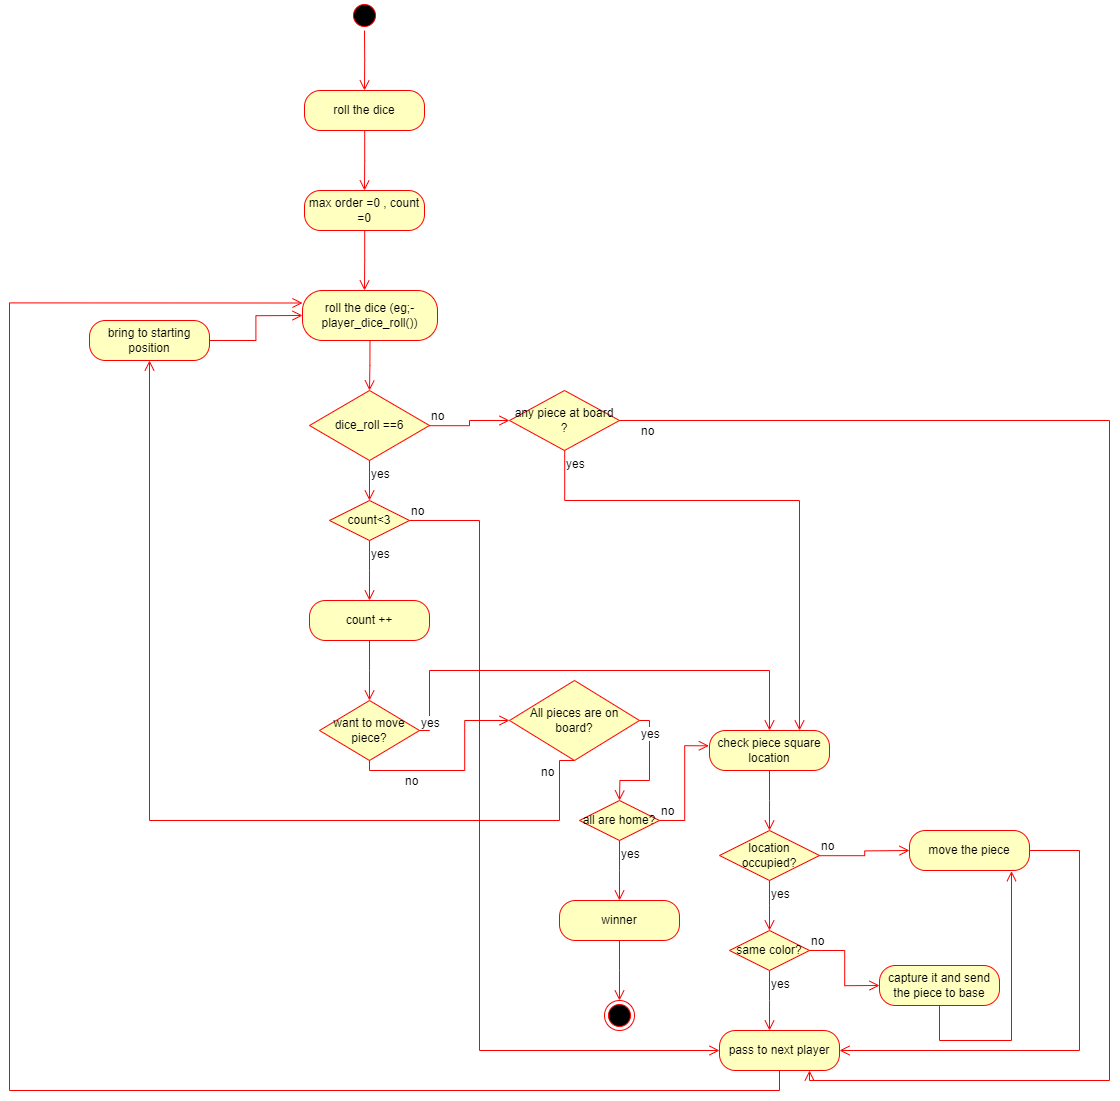
\includegraphics[width=492.55pt,height=484.2pt]{latexImage_9f3ed95fcb933e12bd292c7beefd1cd7.png}}
\put(57.024,-80.85999){\fontsize{20.04}{1}\usefont{T1}{cmr}{m}{n}\selectfont\color{color_46504}1.Classical Ludo Flow Chart }
\put(57.024,-107.26){\fontsize{20.04}{1}\usefont{T1}{cmr}{m}{n}\selectfont\color{color_46504} }
\put(57.024,-128.98){\fontsize{11.04}{1}\usefont{T1}{cmr}{m}{n}\selectfont\color{color_29791} }
\put(57.024,-151.54){\fontsize{11.04}{1}\usefont{T1}{cmr}{m}{n}\selectfont\color{color_29791} }
\put(57.024,-173.98){\fontsize{11.04}{1}\usefont{T1}{cmr}{m}{n}\selectfont\color{color_29791} }
\put(57.024,-196.54){\fontsize{11.04}{1}\usefont{T1}{cmr}{m}{n}\selectfont\color{color_29791} }
\put(57.024,-218.98){\fontsize{11.04}{1}\usefont{T1}{cmr}{m}{n}\selectfont\color{color_29791} }
\put(57.024,-241.57){\fontsize{11.04}{1}\usefont{T1}{cmr}{m}{n}\selectfont\color{color_29791} }
\put(57.024,-264.01){\fontsize{11.04}{1}\usefont{T1}{cmr}{m}{n}\selectfont\color{color_29791} }
\put(57.024,-286.45){\fontsize{11.04}{1}\usefont{T1}{cmr}{m}{n}\selectfont\color{color_29791} }
\put(57.024,-309.01){\fontsize{11.04}{1}\usefont{T1}{cmr}{m}{n}\selectfont\color{color_29791} }
\put(57.024,-331.45){\fontsize{11.04}{1}\usefont{T1}{cmr}{m}{n}\selectfont\color{color_29791} }
\put(57.024,-354.01){\fontsize{11.04}{1}\usefont{T1}{cmr}{m}{n}\selectfont\color{color_29791} }
\put(57.024,-376.45){\fontsize{11.04}{1}\usefont{T1}{cmr}{m}{n}\selectfont\color{color_29791} }
\put(57.024,-399.01){\fontsize{11.04}{1}\usefont{T1}{cmr}{m}{n}\selectfont\color{color_29791} }
\put(57.024,-421.47){\fontsize{11.04}{1}\usefont{T1}{cmr}{m}{n}\selectfont\color{color_29791} }
\put(57.024,-443.91){\fontsize{11.04}{1}\usefont{T1}{cmr}{m}{n}\selectfont\color{color_29791} }
\put(57.024,-466.47){\fontsize{11.04}{1}\usefont{T1}{cmr}{m}{n}\selectfont\color{color_29791} }
\put(57.024,-488.91){\fontsize{11.04}{1}\usefont{T1}{cmr}{m}{n}\selectfont\color{color_29791} }
\put(57.024,-511.47){\fontsize{11.04}{1}\usefont{T1}{cmr}{m}{n}\selectfont\color{color_29791} }
\put(57.024,-533.91){\fontsize{11.04}{1}\usefont{T1}{cmr}{m}{n}\selectfont\color{color_29791} }
\put(57.024,-556.35){\fontsize{11.04}{1}\usefont{T1}{cmr}{m}{n}\selectfont\color{color_29791} }
\put(57.024,-578.94){\fontsize{11.04}{1}\usefont{T1}{cmr}{m}{n}\selectfont\color{color_29791} }
\put(57.024,-601.38){\fontsize{11.04}{1}\usefont{T1}{cmr}{m}{n}\selectfont\color{color_29791} }
\put(57.024,-623.94){\fontsize{11.04}{1}\usefont{T1}{cmr}{m}{n}\selectfont\color{color_29791}This flow chart, as I see, captures main functions that needed to be in the classical ludo game.  }
\put(57.024,-646.38){\fontsize{11.04}{1}\usefont{T1}{cmr}{m}{n}\selectfont\color{color_29791} }
\put(57.024,-668.94){\fontsize{11.04}{1}\usefont{T1}{cmr}{m}{n}\selectfont\color{color_29791} }
\put(57.024,-691.376){\fontsize{11.04}{1}\usefont{T1}{cmr}{m}{n}\selectfont\color{color_29791}  }
\end{picture}
\begin{tikzpicture}[overlay]
\path(0pt,0pt);
\filldraw[color_283006][even odd rule]
(57pt, -607.35pt) -- (549.55pt, -607.35pt)
 -- (549.55pt, -607.35pt)
 -- (549.55pt, -586.35pt)
 -- (549.55pt, -586.35pt)
 -- (57pt, -586.35pt) -- cycle
;
\begin{scope}
\clip
(57.024pt, -607.38pt) -- (549.574pt, -607.38pt)
 -- (549.574pt, -607.38pt)
 -- (549.574pt, -586.5pt)
 -- (549.574pt, -586.5pt)
 -- (57.024pt, -586.5pt) -- cycle
;
\begin{scope}
\clip
(57.024pt, -607.38pt) -- (549.574pt, -607.38pt)
 -- (549.574pt, -607.38pt)
 -- (549.574pt, -586.5pt)
 -- (549.574pt, -586.5pt)
 -- (57.024pt, -586.5pt) -- cycle
;
\end{scope}
\end{scope}
\end{tikzpicture}
\begin{picture}(-5,0)(2.5,0)
\put(238.01,-595.02){\fontsize{9}{1}\usefont{T1}{cmr}{m}{it}\selectfont\color{color_44550}Figure 1 . classical ludo flow chart }
\end{picture}
\begin{tikzpicture}[overlay]
\path(0pt,0pt);
\filldraw[color_29791][even odd rule]
(9pt, -14.47998pt) -- (9.48pt, -14.47998pt)
 -- (9.48pt, -14.47998pt)
 -- (9.48pt, -14pt)
 -- (9.48pt, -14pt)
 -- (9pt, -14pt) -- cycle
;
\filldraw[color_29791][even odd rule]
(9pt, -14.47998pt) -- (9.48pt, -14.47998pt)
 -- (9.48pt, -14.47998pt)
 -- (9.48pt, -14pt)
 -- (9.48pt, -14pt)
 -- (9pt, -14pt) -- cycle
;
\filldraw[color_29791][even odd rule]
(9.48pt, -14.47998pt) -- (572.64pt, -14.47998pt)
 -- (572.64pt, -14.47998pt)
 -- (572.64pt, -14pt)
 -- (572.64pt, -14pt)
 -- (9.48pt, -14pt) -- cycle
;
\filldraw[color_29791][even odd rule]
(572.64pt, -14.47998pt) -- (573.12pt, -14.47998pt)
 -- (573.12pt, -14.47998pt)
 -- (573.12pt, -14pt)
 -- (573.12pt, -14pt)
 -- (572.64pt, -14pt) -- cycle
;
\filldraw[color_29791][even odd rule]
(572.64pt, -14.47998pt) -- (573.12pt, -14.47998pt)
 -- (573.12pt, -14.47998pt)
 -- (573.12pt, -14pt)
 -- (573.12pt, -14pt)
 -- (572.64pt, -14pt) -- cycle
;
\filldraw[color_29791][even odd rule]
(9pt, -757.64pt) -- (9.48pt, -757.64pt)
 -- (9.48pt, -757.64pt)
 -- (9.48pt, -14.48004pt)
 -- (9.48pt, -14.48004pt)
 -- (9pt, -14.48004pt) -- cycle
;
\filldraw[color_29791][even odd rule]
(572.64pt, -757.64pt) -- (573.12pt, -757.64pt)
 -- (573.12pt, -757.64pt)
 -- (573.12pt, -14.48004pt)
 -- (573.12pt, -14.48004pt)
 -- (572.64pt, -14.48004pt) -- cycle
;
\filldraw[color_29791][even odd rule]
(9pt, -758.12pt) -- (9.48pt, -758.12pt)
 -- (9.48pt, -758.12pt)
 -- (9.48pt, -757.64pt)
 -- (9.48pt, -757.64pt)
 -- (9pt, -757.64pt) -- cycle
;
\filldraw[color_29791][even odd rule]
(9pt, -758.12pt) -- (9.48pt, -758.12pt)
 -- (9.48pt, -758.12pt)
 -- (9.48pt, -757.64pt)
 -- (9.48pt, -757.64pt)
 -- (9pt, -757.64pt) -- cycle
;
\filldraw[color_29791][even odd rule]
(9.48pt, -758.12pt) -- (572.64pt, -758.12pt)
 -- (572.64pt, -758.12pt)
 -- (572.64pt, -757.64pt)
 -- (572.64pt, -757.64pt)
 -- (9.48pt, -757.64pt) -- cycle
;
\filldraw[color_29791][even odd rule]
(572.64pt, -758.12pt) -- (573.12pt, -758.12pt)
 -- (573.12pt, -758.12pt)
 -- (573.12pt, -757.64pt)
 -- (573.12pt, -757.64pt)
 -- (572.64pt, -757.64pt) -- cycle
;
\end{tikzpicture}
\newpage
\begin{tikzpicture}[overlay]
\path(0pt,0pt);
\filldraw[color_29791][even odd rule]
(572.64pt, -758.12pt) -- (573.12pt, -758.12pt)
 -- (573.12pt, -758.12pt)
 -- (573.12pt, -757.64pt)
 -- (573.12pt, -757.64pt)
 -- (572.64pt, -757.64pt) -- cycle
;
\begin{scope}
\clip
(10.05pt, -401.59pt) -- (573.75pt, -401.59pt)
 -- (573.75pt, -401.59pt)
 -- (573.75pt, -144.79pt)
 -- (573.75pt, -144.79pt)
 -- (10.05pt, -144.79pt) -- cycle
;
\end{scope}
\end{tikzpicture}
\begin{picture}(-5,0)(2.5,0)
\put(10.05,-401.5901){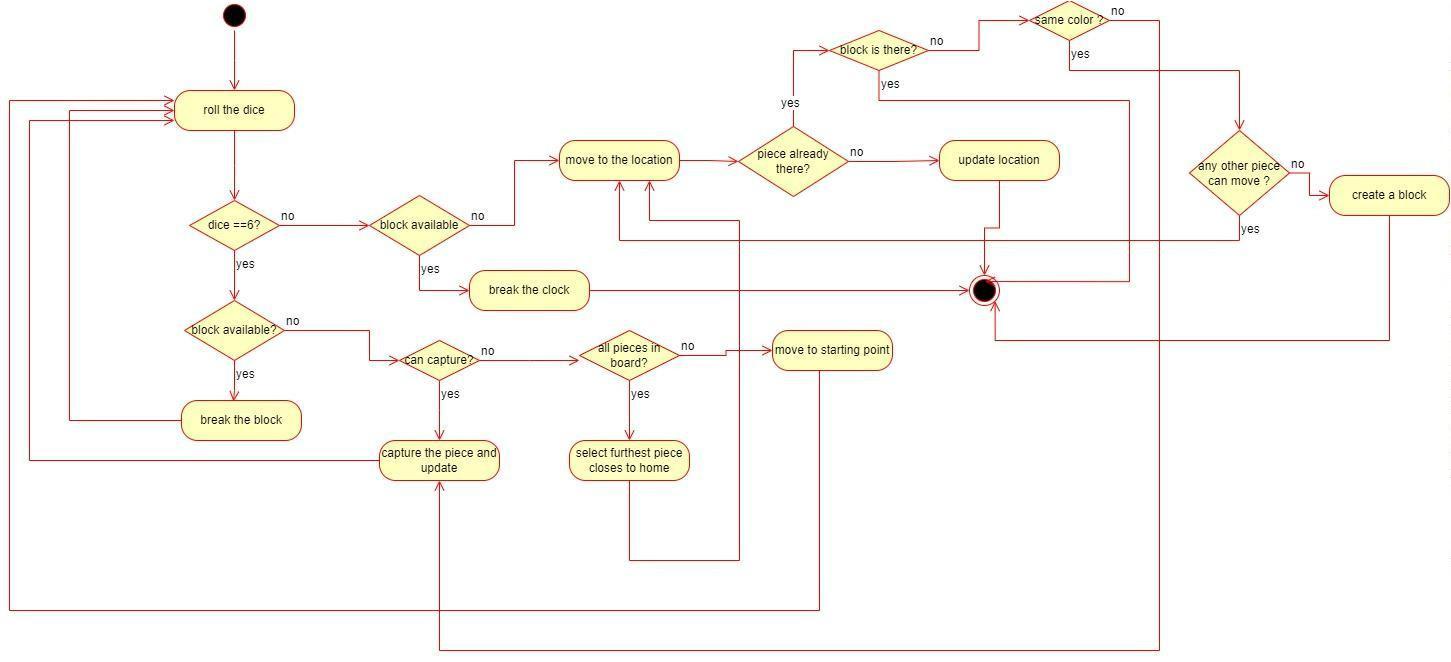
\includegraphics[width=563.7pt,height=256.8pt]{latexImage_89585a38dedc37e5655fcf506641c15f.png}}
\put(57.024,-80.85999){\fontsize{20.04}{1}\usefont{T1}{cmr}{m}{n}\selectfont\color{color_46504}2.Player behaviors flow charts }
\put(57.024,-125.26){\fontsize{20.04}{1}\usefont{T1}{cmr}{m}{n}\selectfont\color{color_46504} 2.1 Red Player }
\put(57.024,-146.98){\fontsize{11.04}{1}\usefont{T1}{cmr}{m}{n}\selectfont\color{color_29791} }
\put(57.024,-169.54){\fontsize{11.04}{1}\usefont{T1}{cmr}{m}{n}\selectfont\color{color_29791} }
\put(57.024,-191.98){\fontsize{11.04}{1}\usefont{T1}{cmr}{m}{n}\selectfont\color{color_29791} }
\put(57.024,-214.54){\fontsize{11.04}{1}\usefont{T1}{cmr}{m}{n}\selectfont\color{color_29791} }
\put(57.024,-237.01){\fontsize{11.04}{1}\usefont{T1}{cmr}{m}{n}\selectfont\color{color_29791} }
\put(57.024,-259.57){\fontsize{11.04}{1}\usefont{T1}{cmr}{m}{n}\selectfont\color{color_29791} }
\put(57.024,-282.01){\fontsize{11.04}{1}\usefont{T1}{cmr}{m}{n}\selectfont\color{color_29791} }
\put(57.024,-304.45){\fontsize{11.04}{1}\usefont{T1}{cmr}{m}{n}\selectfont\color{color_29791} }
\put(291.05,-327.01){\fontsize{11.04}{1}\usefont{T1}{cmr}{m}{n}\selectfont\color{color_29791} }
\put(57.024,-349.45){\fontsize{11.04}{1}\usefont{T1}{cmr}{m}{n}\selectfont\color{color_29791} }
\put(57.024,-372.01){\fontsize{11.04}{1}\usefont{T1}{cmr}{m}{n}\selectfont\color{color_29791} }
\put(57.024,-394.45){\fontsize{11.04}{1}\usefont{T1}{cmr}{m}{n}\selectfont\color{color_29791} }
\put(57.024,-417.03){\fontsize{11.04}{1}\usefont{T1}{cmr}{m}{n}\selectfont\color{color_29791} }
\put(57.024,-439.47){\fontsize{11.04}{1}\usefont{T1}{cmr}{m}{n}\selectfont\color{color_29791} }
\put(57.024,-461.91){\fontsize{11.04}{1}\usefont{T1}{cmr}{m}{n}\selectfont\color{color_29791}This flow chart captures the aggressive playing nature of the red player. The red player’s strategy will }
\put(57.024,-476.43){\fontsize{11.04}{1}\usefont{T1}{cmr}{m}{n}\selectfont\color{color_29791}be to win the game by playing aggressively by capturing when has a chance and creating a block }
\put(57.024,-490.95){\fontsize{11.04}{1}\usefont{T1}{cmr}{m}{n}\selectfont\color{color_29791}when there are no possible moves to make. }
\put(57.024,-513.39){\fontsize{11.04}{1}\usefont{T1}{cmr}{m}{n}\selectfont\color{color_29791} }
\put(57.024,-535.95){\fontsize{11.04}{1}\usefont{T1}{cmr}{m}{n}\selectfont\color{color_29791} }
\put(57.024,-558.39){\fontsize{11.04}{1}\usefont{T1}{cmr}{m}{n}\selectfont\color{color_29791} }
\put(57.024,-580.98){\fontsize{11.04}{1}\usefont{T1}{cmr}{m}{n}\selectfont\color{color_29791} }
\put(57.024,-603.42){\fontsize{11.04}{1}\usefont{T1}{cmr}{m}{n}\selectfont\color{color_29791} }
\put(57.024,-625.86){\fontsize{11.04}{1}\usefont{T1}{cmr}{m}{n}\selectfont\color{color_29791} }
\put(57.024,-648.42){\fontsize{11.04}{1}\usefont{T1}{cmr}{m}{n}\selectfont\color{color_29791} }
\put(57.024,-670.86){\fontsize{11.04}{1}\usefont{T1}{cmr}{m}{n}\selectfont\color{color_29791} }
\put(57.024,-693.416){\fontsize{11.04}{1}\usefont{T1}{cmr}{m}{n}\selectfont\color{color_29791} }
\end{picture}
\begin{tikzpicture}[overlay]
\path(0pt,0pt);
\filldraw[color_283006][even odd rule]
(-4.2pt, -443.3pt) -- (595.05pt, -443.3pt)
 -- (595.05pt, -443.3pt)
 -- (595.05pt, -422.3pt)
 -- (595.05pt, -422.3pt)
 -- (-4.2pt, -422.3pt) -- cycle
;
\begin{scope}
\clip
(-4.2pt, -443.31pt) -- (595.08pt, -443.31pt)
 -- (595.08pt, -443.31pt)
 -- (595.08pt, -422.43pt)
 -- (595.08pt, -422.43pt)
 -- (-4.2pt, -422.43pt) -- cycle
;
\begin{scope}
\clip
(-4.2pt, -443.31pt) -- (595.08pt, -443.31pt)
 -- (595.08pt, -443.31pt)
 -- (595.08pt, -422.43pt)
 -- (595.08pt, -422.43pt)
 -- (-4.2pt, -422.43pt) -- cycle
;
\end{scope}
\end{scope}
\end{tikzpicture}
\begin{picture}(-5,0)(2.5,0)
\put(237.29,-430.95){\fontsize{9}{1}\usefont{T1}{cmr}{m}{it}\selectfont\color{color_44550}Figure 2 (red player flow chart) }
\end{picture}
\begin{tikzpicture}[overlay]
\path(0pt,0pt);
\filldraw[color_29791][even odd rule]
(9pt, -14.47998pt) -- (9.48pt, -14.47998pt)
 -- (9.48pt, -14.47998pt)
 -- (9.48pt, -14pt)
 -- (9.48pt, -14pt)
 -- (9pt, -14pt) -- cycle
;
\filldraw[color_29791][even odd rule]
(9pt, -14.47998pt) -- (9.48pt, -14.47998pt)
 -- (9.48pt, -14.47998pt)
 -- (9.48pt, -14pt)
 -- (9.48pt, -14pt)
 -- (9pt, -14pt) -- cycle
;
\filldraw[color_29791][even odd rule]
(9.48pt, -14.47998pt) -- (572.64pt, -14.47998pt)
 -- (572.64pt, -14.47998pt)
 -- (572.64pt, -14pt)
 -- (572.64pt, -14pt)
 -- (9.48pt, -14pt) -- cycle
;
\filldraw[color_29791][even odd rule]
(572.64pt, -14.47998pt) -- (573.12pt, -14.47998pt)
 -- (573.12pt, -14.47998pt)
 -- (573.12pt, -14pt)
 -- (573.12pt, -14pt)
 -- (572.64pt, -14pt) -- cycle
;
\filldraw[color_29791][even odd rule]
(572.64pt, -14.47998pt) -- (573.12pt, -14.47998pt)
 -- (573.12pt, -14.47998pt)
 -- (573.12pt, -14pt)
 -- (573.12pt, -14pt)
 -- (572.64pt, -14pt) -- cycle
;
\filldraw[color_29791][even odd rule]
(9pt, -757.64pt) -- (9.48pt, -757.64pt)
 -- (9.48pt, -757.64pt)
 -- (9.48pt, -14.48004pt)
 -- (9.48pt, -14.48004pt)
 -- (9pt, -14.48004pt) -- cycle
;
\filldraw[color_29791][even odd rule]
(572.64pt, -757.64pt) -- (573.12pt, -757.64pt)
 -- (573.12pt, -757.64pt)
 -- (573.12pt, -14.48004pt)
 -- (573.12pt, -14.48004pt)
 -- (572.64pt, -14.48004pt) -- cycle
;
\filldraw[color_29791][even odd rule]
(9pt, -758.12pt) -- (9.48pt, -758.12pt)
 -- (9.48pt, -758.12pt)
 -- (9.48pt, -757.64pt)
 -- (9.48pt, -757.64pt)
 -- (9pt, -757.64pt) -- cycle
;
\filldraw[color_29791][even odd rule]
(9pt, -758.12pt) -- (9.48pt, -758.12pt)
 -- (9.48pt, -758.12pt)
 -- (9.48pt, -757.64pt)
 -- (9.48pt, -757.64pt)
 -- (9pt, -757.64pt) -- cycle
;
\filldraw[color_29791][even odd rule]
(9.48pt, -758.12pt) -- (572.64pt, -758.12pt)
 -- (572.64pt, -758.12pt)
 -- (572.64pt, -757.64pt)
 -- (572.64pt, -757.64pt)
 -- (9.48pt, -757.64pt) -- cycle
;
\filldraw[color_29791][even odd rule]
(572.64pt, -758.12pt) -- (573.12pt, -758.12pt)
 -- (573.12pt, -758.12pt)
 -- (573.12pt, -757.64pt)
 -- (573.12pt, -757.64pt)
 -- (572.64pt, -757.64pt) -- cycle
;
\end{tikzpicture}
\newpage
\begin{tikzpicture}[overlay]
\path(0pt,0pt);
\filldraw[color_29791][even odd rule]
(572.64pt, -758.12pt) -- (573.12pt, -758.12pt)
 -- (573.12pt, -758.12pt)
 -- (573.12pt, -757.64pt)
 -- (573.12pt, -757.64pt)
 -- (572.64pt, -757.64pt) -- cycle
;
\begin{scope}
\clip
(27pt, -562.5pt) -- (554.99pt, -562.5pt)
 -- (554.99pt, -562.5pt)
 -- (554.99pt, -92.5pt)
 -- (554.99pt, -92.5pt)
 -- (27pt, -92.5pt) -- cycle
;
\end{scope}
\end{tikzpicture}
\begin{picture}(-5,0)(2.5,0)
\put(27,-562.5){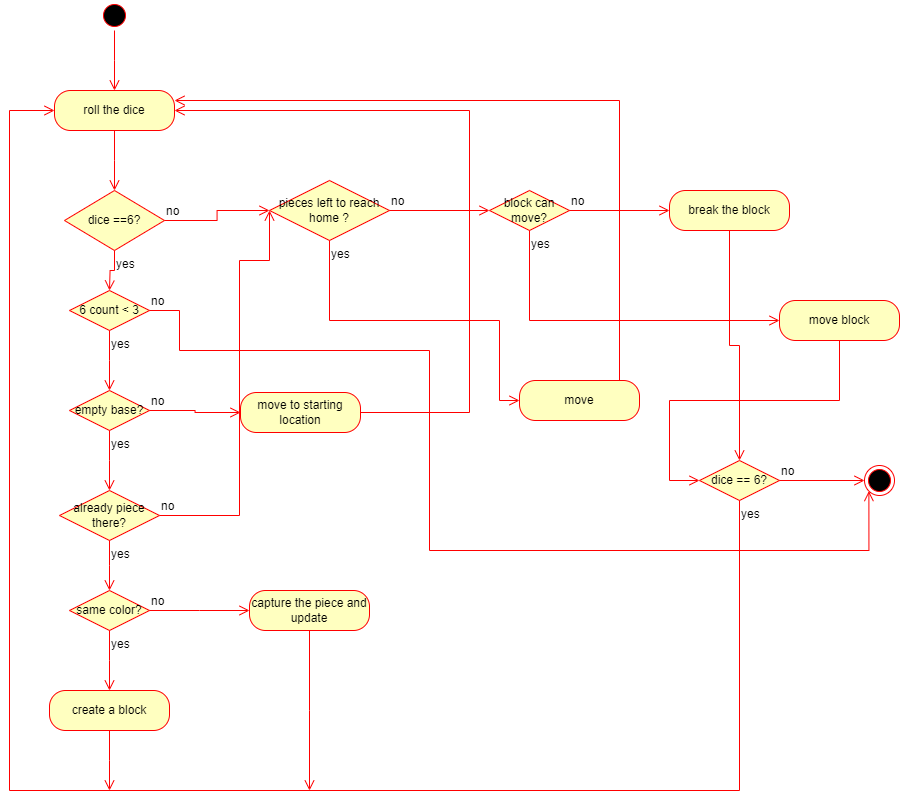
\includegraphics[width=527.99pt,height=470pt]{latexImage_e856a0fcde9ae77498e56918846c0b2c.png}}
\put(57.024,-80.85999){\fontsize{20.04}{1}\usefont{T1}{cmr}{m}{n}\selectfont\color{color_46504}2.2 Yellow Player }
\put(57.024,-102.7){\fontsize{11.04}{1}\usefont{T1}{cmr}{m}{n}\selectfont\color{color_29791} }
\put(57.024,-125.14){\fontsize{11.04}{1}\usefont{T1}{cmr}{m}{n}\selectfont\color{color_29791} }
\put(57.024,-147.7){\fontsize{11.04}{1}\usefont{T1}{cmr}{m}{n}\selectfont\color{color_29791} }
\put(57.024,-170.14){\fontsize{11.04}{1}\usefont{T1}{cmr}{m}{n}\selectfont\color{color_29791} }
\put(57.024,-192.7){\fontsize{11.04}{1}\usefont{T1}{cmr}{m}{n}\selectfont\color{color_29791} }
\put(57.024,-215.14){\fontsize{11.04}{1}\usefont{T1}{cmr}{m}{n}\selectfont\color{color_29791} }
\put(57.024,-237.61){\fontsize{11.04}{1}\usefont{T1}{cmr}{m}{n}\selectfont\color{color_29791} }
\put(57.024,-260.17){\fontsize{11.04}{1}\usefont{T1}{cmr}{m}{n}\selectfont\color{color_29791} }
\put(57.024,-282.61){\fontsize{11.04}{1}\usefont{T1}{cmr}{m}{n}\selectfont\color{color_29791} }
\put(57.024,-305.17){\fontsize{11.04}{1}\usefont{T1}{cmr}{m}{n}\selectfont\color{color_29791} }
\put(57.024,-327.61){\fontsize{11.04}{1}\usefont{T1}{cmr}{m}{n}\selectfont\color{color_29791} }
\put(57.024,-350.17){\fontsize{11.04}{1}\usefont{T1}{cmr}{m}{n}\selectfont\color{color_29791} }
\put(57.024,-372.61){\fontsize{11.04}{1}\usefont{T1}{cmr}{m}{n}\selectfont\color{color_29791} }
\put(57.024,-395.05){\fontsize{11.04}{1}\usefont{T1}{cmr}{m}{n}\selectfont\color{color_29791} }
\put(57.024,-417.63){\fontsize{11.04}{1}\usefont{T1}{cmr}{m}{n}\selectfont\color{color_29791} }
\put(57.024,-440.07){\fontsize{11.04}{1}\usefont{T1}{cmr}{m}{n}\selectfont\color{color_29791} }
\put(57.024,-462.63){\fontsize{11.04}{1}\usefont{T1}{cmr}{m}{n}\selectfont\color{color_29791} }
\put(57.024,-485.07){\fontsize{11.04}{1}\usefont{T1}{cmr}{m}{n}\selectfont\color{color_29791} }
\put(57.024,-507.51){\fontsize{11.04}{1}\usefont{T1}{cmr}{m}{n}\selectfont\color{color_29791} }
\put(57.024,-530.07){\fontsize{11.04}{1}\usefont{T1}{cmr}{m}{n}\selectfont\color{color_29791} }
\put(57.024,-552.51){\fontsize{11.04}{1}\usefont{T1}{cmr}{m}{n}\selectfont\color{color_29791} }
\put(57.024,-575.1){\fontsize{11.04}{1}\usefont{T1}{cmr}{m}{n}\selectfont\color{color_29791} }
\put(57.024,-597.54){\fontsize{11.04}{1}\usefont{T1}{cmr}{m}{n}\selectfont\color{color_29791} }
\put(57.024,-620.1){\fontsize{11.04}{1}\usefont{T1}{cmr}{m}{n}\selectfont\color{color_29791}This flow chart shows the yellow players’ playing behavior. Always trying to empty the base and }
\put(57.024,-634.5){\fontsize{11.04}{1}\usefont{T1}{cmr}{m}{n}\selectfont\color{color_29791}capturing processes and creating blocks are shown. }
\put(57.024,-657.06){\fontsize{11.04}{1}\usefont{T1}{cmr}{m}{n}\selectfont\color{color_29791} }
\put(57.024,-679.5){\fontsize{11.04}{1}\usefont{T1}{cmr}{m}{n}\selectfont\color{color_29791} }
\put(57.024,-702.056){\fontsize{11.04}{1}\usefont{T1}{cmr}{m}{n}\selectfont\color{color_29791} }
\end{picture}
\begin{tikzpicture}[overlay]
\path(0pt,0pt);
\filldraw[color_283006][even odd rule]
(27pt, -588pt) -- (555pt, -588pt)
 -- (555pt, -588pt)
 -- (555pt, -567pt)
 -- (555pt, -567pt)
 -- (27pt, -567pt) -- cycle
;
\begin{scope}
\clip
(27pt, -588.06pt) -- (555.1pt, -588.06pt)
 -- (555.1pt, -588.06pt)
 -- (555.1pt, -567.036pt)
 -- (555.1pt, -567.036pt)
 -- (27pt, -567.036pt) -- cycle
;
\begin{scope}
\clip
(27pt, -588.06pt) -- (555.1pt, -588.06pt)
 -- (555.1pt, -588.06pt)
 -- (555.1pt, -567.036pt)
 -- (555.1pt, -567.036pt)
 -- (27pt, -567.036pt) -- cycle
;
\end{scope}
\end{scope}
\end{tikzpicture}
\begin{picture}(-5,0)(2.5,0)
\put(226.85,-575.58){\fontsize{9}{1}\usefont{T1}{cmr}{m}{it}\selectfont\color{color_44550}Figure 3 (yellow player flow chart) }
\end{picture}
\begin{tikzpicture}[overlay]
\path(0pt,0pt);
\filldraw[color_29791][even odd rule]
(9pt, -14.47998pt) -- (9.48pt, -14.47998pt)
 -- (9.48pt, -14.47998pt)
 -- (9.48pt, -14pt)
 -- (9.48pt, -14pt)
 -- (9pt, -14pt) -- cycle
;
\filldraw[color_29791][even odd rule]
(9pt, -14.47998pt) -- (9.48pt, -14.47998pt)
 -- (9.48pt, -14.47998pt)
 -- (9.48pt, -14pt)
 -- (9.48pt, -14pt)
 -- (9pt, -14pt) -- cycle
;
\filldraw[color_29791][even odd rule]
(9.48pt, -14.47998pt) -- (572.64pt, -14.47998pt)
 -- (572.64pt, -14.47998pt)
 -- (572.64pt, -14pt)
 -- (572.64pt, -14pt)
 -- (9.48pt, -14pt) -- cycle
;
\filldraw[color_29791][even odd rule]
(572.64pt, -14.47998pt) -- (573.12pt, -14.47998pt)
 -- (573.12pt, -14.47998pt)
 -- (573.12pt, -14pt)
 -- (573.12pt, -14pt)
 -- (572.64pt, -14pt) -- cycle
;
\filldraw[color_29791][even odd rule]
(572.64pt, -14.47998pt) -- (573.12pt, -14.47998pt)
 -- (573.12pt, -14.47998pt)
 -- (573.12pt, -14pt)
 -- (573.12pt, -14pt)
 -- (572.64pt, -14pt) -- cycle
;
\filldraw[color_29791][even odd rule]
(9pt, -757.64pt) -- (9.48pt, -757.64pt)
 -- (9.48pt, -757.64pt)
 -- (9.48pt, -14.48004pt)
 -- (9.48pt, -14.48004pt)
 -- (9pt, -14.48004pt) -- cycle
;
\filldraw[color_29791][even odd rule]
(572.64pt, -757.64pt) -- (573.12pt, -757.64pt)
 -- (573.12pt, -757.64pt)
 -- (573.12pt, -14.48004pt)
 -- (573.12pt, -14.48004pt)
 -- (572.64pt, -14.48004pt) -- cycle
;
\filldraw[color_29791][even odd rule]
(9pt, -758.12pt) -- (9.48pt, -758.12pt)
 -- (9.48pt, -758.12pt)
 -- (9.48pt, -757.64pt)
 -- (9.48pt, -757.64pt)
 -- (9pt, -757.64pt) -- cycle
;
\filldraw[color_29791][even odd rule]
(9pt, -758.12pt) -- (9.48pt, -758.12pt)
 -- (9.48pt, -758.12pt)
 -- (9.48pt, -757.64pt)
 -- (9.48pt, -757.64pt)
 -- (9pt, -757.64pt) -- cycle
;
\filldraw[color_29791][even odd rule]
(9.48pt, -758.12pt) -- (572.64pt, -758.12pt)
 -- (572.64pt, -758.12pt)
 -- (572.64pt, -757.64pt)
 -- (572.64pt, -757.64pt)
 -- (9.48pt, -757.64pt) -- cycle
;
\filldraw[color_29791][even odd rule]
(572.64pt, -758.12pt) -- (573.12pt, -758.12pt)
 -- (573.12pt, -758.12pt)
 -- (573.12pt, -757.64pt)
 -- (573.12pt, -757.64pt)
 -- (572.64pt, -757.64pt) -- cycle
;
\end{tikzpicture}
\newpage
\begin{tikzpicture}[overlay]
\path(0pt,0pt);
\filldraw[color_29791][even odd rule]
(572.64pt, -758.12pt) -- (573.12pt, -758.12pt)
 -- (573.12pt, -758.12pt)
 -- (573.12pt, -757.64pt)
 -- (573.12pt, -757.64pt)
 -- (572.64pt, -757.64pt) -- cycle
;
\begin{scope}
\clip
(27.5pt, -645.49pt) -- (561.5pt, -645.49pt)
 -- (561.5pt, -645.49pt)
 -- (561.5pt, -147.49pt)
 -- (561.5pt, -147.49pt)
 -- (27.5pt, -147.49pt) -- cycle
;
\end{scope}
\end{tikzpicture}
\begin{picture}(-5,0)(2.5,0)
\put(27.5,-645.49){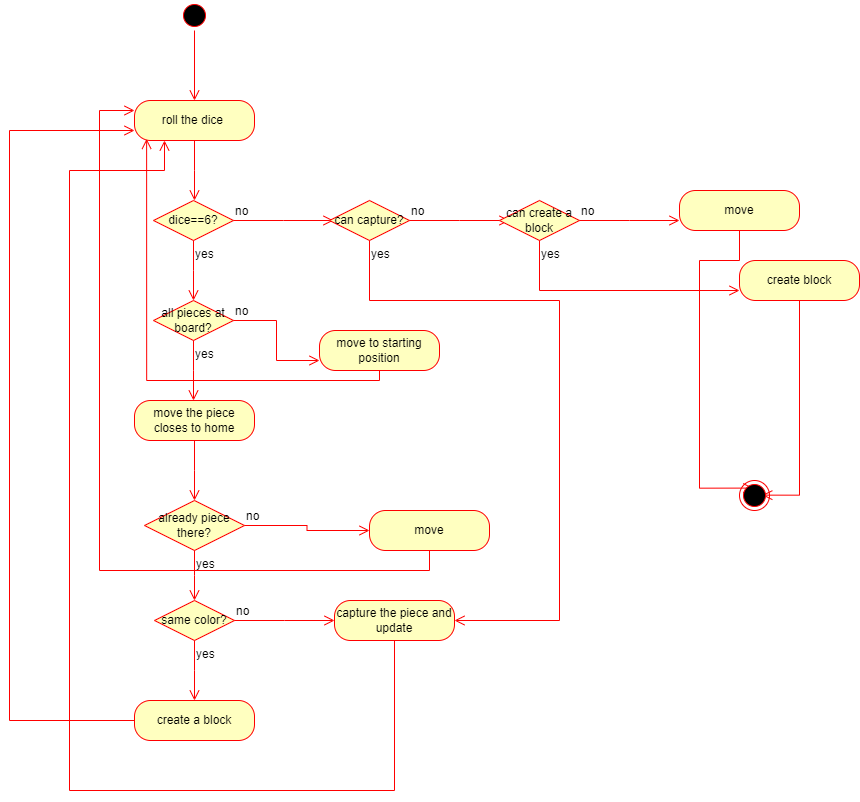
\includegraphics[width=534pt,height=498pt]{latexImage_59457ba052fb19dc8720af35da01f4a3.png}}
\put(57.024,-72.34003){\fontsize{11.04}{1}\usefont{T1}{cmr}{m}{n}\selectfont\color{color_29791} }
\put(57.024,-113.26){\fontsize{20.04}{1}\usefont{T1}{cmr}{m}{n}\selectfont\color{color_46504}2.3 Green Player  }
\put(57.024,-135.22){\fontsize{11.04}{1}\usefont{T1}{cmr}{m}{n}\selectfont\color{color_29791} }
\put(57.024,-157.66){\fontsize{11.04}{1}\usefont{T1}{cmr}{m}{n}\selectfont\color{color_29791} }
\put(57.024,-180.1){\fontsize{11.04}{1}\usefont{T1}{cmr}{m}{n}\selectfont\color{color_29791} }
\put(57.024,-202.66){\fontsize{11.04}{1}\usefont{T1}{cmr}{m}{n}\selectfont\color{color_29791} }
\put(57.024,-225.1){\fontsize{11.04}{1}\usefont{T1}{cmr}{m}{n}\selectfont\color{color_29791} }
\put(57.024,-247.69){\fontsize{11.04}{1}\usefont{T1}{cmr}{m}{n}\selectfont\color{color_29791} }
\put(57.024,-270.13){\fontsize{11.04}{1}\usefont{T1}{cmr}{m}{n}\selectfont\color{color_29791} }
\put(57.024,-292.69){\fontsize{11.04}{1}\usefont{T1}{cmr}{m}{n}\selectfont\color{color_29791} }
\put(57.024,-315.13){\fontsize{11.04}{1}\usefont{T1}{cmr}{m}{n}\selectfont\color{color_29791} }
\put(57.024,-337.57){\fontsize{11.04}{1}\usefont{T1}{cmr}{m}{n}\selectfont\color{color_29791} }
\put(57.024,-360.13){\fontsize{11.04}{1}\usefont{T1}{cmr}{m}{n}\selectfont\color{color_29791} }
\put(57.024,-382.57){\fontsize{11.04}{1}\usefont{T1}{cmr}{m}{n}\selectfont\color{color_29791} }
\put(57.024,-405.15){\fontsize{11.04}{1}\usefont{T1}{cmr}{m}{n}\selectfont\color{color_29791} }
\put(57.024,-427.59){\fontsize{11.04}{1}\usefont{T1}{cmr}{m}{n}\selectfont\color{color_29791} }
\put(57.024,-450.15){\fontsize{11.04}{1}\usefont{T1}{cmr}{m}{n}\selectfont\color{color_29791} }
\put(57.024,-472.59){\fontsize{11.04}{1}\usefont{T1}{cmr}{m}{n}\selectfont\color{color_29791} }
\put(57.024,-495.03){\fontsize{11.04}{1}\usefont{T1}{cmr}{m}{n}\selectfont\color{color_29791} }
\put(57.024,-517.59){\fontsize{11.04}{1}\usefont{T1}{cmr}{m}{n}\selectfont\color{color_29791} }
\put(57.024,-540.03){\fontsize{11.04}{1}\usefont{T1}{cmr}{m}{n}\selectfont\color{color_29791} }
\put(57.024,-562.59){\fontsize{11.04}{1}\usefont{T1}{cmr}{m}{n}\selectfont\color{color_29791} }
\put(57.024,-585.06){\fontsize{11.04}{1}\usefont{T1}{cmr}{m}{n}\selectfont\color{color_29791} }
\put(57.024,-607.62){\fontsize{11.04}{1}\usefont{T1}{cmr}{m}{n}\selectfont\color{color_29791} }
\put(57.024,-630.06){\fontsize{11.04}{1}\usefont{T1}{cmr}{m}{n}\selectfont\color{color_29791} }
\put(57.024,-652.5){\fontsize{11.04}{1}\usefont{T1}{cmr}{m}{n}\selectfont\color{color_29791} }
\put(57.024,-675.06){\fontsize{11.04}{1}\usefont{T1}{cmr}{m}{n}\selectfont\color{color_29791} }
\put(57.024,-697.496){\fontsize{11.04}{1}\usefont{T1}{cmr}{m}{n}\selectfont\color{color_29791}This shows the prioritizing moving piece to the home behavior and creating block behavior of green. }
\end{picture}
\begin{tikzpicture}[overlay]
\path(0pt,0pt);
\filldraw[color_283006][even odd rule]
(27.5pt, -671pt) -- (561.5pt, -671pt)
 -- (561.5pt, -671pt)
 -- (561.5pt, -650pt)
 -- (561.5pt, -650pt)
 -- (27.5pt, -650pt) -- cycle
;
\begin{scope}
\clip
(27.48pt, -671.1pt) -- (561.58pt, -671.1pt)
 -- (561.58pt, -671.1pt)
 -- (561.58pt, -650.1pt)
 -- (561.58pt, -650.1pt)
 -- (27.48pt, -650.1pt) -- cycle
;
\begin{scope}
\clip
(27.48pt, -671.1pt) -- (561.58pt, -671.1pt)
 -- (561.58pt, -671.1pt)
 -- (561.58pt, -650.1pt)
 -- (561.58pt, -650.1pt)
 -- (27.48pt, -650.1pt) -- cycle
;
\end{scope}
\end{scope}
\end{tikzpicture}
\begin{picture}(-5,0)(2.5,0)
\put(231.77,-658.62){\fontsize{9}{1}\usefont{T1}{cmr}{m}{it}\selectfont\color{color_44550}Figure 4 (green player flow chart) }
\end{picture}
\begin{tikzpicture}[overlay]
\path(0pt,0pt);
\filldraw[color_29791][even odd rule]
(9pt, -14.47998pt) -- (9.48pt, -14.47998pt)
 -- (9.48pt, -14.47998pt)
 -- (9.48pt, -14pt)
 -- (9.48pt, -14pt)
 -- (9pt, -14pt) -- cycle
;
\filldraw[color_29791][even odd rule]
(9pt, -14.47998pt) -- (9.48pt, -14.47998pt)
 -- (9.48pt, -14.47998pt)
 -- (9.48pt, -14pt)
 -- (9.48pt, -14pt)
 -- (9pt, -14pt) -- cycle
;
\filldraw[color_29791][even odd rule]
(9.48pt, -14.47998pt) -- (572.64pt, -14.47998pt)
 -- (572.64pt, -14.47998pt)
 -- (572.64pt, -14pt)
 -- (572.64pt, -14pt)
 -- (9.48pt, -14pt) -- cycle
;
\filldraw[color_29791][even odd rule]
(572.64pt, -14.47998pt) -- (573.12pt, -14.47998pt)
 -- (573.12pt, -14.47998pt)
 -- (573.12pt, -14pt)
 -- (573.12pt, -14pt)
 -- (572.64pt, -14pt) -- cycle
;
\filldraw[color_29791][even odd rule]
(572.64pt, -14.47998pt) -- (573.12pt, -14.47998pt)
 -- (573.12pt, -14.47998pt)
 -- (573.12pt, -14pt)
 -- (573.12pt, -14pt)
 -- (572.64pt, -14pt) -- cycle
;
\filldraw[color_29791][even odd rule]
(9pt, -757.64pt) -- (9.48pt, -757.64pt)
 -- (9.48pt, -757.64pt)
 -- (9.48pt, -14.48004pt)
 -- (9.48pt, -14.48004pt)
 -- (9pt, -14.48004pt) -- cycle
;
\filldraw[color_29791][even odd rule]
(572.64pt, -757.64pt) -- (573.12pt, -757.64pt)
 -- (573.12pt, -757.64pt)
 -- (573.12pt, -14.48004pt)
 -- (573.12pt, -14.48004pt)
 -- (572.64pt, -14.48004pt) -- cycle
;
\filldraw[color_29791][even odd rule]
(9pt, -758.12pt) -- (9.48pt, -758.12pt)
 -- (9.48pt, -758.12pt)
 -- (9.48pt, -757.64pt)
 -- (9.48pt, -757.64pt)
 -- (9pt, -757.64pt) -- cycle
;
\filldraw[color_29791][even odd rule]
(9pt, -758.12pt) -- (9.48pt, -758.12pt)
 -- (9.48pt, -758.12pt)
 -- (9.48pt, -757.64pt)
 -- (9.48pt, -757.64pt)
 -- (9pt, -757.64pt) -- cycle
;
\filldraw[color_29791][even odd rule]
(9.48pt, -758.12pt) -- (572.64pt, -758.12pt)
 -- (572.64pt, -758.12pt)
 -- (572.64pt, -757.64pt)
 -- (572.64pt, -757.64pt)
 -- (9.48pt, -757.64pt) -- cycle
;
\filldraw[color_29791][even odd rule]
(572.64pt, -758.12pt) -- (573.12pt, -758.12pt)
 -- (573.12pt, -758.12pt)
 -- (573.12pt, -757.64pt)
 -- (573.12pt, -757.64pt)
 -- (572.64pt, -757.64pt) -- cycle
;
\filldraw[color_29791][even odd rule]
(572.64pt, -758.12pt) -- (573.12pt, -758.12pt)
 -- (573.12pt, -758.12pt)
 -- (573.12pt, -757.64pt)
 -- (573.12pt, -757.64pt)
 -- (572.64pt, -757.64pt) -- cycle
;
\end{tikzpicture}
\newpage
\begin{tikzpicture}[overlay]\path(0pt,0pt);\end{tikzpicture}
\begin{picture}(-5,0)(2.5,0)
\put(57.024,-80.85999){\fontsize{20.04}{1}\usefont{T1}{cmr}{m}{n}\selectfont\color{color_46504}Thoughts on the Project's Initial Flowcharts and Their }
\put(57.024,-107.14){\fontsize{20.04}{1}\usefont{T1}{cmr}{m}{n}\selectfont\color{color_46504}Effect }
\put(57.024,-133.06){\fontsize{11.04}{1}\usefont{T1}{cmr}{m}{n}\selectfont\color{color_29791} }
\put(57.024,-147.58){\fontsize{11.04}{1}\usefont{T1}{cmr}{m}{n}\selectfont\color{color_29791}A fundamental, if somewhat simplistic, depiction of the project's procedures was given by the }
\put(57.024,-161.98){\fontsize{11.04}{1}\usefont{T1}{cmr}{m}{n}\selectfont\color{color_29791}flowcharts that were previously supplied (Figures 1 to 4). The development process benefited }
\put(57.024,-176.5){\fontsize{11.04}{1}\usefont{T1}{cmr}{m}{n}\selectfont\color{color_29791}greatly from these diagrams, even though they might not accurately depict the subtleties and }
\put(57.024,-191.02){\fontsize{11.04}{1}\usefont{T1}{cmr}{m}{n}\selectfont\color{color_29791}complexity of the finished product. }
\put(57.024,-205.54){\fontsize{11.04}{1}\usefont{T1}{cmr}{m}{n}\selectfont\color{color_29791} }
\put(57.024,-219.94){\fontsize{11.04}{1}\usefont{T1}{cmr}{m}{n}\selectfont\color{color_29791}Even though they were straightforward, these early flowcharts helped direct my design and coding }
\put(57.024,-234.46){\fontsize{11.04}{1}\usefont{T1}{cmr}{m}{n}\selectfont\color{color_29791}efforts in the right directions. They made it possible for me to see how the software is organized and }
\put(57.024,-249.01){\fontsize{11.04}{1}\usefont{T1}{cmr}{m}{n}\selectfont\color{color_29791}flows generally, which made it easier for me to pinpoint its main elements and possible problems. }
\put(57.024,-263.53){\fontsize{11.04}{1}\usefont{T1}{cmr}{m}{n}\selectfont\color{color_29791}Flowcharts offered a road map for the creation of more intricate and precise algorithms by }
\put(57.024,-277.93){\fontsize{11.04}{1}\usefont{T1}{cmr}{m}{n}\selectfont\color{color_29791}decomposing the problem into smaller, more manageable components. }
\put(57.024,-292.45){\fontsize{11.04}{1}\usefont{T1}{cmr}{m}{n}\selectfont\color{color_29791} }
\put(57.024,-315.01){\fontsize{11.04}{1}\usefont{T1}{cmr}{m}{n}\selectfont\color{color_29791}The flowcharts have some advantages despite their shortcomings in terms of precision and detail: }
\put(57.024,-337.45){\fontsize{11.04}{1}\usefont{T1}{cmr}{m}{n}\selectfont\color{color_29791} }
\put(57.024,-351.97){\fontsize{11.04}{1}\usefont{T1}{cmr}{m}{n}\selectfont\color{color_29791} Conceptual Clarity: They supported the establishment of a clear foundation for subsequent }
\put(57.024,-366.37){\fontsize{11.04}{1}\usefont{T1}{cmr}{m}{n}\selectfont\color{color_29791}development and ideation by elucidating the basic ideas and procedures that had to be covered in }
\put(57.024,-380.89){\fontsize{11.04}{1}\usefont{T1}{cmr}{m}{n}\selectfont\color{color_29791}the code. }
\put(57.024,-395.41){\fontsize{11.04}{1}\usefont{T1}{cmr}{m}{n}\selectfont\color{color_29791} }
\put(57.024,-409.95){\fontsize{11.04}{1}\usefont{T1}{cmr}{m}{n}\selectfont\color{color_29791}The identification of core processes was facilitated by the diagrams, which brought together }
\put(57.024,-424.35){\fontsize{11.04}{1}\usefont{T1}{cmr}{m}{n}\selectfont\color{color_29791}important activities including player movement, dice rolling mechanics, and piece status }
\put(57.024,-438.87){\fontsize{11.04}{1}\usefont{T1}{cmr}{m}{n}\selectfont\color{color_29791}management. These processes later became central to the development pipeline. }
\put(57.024,-453.39){\fontsize{11.04}{1}\usefont{T1}{cmr}{b}{n}\selectfont\color{color_29791} }
\put(57.024,-467.91){\fontsize{11.04}{1}\usefont{T1}{cmr}{b}{n}\selectfont\color{color_29791}Iterated Improvement: An iterative approach to problem-solving was encouraged by the }
\put(57.024,-482.43){\fontsize{11.04}{1}\usefont{T1}{cmr}{m}{n}\selectfont\color{color_29791}flowcharts' preliminary character. More accurate and effective solutions resulted from revisiting }
\put(57.024,-496.83){\fontsize{11.04}{1}\usefont{T1}{cmr}{m}{n}\selectfont\color{color_29791}and refining these designs as the project moved on. }
\put(57.024,-511.35){\fontsize{11.04}{1}\usefont{T1}{cmr}{m}{n}\selectfont\color{color_29791} }
\put(57.024,-525.87){\fontsize{11.04}{1}\usefont{T1}{cmr}{m}{n}\selectfont\color{color_29791} }
\put(57.024,-540.39){\fontsize{11.04}{1}\usefont{T1}{cmr}{m}{n}\selectfont\color{color_29791}In summary, even if the original flowcharts may not have included every aspect of the finished }
\put(57.024,-554.79){\fontsize{11.04}{1}\usefont{T1}{cmr}{m}{n}\selectfont\color{color_29791}product, they played a crucial role in setting the my approach of project's foundation. With their }
\put(57.024,-569.31){\fontsize{11.04}{1}\usefont{T1}{cmr}{m}{n}\selectfont\color{color_29791}guidance and attention, I was able to approach the problem methodically, try out several }
\put(57.024,-583.86){\fontsize{11.04}{1}\usefont{T1}{cmr}{m}{n}\selectfont\color{color_29791}alternatives, and create a reliable and useful application. The value of visual planning tools in the }
\put(57.024,-598.38){\fontsize{11.04}{1}\usefont{T1}{cmr}{m}{n}\selectfont\color{color_29791}software development process is shown by the insights these diagrams provided, which were }
\put(57.024,-612.78){\fontsize{11.04}{1}\usefont{T1}{cmr}{m}{n}\selectfont\color{color_29791}crucial in turning abstract concepts into usable code. }
\put(57.024,-635.34){\fontsize{11.04}{1}\usefont{T1}{cmr}{m}{n}\selectfont\color{color_29791} }
\put(57.024,-657.78){\fontsize{11.04}{1}\usefont{T1}{cmr}{m}{n}\selectfont\color{color_29791} }
\end{picture}
\begin{tikzpicture}[overlay]
\path(0pt,0pt);
\filldraw[color_29791][even odd rule]
(9pt, -14.47998pt) -- (9.48pt, -14.47998pt)
 -- (9.48pt, -14.47998pt)
 -- (9.48pt, -14pt)
 -- (9.48pt, -14pt)
 -- (9pt, -14pt) -- cycle
;
\filldraw[color_29791][even odd rule]
(9pt, -14.47998pt) -- (9.48pt, -14.47998pt)
 -- (9.48pt, -14.47998pt)
 -- (9.48pt, -14pt)
 -- (9.48pt, -14pt)
 -- (9pt, -14pt) -- cycle
;
\filldraw[color_29791][even odd rule]
(9.48pt, -14.47998pt) -- (572.64pt, -14.47998pt)
 -- (572.64pt, -14.47998pt)
 -- (572.64pt, -14pt)
 -- (572.64pt, -14pt)
 -- (9.48pt, -14pt) -- cycle
;
\filldraw[color_29791][even odd rule]
(572.64pt, -14.47998pt) -- (573.12pt, -14.47998pt)
 -- (573.12pt, -14.47998pt)
 -- (573.12pt, -14pt)
 -- (573.12pt, -14pt)
 -- (572.64pt, -14pt) -- cycle
;
\filldraw[color_29791][even odd rule]
(572.64pt, -14.47998pt) -- (573.12pt, -14.47998pt)
 -- (573.12pt, -14.47998pt)
 -- (573.12pt, -14pt)
 -- (573.12pt, -14pt)
 -- (572.64pt, -14pt) -- cycle
;
\filldraw[color_29791][even odd rule]
(9pt, -757.64pt) -- (9.48pt, -757.64pt)
 -- (9.48pt, -757.64pt)
 -- (9.48pt, -14.48004pt)
 -- (9.48pt, -14.48004pt)
 -- (9pt, -14.48004pt) -- cycle
;
\filldraw[color_29791][even odd rule]
(572.64pt, -757.64pt) -- (573.12pt, -757.64pt)
 -- (573.12pt, -757.64pt)
 -- (573.12pt, -14.48004pt)
 -- (573.12pt, -14.48004pt)
 -- (572.64pt, -14.48004pt) -- cycle
;
\filldraw[color_29791][even odd rule]
(9pt, -758.12pt) -- (9.48pt, -758.12pt)
 -- (9.48pt, -758.12pt)
 -- (9.48pt, -757.64pt)
 -- (9.48pt, -757.64pt)
 -- (9pt, -757.64pt) -- cycle
;
\filldraw[color_29791][even odd rule]
(9pt, -758.12pt) -- (9.48pt, -758.12pt)
 -- (9.48pt, -758.12pt)
 -- (9.48pt, -757.64pt)
 -- (9.48pt, -757.64pt)
 -- (9pt, -757.64pt) -- cycle
;
\filldraw[color_29791][even odd rule]
(9.48pt, -758.12pt) -- (572.64pt, -758.12pt)
 -- (572.64pt, -758.12pt)
 -- (572.64pt, -757.64pt)
 -- (572.64pt, -757.64pt)
 -- (9.48pt, -757.64pt) -- cycle
;
\filldraw[color_29791][even odd rule]
(572.64pt, -758.12pt) -- (573.12pt, -758.12pt)
 -- (573.12pt, -758.12pt)
 -- (573.12pt, -757.64pt)
 -- (573.12pt, -757.64pt)
 -- (572.64pt, -757.64pt) -- cycle
;
\filldraw[color_29791][even odd rule]
(572.64pt, -758.12pt) -- (573.12pt, -758.12pt)
 -- (573.12pt, -758.12pt)
 -- (573.12pt, -757.64pt)
 -- (573.12pt, -757.64pt)
 -- (572.64pt, -757.64pt) -- cycle
;
\end{tikzpicture}
\newpage
\begin{tikzpicture}[overlay]\path(0pt,0pt);\end{tikzpicture}
\begin{picture}(-5,0)(2.5,0)
\put(57.024,-80.85999){\fontsize{20.04}{1}\usefont{T1}{cmr}{m}{n}\selectfont\color{color_46504}Code Justification }
\put(57.024,-102.7){\fontsize{11.04}{1}\usefont{T1}{cmr}{m}{n}\selectfont\color{color_29791}1.Player Status Loop: }
\put(75.024,-125.14){\fontsize{9.96}{1}\usefont{T1}{cmr}{m}{n}\selectfont\color{color_29791}• The function begins by looping through all the players using a for loop (for(int i=0; }
\put(93.02,-139.66){\fontsize{11.04}{1}\usefont{T1}{cmr}{m}{n}\selectfont\color{color_29791}i<NUM\_PLAYERS; i++)). }
\put(75.024,-162.1){\fontsize{9.96}{1}\usefont{T1}{cmr}{m}{n}\selectfont\color{color_29791}• For each player, it prints out the number of pieces on the board and in the base using the }
\put(93.02,-176.62){\fontsize{11.04}{1}\usefont{T1}{cmr}{m}{n}\selectfont\color{color_29791}player's color, piecesInBoard, and piecesInBase attributes. }
\put(57.024,-199.18){\fontsize{11.04}{1}\usefont{T1}{cmr}{m}{n}\selectfont\color{color_29791}2.Piece Location Information: }
\put(75.024,-221.62){\fontsize{9.96}{1}\usefont{T1}{cmr}{m}{n}\selectfont\color{color_29791}• After displaying the general status of the player's pieces, it prints a header indicating that }
\put(93.02,-236.17){\fontsize{11.04}{1}\usefont{T1}{cmr}{m}{n}\selectfont\color{color_29791}the locations of the player's pieces will be listed. }
\put(75.024,-258.61){\fontsize{9.96}{1}\usefont{T1}{cmr}{m}{n}\selectfont\color{color_29791}• The function then loops through each of the player's pieces (for(int j=0; j<4; j++)), checking }
\put(93.02,-273.13){\fontsize{11.04}{1}\usefont{T1}{cmr}{m}{n}\selectfont\color{color_29791}the status of each piece and printing its location or position accordingly: }
\put(111.02,-295.57){\fontsize{9.96}{1}\usefont{T1}{cmr}{m}{n}\selectfont\color{color_29791}o Base: If the piece is in the base (status == BASE), it prints that the piece is in the }
\put(129.02,-310.09){\fontsize{11.04}{1}\usefont{T1}{cmr}{m}{n}\selectfont\color{color_29791}base. }
\put(111.02,-332.65){\fontsize{9.96}{1}\usefont{T1}{cmr}{m}{n}\selectfont\color{color_29791}o Home: If the piece has reached home (status == HOME), it prints that the piece is in }
\put(129.02,-347.05){\fontsize{11.04}{1}\usefont{T1}{cmr}{m}{n}\selectfont\color{color_29791}home. }
\put(111.02,-369.61){\fontsize{9.96}{1}\usefont{T1}{cmr}{m}{n}\selectfont\color{color_29791}o Home Straight: If the piece is in the home straight (status == HOME\_STRAIGHT), it }
\put(129.02,-384.13){\fontsize{11.04}{1}\usefont{T1}{cmr}{m}{n}\selectfont\color{color_29791}prints that the piece is in the home straight. }
\put(111.02,-406.59){\fontsize{9.96}{1}\usefont{T1}{cmr}{m}{n}\selectfont\color{color_29791}o Board: If the piece is on the board (status == BOARD), it prints the piece's location }
\put(129.02,-421.11){\fontsize{11.04}{1}\usefont{T1}{cmr}{m}{n}\selectfont\color{color_29791}on the board. }
\put(57.024,-443.55){\fontsize{11.04}{1}\usefont{T1}{cmr}{m}{n}\selectfont\color{color_29791} }
\put(57.024,-466.11){\fontsize{11.04}{1}\usefont{T1}{cmr}{b}{n}\selectfont\color{color_29791}3.findPlayerIndexByColor(Player players[], const char* color) }
\put(75.024,-488.55){\fontsize{9.96}{1}\usefont{T1}{cmr}{m}{n}\selectfont\color{color_29791}• Purpose: Finds the index of a player based on their color. }
\put(75.024,-510.99){\fontsize{9.96}{1}\usefont{T1}{cmr}{m}{n}\selectfont\color{color_29791}• Functionality: }
\put(111.02,-533.55){\fontsize{9.96}{1}\usefont{T1}{cmr}{m}{n}\selectfont\color{color_29791}o Iterates through the players[] array. }
\put(111.02,-555.99){\fontsize{9.96}{1}\usefont{T1}{cmr}{m}{n}\selectfont\color{color_29791}o Compares each player's color with the provided color string using strcmp(). }
\put(111.02,-578.58){\fontsize{9.96}{1}\usefont{T1}{cmr}{m}{n}\selectfont\color{color_29791}o If a match is found, returns the index of that player. }
\put(111.02,-601.02){\fontsize{9.96}{1}\usefont{T1}{cmr}{m}{n}\selectfont\color{color_29791}o If no match is found, returns -1 to indicate the color was not found. }
\put(57.024,-623.58){\fontsize{11.04}{1}\usefont{T1}{cmr}{b}{n}\selectfont\color{color_29791}4. moveTostartingpoint(Player *player, int pieceIndex) (this is an underworking function) }
\put(75.024,-646.02){\fontsize{9.96}{1}\usefont{T1}{cmr}{m}{n}\selectfont\color{color_29791}• Purpose: Moves a player's piece from the base to the board's starting position. }
\put(75.024,-668.46){\fontsize{9.96}{1}\usefont{T1}{cmr}{m}{n}\selectfont\color{color_29791}• Functionality: }
\put(111.02,-691.016){\fontsize{9.96}{1}\usefont{T1}{cmr}{m}{n}\selectfont\color{color_29791}o Sets the direction of the piece using the toss() function (determines whether it will }
\put(129.02,-705.536){\fontsize{11.04}{1}\usefont{T1}{cmr}{m}{n}\selectfont\color{color_29791}move clockwise or counterclockwise). }
\end{picture}
\begin{tikzpicture}[overlay]
\path(0pt,0pt);
\filldraw[color_29791][even odd rule]
(9pt, -14.47998pt) -- (9.48pt, -14.47998pt)
 -- (9.48pt, -14.47998pt)
 -- (9.48pt, -14pt)
 -- (9.48pt, -14pt)
 -- (9pt, -14pt) -- cycle
;
\filldraw[color_29791][even odd rule]
(9pt, -14.47998pt) -- (9.48pt, -14.47998pt)
 -- (9.48pt, -14.47998pt)
 -- (9.48pt, -14pt)
 -- (9.48pt, -14pt)
 -- (9pt, -14pt) -- cycle
;
\filldraw[color_29791][even odd rule]
(9.48pt, -14.47998pt) -- (572.64pt, -14.47998pt)
 -- (572.64pt, -14.47998pt)
 -- (572.64pt, -14pt)
 -- (572.64pt, -14pt)
 -- (9.48pt, -14pt) -- cycle
;
\filldraw[color_29791][even odd rule]
(572.64pt, -14.47998pt) -- (573.12pt, -14.47998pt)
 -- (573.12pt, -14.47998pt)
 -- (573.12pt, -14pt)
 -- (573.12pt, -14pt)
 -- (572.64pt, -14pt) -- cycle
;
\filldraw[color_29791][even odd rule]
(572.64pt, -14.47998pt) -- (573.12pt, -14.47998pt)
 -- (573.12pt, -14.47998pt)
 -- (573.12pt, -14pt)
 -- (573.12pt, -14pt)
 -- (572.64pt, -14pt) -- cycle
;
\filldraw[color_29791][even odd rule]
(9pt, -757.64pt) -- (9.48pt, -757.64pt)
 -- (9.48pt, -757.64pt)
 -- (9.48pt, -14.48004pt)
 -- (9.48pt, -14.48004pt)
 -- (9pt, -14.48004pt) -- cycle
;
\filldraw[color_29791][even odd rule]
(572.64pt, -757.64pt) -- (573.12pt, -757.64pt)
 -- (573.12pt, -757.64pt)
 -- (573.12pt, -14.48004pt)
 -- (573.12pt, -14.48004pt)
 -- (572.64pt, -14.48004pt) -- cycle
;
\filldraw[color_29791][even odd rule]
(9pt, -758.12pt) -- (9.48pt, -758.12pt)
 -- (9.48pt, -758.12pt)
 -- (9.48pt, -757.64pt)
 -- (9.48pt, -757.64pt)
 -- (9pt, -757.64pt) -- cycle
;
\filldraw[color_29791][even odd rule]
(9pt, -758.12pt) -- (9.48pt, -758.12pt)
 -- (9.48pt, -758.12pt)
 -- (9.48pt, -757.64pt)
 -- (9.48pt, -757.64pt)
 -- (9pt, -757.64pt) -- cycle
;
\filldraw[color_29791][even odd rule]
(9.48pt, -758.12pt) -- (572.64pt, -758.12pt)
 -- (572.64pt, -758.12pt)
 -- (572.64pt, -757.64pt)
 -- (572.64pt, -757.64pt)
 -- (9.48pt, -757.64pt) -- cycle
;
\filldraw[color_29791][even odd rule]
(572.64pt, -758.12pt) -- (573.12pt, -758.12pt)
 -- (573.12pt, -758.12pt)
 -- (573.12pt, -757.64pt)
 -- (573.12pt, -757.64pt)
 -- (572.64pt, -757.64pt) -- cycle
;
\filldraw[color_29791][even odd rule]
(572.64pt, -758.12pt) -- (573.12pt, -758.12pt)
 -- (573.12pt, -758.12pt)
 -- (573.12pt, -757.64pt)
 -- (573.12pt, -757.64pt)
 -- (572.64pt, -757.64pt) -- cycle
;
\end{tikzpicture}
\newpage
\begin{tikzpicture}[overlay]\path(0pt,0pt);\end{tikzpicture}
\begin{picture}(-5,0)(2.5,0)
\put(111.02,-72.34003){\fontsize{9.96}{1}\usefont{T1}{cmr}{m}{n}\selectfont\color{color_29791}o Updates the piece’s status to BOARD, indicating it is now on the board. }
\put(111.02,-94.78003){\fontsize{9.96}{1}\usefont{T1}{cmr}{m}{n}\selectfont\color{color_29791}o Adjusts the player's count of pieces in the base and on the board. }
\put(111.02,-117.34){\fontsize{9.96}{1}\usefont{T1}{cmr}{m}{n}\selectfont\color{color_29791}o Sets the piece’s location based on the player's color (e.g., RX for Red, YX for Yellow). }
\put(111.02,-139.78){\fontsize{9.96}{1}\usefont{T1}{cmr}{m}{n}\selectfont\color{color_29791}o Increments the xpass attribute if the piece will move clockwise. }
\put(111.02,-162.34){\fontsize{9.96}{1}\usefont{T1}{cmr}{m}{n}\selectfont\color{color_29791}o Prints a message showing the piece’s new position and movement direction. }
\put(57.024,-184.78){\fontsize{11.04}{1}\usefont{T1}{cmr}{b}{n}\selectfont\color{color_29791}5. initializePlayer(Player* player, const char* color) }
\put(75.024,-207.34){\fontsize{9.96}{1}\usefont{T1}{cmr}{m}{n}\selectfont\color{color_29791}• Purpose: Initializes a player's attributes and their pieces at the start of the game. }
\put(75.024,-229.78){\fontsize{9.96}{1}\usefont{T1}{cmr}{m}{n}\selectfont\color{color_29791}• Functionality: }
\put(111.02,-252.25){\fontsize{9.96}{1}\usefont{T1}{cmr}{m}{n}\selectfont\color{color_29791}o Copies the player's color string to the player's color attribute. }
\put(111.02,-274.81){\fontsize{9.96}{1}\usefont{T1}{cmr}{m}{n}\selectfont\color{color_29791}o Sets the player's homeStart location based on their color. }
\put(111.02,-297.25){\fontsize{9.96}{1}\usefont{T1}{cmr}{m}{n}\selectfont\color{color_29791}o Initializes each piece: }
\put(147.02,-319.81){\fontsize{9.96}{1}\usefont{T1}{cmr}{m}{n}\selectfont\color{color_29791}▪ Assigns a unique ID (e.g., "R1" for Red piece 1). }
\put(147.02,-342.25){\fontsize{9.96}{1}\usefont{T1}{cmr}{m}{n}\selectfont\color{color_29791}▪ Sets the piece’s initial location to BASE\_LOCATION. }
\put(147.02,-364.69){\fontsize{9.96}{1}\usefont{T1}{cmr}{m}{n}\selectfont\color{color_29791}▪ Sets the piece’s status to BASE, indicating it starts in the base. }
\put(147.02,-387.25){\fontsize{9.96}{1}\usefont{T1}{cmr}{m}{n}\selectfont\color{color_29791}▪ Initializes attributes like captured, direction, xpass, and various status flags }
\put(165.02,-401.77){\fontsize{11.04}{1}\usefont{T1}{cmr}{m}{n}\selectfont\color{color_29791}(isBlocked, isEnergized, isSick, skipRounds). }
\put(111.02,-424.23){\fontsize{9.96}{1}\usefont{T1}{cmr}{m}{n}\selectfont\color{color_29791}o Initializes counters like piecesInHome, piecesInBoard, and piecesInBase. }
\put(57.024,-446.79){\fontsize{11.04}{1}\usefont{T1}{cmr}{b}{n}\selectfont\color{color_29791}6. move(Player* player, Player players[], int numPlayers) }
\put(75.024,-469.23){\fontsize{9.96}{1}\usefont{T1}{cmr}{m}{n}\selectfont\color{color_29791}• Purpose: Directs the player's move to the correct color-specific function. }
\put(75.024,-491.67){\fontsize{9.96}{1}\usefont{T1}{cmr}{m}{n}\selectfont\color{color_29791}• Functionality: }
\put(111.02,-514.23){\fontsize{9.96}{1}\usefont{T1}{cmr}{m}{n}\selectfont\color{color_29791}o Checks the player's color using strcmp(). }
\put(111.02,-536.67){\fontsize{9.96}{1}\usefont{T1}{cmr}{m}{n}\selectfont\color{color_29791}o Calls the corresponding move function (moveRed, moveYellow, moveGreen, or }
\put(129.02,-551.19){\fontsize{11.04}{1}\usefont{T1}{cmr}{m}{n}\selectfont\color{color_29791}moveBlue) based on the player's color. }
\put(57.024,-573.66){\fontsize{11.04}{1}\usefont{T1}{cmr}{b}{n}\selectfont\color{color_29791}7. rollDice() }
\put(75.024,-596.22){\fontsize{9.96}{1}\usefont{T1}{cmr}{m}{n}\selectfont\color{color_29791}• Purpose: Simulates rolling a six-sided dice. }
\put(75.024,-618.66){\fontsize{9.96}{1}\usefont{T1}{cmr}{m}{n}\selectfont\color{color_29791}• Functionality: }
\put(111.02,-641.22){\fontsize{9.96}{1}\usefont{T1}{cmr}{m}{n}\selectfont\color{color_29791}o Generates a random number between 1 and 6 using rand() \% 6 + 1. }
\put(111.02,-663.66){\fontsize{9.96}{1}\usefont{T1}{cmr}{m}{n}\selectfont\color{color_29791}o Returns the result of the dice roll. }
\put(57.024,-686.216){\fontsize{11.04}{1}\usefont{T1}{cmr}{m}{n}\selectfont\color{color_29791} }
\end{picture}
\begin{tikzpicture}[overlay]
\path(0pt,0pt);
\filldraw[color_29791][even odd rule]
(9pt, -14.47998pt) -- (9.48pt, -14.47998pt)
 -- (9.48pt, -14.47998pt)
 -- (9.48pt, -14pt)
 -- (9.48pt, -14pt)
 -- (9pt, -14pt) -- cycle
;
\filldraw[color_29791][even odd rule]
(9pt, -14.47998pt) -- (9.48pt, -14.47998pt)
 -- (9.48pt, -14.47998pt)
 -- (9.48pt, -14pt)
 -- (9.48pt, -14pt)
 -- (9pt, -14pt) -- cycle
;
\filldraw[color_29791][even odd rule]
(9.48pt, -14.47998pt) -- (572.64pt, -14.47998pt)
 -- (572.64pt, -14.47998pt)
 -- (572.64pt, -14pt)
 -- (572.64pt, -14pt)
 -- (9.48pt, -14pt) -- cycle
;
\filldraw[color_29791][even odd rule]
(572.64pt, -14.47998pt) -- (573.12pt, -14.47998pt)
 -- (573.12pt, -14.47998pt)
 -- (573.12pt, -14pt)
 -- (573.12pt, -14pt)
 -- (572.64pt, -14pt) -- cycle
;
\filldraw[color_29791][even odd rule]
(572.64pt, -14.47998pt) -- (573.12pt, -14.47998pt)
 -- (573.12pt, -14.47998pt)
 -- (573.12pt, -14pt)
 -- (573.12pt, -14pt)
 -- (572.64pt, -14pt) -- cycle
;
\filldraw[color_29791][even odd rule]
(9pt, -757.64pt) -- (9.48pt, -757.64pt)
 -- (9.48pt, -757.64pt)
 -- (9.48pt, -14.48004pt)
 -- (9.48pt, -14.48004pt)
 -- (9pt, -14.48004pt) -- cycle
;
\filldraw[color_29791][even odd rule]
(572.64pt, -757.64pt) -- (573.12pt, -757.64pt)
 -- (573.12pt, -757.64pt)
 -- (573.12pt, -14.48004pt)
 -- (573.12pt, -14.48004pt)
 -- (572.64pt, -14.48004pt) -- cycle
;
\filldraw[color_29791][even odd rule]
(9pt, -758.12pt) -- (9.48pt, -758.12pt)
 -- (9.48pt, -758.12pt)
 -- (9.48pt, -757.64pt)
 -- (9.48pt, -757.64pt)
 -- (9pt, -757.64pt) -- cycle
;
\filldraw[color_29791][even odd rule]
(9pt, -758.12pt) -- (9.48pt, -758.12pt)
 -- (9.48pt, -758.12pt)
 -- (9.48pt, -757.64pt)
 -- (9.48pt, -757.64pt)
 -- (9pt, -757.64pt) -- cycle
;
\filldraw[color_29791][even odd rule]
(9.48pt, -758.12pt) -- (572.64pt, -758.12pt)
 -- (572.64pt, -758.12pt)
 -- (572.64pt, -757.64pt)
 -- (572.64pt, -757.64pt)
 -- (9.48pt, -757.64pt) -- cycle
;
\filldraw[color_29791][even odd rule]
(572.64pt, -758.12pt) -- (573.12pt, -758.12pt)
 -- (573.12pt, -758.12pt)
 -- (573.12pt, -757.64pt)
 -- (573.12pt, -757.64pt)
 -- (572.64pt, -757.64pt) -- cycle
;
\filldraw[color_29791][even odd rule]
(572.64pt, -758.12pt) -- (573.12pt, -758.12pt)
 -- (573.12pt, -758.12pt)
 -- (573.12pt, -757.64pt)
 -- (573.12pt, -757.64pt)
 -- (572.64pt, -757.64pt) -- cycle
;
\end{tikzpicture}
\newpage
\begin{tikzpicture}[overlay]\path(0pt,0pt);\end{tikzpicture}
\begin{picture}(-5,0)(2.5,0)
\put(57.024,-72.34003){\fontsize{11.04}{1}\usefont{T1}{cmr}{m}{n}\selectfont\color{color_29791} }
\put(57.024,-86.85999){\fontsize{11.04}{1}\usefont{T1}{cmr}{b}{n}\selectfont\color{color_29791}8.capturePiece(Player* player, Player players[], int numPlayers) }
\put(75.024,-109.3){\fontsize{9.96}{1}\usefont{T1}{cmr}{m}{n}\selectfont\color{color_29791}• Purpose: Handles the capture of an opponent's piece when a player's piece lands on the }
\put(93.02,-123.82){\fontsize{11.04}{1}\usefont{T1}{cmr}{m}{n}\selectfont\color{color_29791}same square. }
\put(75.024,-146.26){\fontsize{9.96}{1}\usefont{T1}{cmr}{m}{n}\selectfont\color{color_29791}• Functionality: }
\put(111.02,-168.82){\fontsize{9.96}{1}\usefont{T1}{cmr}{m}{n}\selectfont\color{color_29791}o Loops through all opponents (other players). }
\put(111.02,-191.26){\fontsize{9.96}{1}\usefont{T1}{cmr}{m}{n}\selectfont\color{color_29791}o For each opponent, checks if any of their pieces are on the board (status == BOARD) }
\put(129.02,-205.78){\fontsize{11.04}{1}\usefont{T1}{cmr}{m}{n}\selectfont\color{color_29791}and if their location matches the current player’s piece location. }
\put(111.02,-228.22){\fontsize{9.96}{1}\usefont{T1}{cmr}{m}{n}\selectfont\color{color_29791}o If a match is found, it indicates a capture: }
\put(147.02,-250.81){\fontsize{9.96}{1}\usefont{T1}{cmr}{m}{n}\selectfont\color{color_29791}▪ The opponent's piece is returned to the base (status = BASE and location = }
\put(165.02,-265.33){\fontsize{11.04}{1}\usefont{T1}{cmr}{m}{n}\selectfont\color{color_29791}BASE\_LOCATION). }
\put(147.02,-287.77){\fontsize{9.96}{1}\usefont{T1}{cmr}{m}{n}\selectfont\color{color_29791}▪ Updates the opponent's counters (piecesInBoard decreases, piecesInBase }
\put(165.02,-302.29){\fontsize{11.04}{1}\usefont{T1}{cmr}{m}{n}\selectfont\color{color_29791}increases). }
\put(147.02,-324.73){\fontsize{9.96}{1}\usefont{T1}{cmr}{m}{n}\selectfont\color{color_29791}▪ Prints a message showing which piece was captured and its new location. }
\put(57.024,-347.29){\fontsize{11.04}{1}\usefont{T1}{cmr}{b}{n}\selectfont\color{color_29791}9. handleMysteryCell(Player *player, int pieceIndex, int mysteryEffect) }
\put(75.024,-369.73){\fontsize{9.96}{1}\usefont{T1}{cmr}{m}{n}\selectfont\color{color_29791}• Purpose: Applies the effect of landing on a mystery cell. }
\put(75.024,-392.17){\fontsize{9.96}{1}\usefont{T1}{cmr}{m}{n}\selectfont\color{color_29791}• Functionality: }
\put(111.02,-414.75){\fontsize{9.96}{1}\usefont{T1}{cmr}{m}{n}\selectfont\color{color_29791}o Based on the mysteryEffect value, the function applies one of several possible }
\put(129.02,-429.27){\fontsize{11.04}{1}\usefont{T1}{cmr}{m}{n}\selectfont\color{color_29791}effects: }
\put(147.02,-451.71){\fontsize{11.04}{1}\usefont{T1}{cmr}{m}{n}\selectfont\color{color_29791}1. Teleport: Moves the piece forward by 10 positions. }
\put(147.02,-474.15){\fontsize{11.04}{1}\usefont{T1}{cmr}{m}{n}\selectfont\color{color_29791}2. Energized: Doubles the piece's movement speed (isEnergized = 1). }
\put(147.02,-496.71){\fontsize{11.04}{1}\usefont{T1}{cmr}{m}{n}\selectfont\color{color_29791}3. Sick: Halves the piece's movement speed (isSick = 1). }
\put(147.02,-519.15){\fontsize{11.04}{1}\usefont{T1}{cmr}{m}{n}\selectfont\color{color_29791}4. Skip Rounds: Prevents the piece from moving for four rounds (skipRounds = }
\put(165.02,-533.67){\fontsize{11.04}{1}\usefont{T1}{cmr}{m}{n}\selectfont\color{color_29791}4). }
\put(147.02,-556.11){\fontsize{11.04}{1}\usefont{T1}{cmr}{m}{n}\selectfont\color{color_29791}5. Return to Base: Sends the piece back to the base (location = -1, status = }
\put(165.02,-570.63){\fontsize{11.04}{1}\usefont{T1}{cmr}{m}{n}\selectfont\color{color_29791}BASE, updates counters). }
\put(147.02,-593.22){\fontsize{11.04}{1}\usefont{T1}{cmr}{m}{n}\selectfont\color{color_29791}6. Change Direction: Reverses the piece's direction (direction *= -1). }
\put(111.02,-615.66){\fontsize{9.96}{1}\usefont{T1}{cmr}{m}{n}\selectfont\color{color_29791}o Prints a message describing the effect applied. }
\put(57.024,-638.22){\fontsize{11.04}{1}\usefont{T1}{cmr}{m}{n}\selectfont\color{color_29791} }
\put(57.024,-660.66){\fontsize{11.04}{1}\usefont{T1}{cmr}{m}{n}\selectfont\color{color_29791} }
\put(57.024,-683.096){\fontsize{11.04}{1}\usefont{T1}{cmr}{m}{n}\selectfont\color{color_29791} }
\put(57.024,-705.656){\fontsize{11.04}{1}\usefont{T1}{cmr}{m}{n}\selectfont\color{color_29791} }
\end{picture}
\begin{tikzpicture}[overlay]
\path(0pt,0pt);
\filldraw[color_29791][even odd rule]
(9pt, -14.47998pt) -- (9.48pt, -14.47998pt)
 -- (9.48pt, -14.47998pt)
 -- (9.48pt, -14pt)
 -- (9.48pt, -14pt)
 -- (9pt, -14pt) -- cycle
;
\filldraw[color_29791][even odd rule]
(9pt, -14.47998pt) -- (9.48pt, -14.47998pt)
 -- (9.48pt, -14.47998pt)
 -- (9.48pt, -14pt)
 -- (9.48pt, -14pt)
 -- (9pt, -14pt) -- cycle
;
\filldraw[color_29791][even odd rule]
(9.48pt, -14.47998pt) -- (572.64pt, -14.47998pt)
 -- (572.64pt, -14.47998pt)
 -- (572.64pt, -14pt)
 -- (572.64pt, -14pt)
 -- (9.48pt, -14pt) -- cycle
;
\filldraw[color_29791][even odd rule]
(572.64pt, -14.47998pt) -- (573.12pt, -14.47998pt)
 -- (573.12pt, -14.47998pt)
 -- (573.12pt, -14pt)
 -- (573.12pt, -14pt)
 -- (572.64pt, -14pt) -- cycle
;
\filldraw[color_29791][even odd rule]
(572.64pt, -14.47998pt) -- (573.12pt, -14.47998pt)
 -- (573.12pt, -14.47998pt)
 -- (573.12pt, -14pt)
 -- (573.12pt, -14pt)
 -- (572.64pt, -14pt) -- cycle
;
\filldraw[color_29791][even odd rule]
(9pt, -757.64pt) -- (9.48pt, -757.64pt)
 -- (9.48pt, -757.64pt)
 -- (9.48pt, -14.48004pt)
 -- (9.48pt, -14.48004pt)
 -- (9pt, -14.48004pt) -- cycle
;
\filldraw[color_29791][even odd rule]
(572.64pt, -757.64pt) -- (573.12pt, -757.64pt)
 -- (573.12pt, -757.64pt)
 -- (573.12pt, -14.48004pt)
 -- (573.12pt, -14.48004pt)
 -- (572.64pt, -14.48004pt) -- cycle
;
\filldraw[color_29791][even odd rule]
(9pt, -758.12pt) -- (9.48pt, -758.12pt)
 -- (9.48pt, -758.12pt)
 -- (9.48pt, -757.64pt)
 -- (9.48pt, -757.64pt)
 -- (9pt, -757.64pt) -- cycle
;
\filldraw[color_29791][even odd rule]
(9pt, -758.12pt) -- (9.48pt, -758.12pt)
 -- (9.48pt, -758.12pt)
 -- (9.48pt, -757.64pt)
 -- (9.48pt, -757.64pt)
 -- (9pt, -757.64pt) -- cycle
;
\filldraw[color_29791][even odd rule]
(9.48pt, -758.12pt) -- (572.64pt, -758.12pt)
 -- (572.64pt, -758.12pt)
 -- (572.64pt, -757.64pt)
 -- (572.64pt, -757.64pt)
 -- (9.48pt, -757.64pt) -- cycle
;
\filldraw[color_29791][even odd rule]
(572.64pt, -758.12pt) -- (573.12pt, -758.12pt)
 -- (573.12pt, -758.12pt)
 -- (573.12pt, -757.64pt)
 -- (573.12pt, -757.64pt)
 -- (572.64pt, -757.64pt) -- cycle
;
\filldraw[color_29791][even odd rule]
(572.64pt, -758.12pt) -- (573.12pt, -758.12pt)
 -- (573.12pt, -758.12pt)
 -- (573.12pt, -757.64pt)
 -- (573.12pt, -757.64pt)
 -- (572.64pt, -757.64pt) -- cycle
;
\end{tikzpicture}
\newpage
\begin{tikzpicture}[overlay]\path(0pt,0pt);\end{tikzpicture}
\begin{picture}(-5,0)(2.5,0)
\put(57.024,-72.34003){\fontsize{11.04}{1}\usefont{T1}{cmr}{b}{n}\selectfont\color{color_29791}10. calculateDistancetoHome(Player* opponent, int pieceIndex) }
\put(75.024,-94.78003){\fontsize{9.96}{1}\usefont{T1}{cmr}{m}{n}\selectfont\color{color_29791}• Purpose: Calculates the distance of a piece from its current position to its home. }
\put(75.024,-117.34){\fontsize{9.96}{1}\usefont{T1}{cmr}{m}{n}\selectfont\color{color_29791}• Functionality: }
\put(111.02,-139.78){\fontsize{9.96}{1}\usefont{T1}{cmr}{m}{n}\selectfont\color{color_29791}o Depending on the piece’s direction (clockwise or counterclockwise), calculates the }
\put(129.02,-154.3){\fontsize{11.04}{1}\usefont{T1}{cmr}{m}{n}\selectfont\color{color_29791}distance to the home start position. }
\put(111.02,-176.74){\fontsize{9.96}{1}\usefont{T1}{cmr}{m}{n}\selectfont\color{color_29791}o For clockwise movement, the distance is calculated as the sum of the remaining }
\put(129.02,-191.26){\fontsize{11.04}{1}\usefont{T1}{cmr}{m}{n}\selectfont\color{color_29791}board size and the difference between the home start and the current location. }
\put(111.02,-213.82){\fontsize{9.96}{1}\usefont{T1}{cmr}{m}{n}\selectfont\color{color_29791}o For counterclockwise movement, it’s the difference between the current location }
\put(129.02,-228.22){\fontsize{11.04}{1}\usefont{T1}{cmr}{m}{n}\selectfont\color{color_29791}and the home start, plus the board size. }
\put(111.02,-250.81){\fontsize{9.96}{1}\usefont{T1}{cmr}{m}{n}\selectfont\color{color_29791}o Returns the calculated distance. }
\put(57.024,-273.25){\fontsize{11.04}{1}\usefont{T1}{cmr}{b}{n}\selectfont\color{color_29791}11. attemptCapture(Player* player, Player players[], int numPlayers, int dice) }
\put(75.024,-295.81){\fontsize{9.96}{1}\usefont{T1}{cmr}{m}{n}\selectfont\color{color_29791}• Purpose: Tries to capture an opponent’s piece by moving the player's piece after rolling the }
\put(93.02,-310.21){\fontsize{11.04}{1}\usefont{T1}{cmr}{m}{n}\selectfont\color{color_29791}dice. }
\put(75.024,-332.77){\fontsize{9.96}{1}\usefont{T1}{cmr}{m}{n}\selectfont\color{color_29791}• Functionality: }
\put(111.02,-355.21){\fontsize{9.96}{1}\usefont{T1}{cmr}{m}{n}\selectfont\color{color_29791}o Iterates over each of the player’s pieces to determine if a capture is possible. }
\put(111.02,-377.77){\fontsize{9.96}{1}\usefont{T1}{cmr}{m}{n}\selectfont\color{color_29791}o For each piece on the board: }
\put(147.02,-400.21){\fontsize{9.96}{1}\usefont{T1}{cmr}{m}{n}\selectfont\color{color_29791}▪ Calculates the new location after moving by the number rolled on the dice }
\put(165.02,-414.75){\fontsize{11.04}{1}\usefont{T1}{cmr}{m}{n}\selectfont\color{color_29791}(new\_location). }
\put(147.02,-437.19){\fontsize{9.96}{1}\usefont{T1}{cmr}{m}{n}\selectfont\color{color_29791}▪ Checks if any opponent's piece is already at that new location. }
\put(147.02,-459.75){\fontsize{9.96}{1}\usefont{T1}{cmr}{m}{n}\selectfont\color{color_29791}▪ If a capture is possible, it compares the distance to home (using }
\put(165.02,-474.15){\fontsize{11.04}{1}\usefont{T1}{cmr}{m}{n}\selectfont\color{color_29791}calculateDistancetoHome) and identifies the best piece to move. }
\put(111.02,-496.71){\fontsize{9.96}{1}\usefont{T1}{cmr}{m}{n}\selectfont\color{color_29791}o If a capture is possible (bestPieceIndex != -1): }
\put(147.02,-519.15){\fontsize{9.96}{1}\usefont{T1}{cmr}{m}{n}\selectfont\color{color_29791}▪ Moves the player's piece to the new location. }
\put(147.02,-541.71){\fontsize{9.96}{1}\usefont{T1}{cmr}{m}{n}\selectfont\color{color_29791}▪ Calls capturePiece() to handle the capture. }
\put(147.02,-564.15){\fontsize{9.96}{1}\usefont{T1}{cmr}{m}{n}\selectfont\color{color_29791}▪ Prints a message indicating the capture and returns 1 to indicate success. }
\put(111.02,-586.74){\fontsize{9.96}{1}\usefont{T1}{cmr}{m}{n}\selectfont\color{color_29791}o If no capture is possible, returns 0. }
\put(57.024,-609.18){\fontsize{11.04}{1}\usefont{T1}{cmr}{m}{n}\selectfont\color{color_29791} }
\put(57.024,-631.62){\fontsize{11.04}{1}\usefont{T1}{cmr}{m}{n}\selectfont\color{color_29791} }
\put(57.024,-654.18){\fontsize{11.04}{1}\usefont{T1}{cmr}{m}{n}\selectfont\color{color_29791} }
\put(57.024,-676.62){\fontsize{11.04}{1}\usefont{T1}{cmr}{m}{n}\selectfont\color{color_29791} }
\put(57.024,-699.176){\fontsize{11.04}{1}\usefont{T1}{cmr}{m}{n}\selectfont\color{color_29791} }
\end{picture}
\begin{tikzpicture}[overlay]
\path(0pt,0pt);
\filldraw[color_29791][even odd rule]
(9pt, -14.47998pt) -- (9.48pt, -14.47998pt)
 -- (9.48pt, -14.47998pt)
 -- (9.48pt, -14pt)
 -- (9.48pt, -14pt)
 -- (9pt, -14pt) -- cycle
;
\filldraw[color_29791][even odd rule]
(9pt, -14.47998pt) -- (9.48pt, -14.47998pt)
 -- (9.48pt, -14.47998pt)
 -- (9.48pt, -14pt)
 -- (9.48pt, -14pt)
 -- (9pt, -14pt) -- cycle
;
\filldraw[color_29791][even odd rule]
(9.48pt, -14.47998pt) -- (572.64pt, -14.47998pt)
 -- (572.64pt, -14.47998pt)
 -- (572.64pt, -14pt)
 -- (572.64pt, -14pt)
 -- (9.48pt, -14pt) -- cycle
;
\filldraw[color_29791][even odd rule]
(572.64pt, -14.47998pt) -- (573.12pt, -14.47998pt)
 -- (573.12pt, -14.47998pt)
 -- (573.12pt, -14pt)
 -- (573.12pt, -14pt)
 -- (572.64pt, -14pt) -- cycle
;
\filldraw[color_29791][even odd rule]
(572.64pt, -14.47998pt) -- (573.12pt, -14.47998pt)
 -- (573.12pt, -14.47998pt)
 -- (573.12pt, -14pt)
 -- (573.12pt, -14pt)
 -- (572.64pt, -14pt) -- cycle
;
\filldraw[color_29791][even odd rule]
(9pt, -757.64pt) -- (9.48pt, -757.64pt)
 -- (9.48pt, -757.64pt)
 -- (9.48pt, -14.48004pt)
 -- (9.48pt, -14.48004pt)
 -- (9pt, -14.48004pt) -- cycle
;
\filldraw[color_29791][even odd rule]
(572.64pt, -757.64pt) -- (573.12pt, -757.64pt)
 -- (573.12pt, -757.64pt)
 -- (573.12pt, -14.48004pt)
 -- (573.12pt, -14.48004pt)
 -- (572.64pt, -14.48004pt) -- cycle
;
\filldraw[color_29791][even odd rule]
(9pt, -758.12pt) -- (9.48pt, -758.12pt)
 -- (9.48pt, -758.12pt)
 -- (9.48pt, -757.64pt)
 -- (9.48pt, -757.64pt)
 -- (9pt, -757.64pt) -- cycle
;
\filldraw[color_29791][even odd rule]
(9pt, -758.12pt) -- (9.48pt, -758.12pt)
 -- (9.48pt, -758.12pt)
 -- (9.48pt, -757.64pt)
 -- (9.48pt, -757.64pt)
 -- (9pt, -757.64pt) -- cycle
;
\filldraw[color_29791][even odd rule]
(9.48pt, -758.12pt) -- (572.64pt, -758.12pt)
 -- (572.64pt, -758.12pt)
 -- (572.64pt, -757.64pt)
 -- (572.64pt, -757.64pt)
 -- (9.48pt, -757.64pt) -- cycle
;
\filldraw[color_29791][even odd rule]
(572.64pt, -758.12pt) -- (573.12pt, -758.12pt)
 -- (573.12pt, -758.12pt)
 -- (573.12pt, -757.64pt)
 -- (573.12pt, -757.64pt)
 -- (572.64pt, -757.64pt) -- cycle
;
\filldraw[color_29791][even odd rule]
(572.64pt, -758.12pt) -- (573.12pt, -758.12pt)
 -- (573.12pt, -758.12pt)
 -- (573.12pt, -757.64pt)
 -- (573.12pt, -757.64pt)
 -- (572.64pt, -757.64pt) -- cycle
;
\end{tikzpicture}
\newpage
\begin{tikzpicture}[overlay]\path(0pt,0pt);\end{tikzpicture}
\begin{picture}(-5,0)(2.5,0)
\put(57.024,-72.34003){\fontsize{11.04}{1}\usefont{T1}{cmr}{b}{n}\selectfont\color{color_29791}12.moveRed(Player* player, Player players[], int numPlayers) }
\put(57.024,-94.78003){\fontsize{11.04}{1}\usefont{T1}{cmr}{m}{n}\selectfont\color{color_29791}This function handles the movement of the red player's pieces. Here's how it works: }
\put(75.024,-117.34){\fontsize{11.04}{1}\usefont{T1}{cmr}{m}{n}\selectfont\color{color_29791}1. Rolling the Dice: }
\put(111.02,-139.78){\fontsize{9.96}{1}\usefont{T1}{cmr}{m}{n}\selectfont\color{color_29791}o The dice is rolled using the rollDice() function, and the result is stored in dice. }
\put(111.02,-162.34){\fontsize{9.96}{1}\usefont{T1}{cmr}{m}{n}\selectfont\color{color_29791}o If the dice roll is 6, the roll6count is incremented. If the player rolls three }
\put(129.02,-176.74){\fontsize{11.04}{1}\usefont{T1}{cmr}{m}{n}\selectfont\color{color_29791}consecutive 6s, their turn ends immediately, and the function returns. }
\put(75.024,-199.3){\fontsize{11.04}{1}\usefont{T1}{cmr}{m}{n}\selectfont\color{color_29791}2. Piece Movement Logic: }
\put(111.02,-221.74){\fontsize{9.96}{1}\usefont{T1}{cmr}{m}{n}\selectfont\color{color_29791}o The function checks each piece to determine its current status: }
\put(147.02,-244.33){\fontsize{9.96}{1}\usefont{T1}{cmr}{m}{n}\selectfont\color{color_29791}▪ Base to Board: If the piece is in the base and the dice roll is 6, the piece is }
\put(165.02,-258.73){\fontsize{11.04}{1}\usefont{T1}{cmr}{m}{n}\selectfont\color{color_29791}moved to the board. Its location is set to RX (starting position for the red }
\put(165.02,-273.25){\fontsize{11.04}{1}\usefont{T1}{cmr}{m}{n}\selectfont\color{color_29791}player), and its direction is determined by a coin toss (toss() function). The }
\put(165.02,-287.77){\fontsize{11.04}{1}\usefont{T1}{cmr}{m}{n}\selectfont\color{color_29791}direction can be either clockwise or anticlockwise. }
\put(147.02,-310.21){\fontsize{9.96}{1}\usefont{T1}{cmr}{m}{n}\selectfont\color{color_29791}▪ Board Movement: If the piece is already on the board, it moves forward }
\put(165.02,-324.73){\fontsize{11.04}{1}\usefont{T1}{cmr}{m}{n}\selectfont\color{color_29791}according to the dice roll, modified by its direction (clockwise or }
\put(165.02,-339.25){\fontsize{11.04}{1}\usefont{T1}{cmr}{m}{n}\selectfont\color{color_29791}anticlockwise). If the piece is energized or sick, the dice roll is doubled or }
\put(165.02,-353.77){\fontsize{11.04}{1}\usefont{T1}{cmr}{m}{n}\selectfont\color{color_29791}halved, respectively. }
\put(147.02,-376.21){\fontsize{9.96}{1}\usefont{T1}{cmr}{m}{n}\selectfont\color{color_29791}▪ Home Straight: If the piece reaches the home straight (i.e., it's near the }
\put(165.02,-390.73){\fontsize{11.04}{1}\usefont{T1}{cmr}{m}{n}\selectfont\color{color_29791}home position), the function checks if the piece can enter it. The piece's }
\put(165.02,-405.27){\fontsize{11.04}{1}\usefont{T1}{cmr}{m}{n}\selectfont\color{color_29791}status is updated accordingly. }
\put(57.024,-427.71){\fontsize{11.04}{1}\usefont{T1}{cmr}{b}{n}\selectfont\color{color_29791}3.Capturing Logic: }
\put(111.02,-450.15){\fontsize{9.96}{1}\usefont{T1}{cmr}{m}{n}\selectfont\color{color_29791}o The function checks if a capture can be made by the red player’s piece after moving. }
\put(129.02,-464.67){\fontsize{11.04}{1}\usefont{T1}{cmr}{m}{n}\selectfont\color{color_29791}The capture logic would involve sending an opponent's piece back to the base if }
\put(129.02,-479.19){\fontsize{11.04}{1}\usefont{T1}{cmr}{m}{n}\selectfont\color{color_29791}they land on the same square. }
\put(57.024,-501.63){\fontsize{11.04}{1}\usefont{T1}{cmr}{b}{n}\selectfont\color{color_29791}4.Ending the Turn: }
\put(111.02,-524.19){\fontsize{9.96}{1}\usefont{T1}{cmr}{m}{n}\selectfont\color{color_29791}o The loop continues as long as the player rolls a 6, allowing them to move multiple }
\put(129.02,-538.71){\fontsize{11.04}{1}\usefont{T1}{cmr}{m}{n}\selectfont\color{color_29791}pieces in one turn. If the roll is anything other than 6, the loop breaks, and the turn }
\put(129.02,-553.11){\fontsize{11.04}{1}\usefont{T1}{cmr}{m}{n}\selectfont\color{color_29791}ends. }
\put(57.024,-575.7){\fontsize{11.04}{1}\usefont{T1}{cmr}{b}{n}\selectfont\color{color_29791}13.moveYellow(Player* player, Player players[], int numPlayers) }
\put(57.024,-598.14){\fontsize{11.04}{1}\usefont{T1}{cmr}{m}{n}\selectfont\color{color_29791}This function handles the movement of the yellow player's pieces, following similar logic to }
\put(57.024,-612.66){\fontsize{11.04}{1}\usefont{T1}{cmr}{m}{n}\selectfont\color{color_29791}moveRed with some variations specific to the yellow player's strategy. }
\put(75.024,-635.1){\fontsize{11.04}{1}\usefont{T1}{cmr}{m}{n}\selectfont\color{color_29791}1. Rolling the Dice: }
\put(111.02,-657.66){\fontsize{9.96}{1}\usefont{T1}{cmr}{m}{n}\selectfont\color{color_29791}o The dice is rolled, and if the player rolls three consecutive 6s, their turn ends }
\put(129.02,-672.18){\fontsize{11.04}{1}\usefont{T1}{cmr}{m}{n}\selectfont\color{color_29791}immediately. }
\put(75.024,-694.616){\fontsize{11.04}{1}\usefont{T1}{cmr}{m}{n}\selectfont\color{color_29791}2. Piece Movement Logic: }
\end{picture}
\begin{tikzpicture}[overlay]
\path(0pt,0pt);
\filldraw[color_29791][even odd rule]
(9pt, -14.47998pt) -- (9.48pt, -14.47998pt)
 -- (9.48pt, -14.47998pt)
 -- (9.48pt, -14pt)
 -- (9.48pt, -14pt)
 -- (9pt, -14pt) -- cycle
;
\filldraw[color_29791][even odd rule]
(9pt, -14.47998pt) -- (9.48pt, -14.47998pt)
 -- (9.48pt, -14.47998pt)
 -- (9.48pt, -14pt)
 -- (9.48pt, -14pt)
 -- (9pt, -14pt) -- cycle
;
\filldraw[color_29791][even odd rule]
(9.48pt, -14.47998pt) -- (572.64pt, -14.47998pt)
 -- (572.64pt, -14.47998pt)
 -- (572.64pt, -14pt)
 -- (572.64pt, -14pt)
 -- (9.48pt, -14pt) -- cycle
;
\filldraw[color_29791][even odd rule]
(572.64pt, -14.47998pt) -- (573.12pt, -14.47998pt)
 -- (573.12pt, -14.47998pt)
 -- (573.12pt, -14pt)
 -- (573.12pt, -14pt)
 -- (572.64pt, -14pt) -- cycle
;
\filldraw[color_29791][even odd rule]
(572.64pt, -14.47998pt) -- (573.12pt, -14.47998pt)
 -- (573.12pt, -14.47998pt)
 -- (573.12pt, -14pt)
 -- (573.12pt, -14pt)
 -- (572.64pt, -14pt) -- cycle
;
\filldraw[color_29791][even odd rule]
(9pt, -757.64pt) -- (9.48pt, -757.64pt)
 -- (9.48pt, -757.64pt)
 -- (9.48pt, -14.48004pt)
 -- (9.48pt, -14.48004pt)
 -- (9pt, -14.48004pt) -- cycle
;
\filldraw[color_29791][even odd rule]
(572.64pt, -757.64pt) -- (573.12pt, -757.64pt)
 -- (573.12pt, -757.64pt)
 -- (573.12pt, -14.48004pt)
 -- (573.12pt, -14.48004pt)
 -- (572.64pt, -14.48004pt) -- cycle
;
\filldraw[color_29791][even odd rule]
(9pt, -758.12pt) -- (9.48pt, -758.12pt)
 -- (9.48pt, -758.12pt)
 -- (9.48pt, -757.64pt)
 -- (9.48pt, -757.64pt)
 -- (9pt, -757.64pt) -- cycle
;
\filldraw[color_29791][even odd rule]
(9pt, -758.12pt) -- (9.48pt, -758.12pt)
 -- (9.48pt, -758.12pt)
 -- (9.48pt, -757.64pt)
 -- (9.48pt, -757.64pt)
 -- (9pt, -757.64pt) -- cycle
;
\filldraw[color_29791][even odd rule]
(9.48pt, -758.12pt) -- (572.64pt, -758.12pt)
 -- (572.64pt, -758.12pt)
 -- (572.64pt, -757.64pt)
 -- (572.64pt, -757.64pt)
 -- (9.48pt, -757.64pt) -- cycle
;
\filldraw[color_29791][even odd rule]
(572.64pt, -758.12pt) -- (573.12pt, -758.12pt)
 -- (573.12pt, -758.12pt)
 -- (573.12pt, -757.64pt)
 -- (573.12pt, -757.64pt)
 -- (572.64pt, -757.64pt) -- cycle
;
\filldraw[color_29791][even odd rule]
(572.64pt, -758.12pt) -- (573.12pt, -758.12pt)
 -- (573.12pt, -758.12pt)
 -- (573.12pt, -757.64pt)
 -- (573.12pt, -757.64pt)
 -- (572.64pt, -757.64pt) -- cycle
;
\end{tikzpicture}
\newpage
\begin{tikzpicture}[overlay]\path(0pt,0pt);\end{tikzpicture}
\begin{picture}(-5,0)(2.5,0)
\put(111.02,-72.34003){\fontsize{9.96}{1}\usefont{T1}{cmr}{m}{n}\selectfont\color{color_29791}o Base to Board: If a piece is in the base and the dice roll is 6, the piece is moved to }
\put(129.02,-86.85999){\fontsize{11.04}{1}\usefont{T1}{cmr}{m}{n}\selectfont\color{color_29791}the board. Its starting location is set to YX (the starting position for the yellow }
\put(129.02,-101.38){\fontsize{11.04}{1}\usefont{T1}{cmr}{m}{n}\selectfont\color{color_29791}player), and its direction is set by a coin toss. }
\put(111.02,-123.82){\fontsize{9.96}{1}\usefont{T1}{cmr}{m}{n}\selectfont\color{color_29791}o Board Movement: Pieces already on the board move according to the dice roll. The }
\put(129.02,-138.34){\fontsize{11.04}{1}\usefont{T1}{cmr}{m}{n}\selectfont\color{color_29791}direction (clockwise or anticlockwise) affects the movement, and energized or sick }
\put(129.02,-152.74){\fontsize{11.04}{1}\usefont{T1}{cmr}{m}{n}\selectfont\color{color_29791}pieces adjust the dice roll accordingly. }
\put(111.02,-175.3){\fontsize{9.96}{1}\usefont{T1}{cmr}{m}{n}\selectfont\color{color_29791}o Home Straight: If the piece can move to the home straight, it does so, and its status }
\put(129.02,-189.82){\fontsize{11.04}{1}\usefont{T1}{cmr}{m}{n}\selectfont\color{color_29791}is updated. }
\put(75.024,-212.26){\fontsize{11.04}{1}\usefont{T1}{cmr}{m}{n}\selectfont\color{color_29791}3. Prioritizing Pieces: }
\put(111.02,-234.7){\fontsize{9.96}{1}\usefont{T1}{cmr}{m}{n}\selectfont\color{color_29791}o Unlike the red player, the yellow player may prioritize moving the piece closest to the }
\put(129.02,-249.25){\fontsize{11.04}{1}\usefont{T1}{cmr}{m}{n}\selectfont\color{color_29791}home. }
\put(75.024,-271.81){\fontsize{11.04}{1}\usefont{T1}{cmr}{m}{n}\selectfont\color{color_29791}4. Ending the Turn: }
\put(111.02,-294.25){\fontsize{9.96}{1}\usefont{T1}{cmr}{m}{n}\selectfont\color{color_29791}o The yellow player's turn ends when a non-6 is rolled, similar to the red player's logic. }
\put(57.024,-316.69){\fontsize{11.04}{1}\usefont{T1}{cmr}{b}{n}\selectfont\color{color_29791}14.moveGreen(Player* player, Player players[], int numPlayers) }
\put(57.024,-339.25){\fontsize{11.04}{1}\usefont{T1}{cmr}{m}{n}\selectfont\color{color_29791}This function controls the movement of the green player's pieces. Here's how it works: }
\put(75.024,-361.69){\fontsize{11.04}{1}\usefont{T1}{cmr}{m}{n}\selectfont\color{color_29791}1. Rolling the Dice: }
\put(111.02,-384.25){\fontsize{9.96}{1}\usefont{T1}{cmr}{m}{n}\selectfont\color{color_29791}o The function begins by rolling the dice with the rollDice() function. If the roll is a 6, }
\put(129.02,-398.77){\fontsize{11.04}{1}\usefont{T1}{cmr}{m}{n}\selectfont\color{color_29791}the player gets to roll again. However, if the player rolls three consecutive 6s, their }
\put(129.02,-413.19){\fontsize{11.04}{1}\usefont{T1}{cmr}{m}{n}\selectfont\color{color_29791}turn ends immediately. }
\put(75.024,-435.75){\fontsize{11.04}{1}\usefont{T1}{cmr}{m}{n}\selectfont\color{color_29791}2. Piece Movement Logic: }
\put(111.02,-458.19){\fontsize{9.96}{1}\usefont{T1}{cmr}{m}{n}\selectfont\color{color_29791}o The function then iterates over each piece belonging to the green player to }
\put(129.02,-472.71){\fontsize{11.04}{1}\usefont{T1}{cmr}{m}{n}\selectfont\color{color_29791}determine its current status and whether it can be moved: }
\put(147.02,-495.15){\fontsize{9.96}{1}\usefont{T1}{cmr}{m}{n}\selectfont\color{color_29791}▪ Base to Board: If the piece is still in the base and the dice roll is 6, the piece }
\put(165.02,-509.67){\fontsize{11.04}{1}\usefont{T1}{cmr}{m}{n}\selectfont\color{color_29791}is moved to the board at the green player’s starting position (GX). The piece's }
\put(165.02,-524.19){\fontsize{11.04}{1}\usefont{T1}{cmr}{m}{n}\selectfont\color{color_29791}direction (clockwise or anticlockwise) is decided by a coin toss (toss() }
\put(165.02,-538.71){\fontsize{11.04}{1}\usefont{T1}{cmr}{m}{n}\selectfont\color{color_29791}function). If the direction is clockwise, the xpass (a counter for passing the }
\put(165.02,-553.11){\fontsize{11.04}{1}\usefont{T1}{cmr}{m}{n}\selectfont\color{color_29791}starting position) is incremented. The function also updates the number of }
\put(165.02,-567.63){\fontsize{11.04}{1}\usefont{T1}{cmr}{m}{n}\selectfont\color{color_29791}pieces on the board and in the base. }
\put(147.02,-590.22){\fontsize{9.96}{1}\usefont{T1}{cmr}{m}{n}\selectfont\color{color_29791}▪ Board Movement: If the piece is already on the board, it moves forward }
\put(165.02,-604.62){\fontsize{11.04}{1}\usefont{T1}{cmr}{m}{n}\selectfont\color{color_29791}based on the dice roll, adjusted by its direction and any status effects like }
\put(165.02,-619.14){\fontsize{11.04}{1}\usefont{T1}{cmr}{m}{n}\selectfont\color{color_29791}being energized (doubles the dice roll) or sick (halves the dice roll). The new }
\put(165.02,-633.66){\fontsize{11.04}{1}\usefont{T1}{cmr}{m}{n}\selectfont\color{color_29791}location of the piece is calculated, and if necessary, the piece's location is }
\put(165.02,-648.18){\fontsize{11.04}{1}\usefont{T1}{cmr}{m}{n}\selectfont\color{color_29791}adjusted for moving in the opposite direction. }
\put(147.02,-670.62){\fontsize{9.96}{1}\usefont{T1}{cmr}{m}{n}\selectfont\color{color_29791}▪ Home Straight: If the piece is near the home start and conditions are met }
\put(165.02,-685.136){\fontsize{11.04}{1}\usefont{T1}{cmr}{m}{n}\selectfont\color{color_29791}(e.g., it has passed the home start at least once), it can move to the home }
\put(165.02,-699.536){\fontsize{11.04}{1}\usefont{T1}{cmr}{m}{n}\selectfont\color{color_29791}straight. The function checks whether the piece can enter the home straight }
\end{picture}
\begin{tikzpicture}[overlay]
\path(0pt,0pt);
\filldraw[color_29791][even odd rule]
(9pt, -14.47998pt) -- (9.48pt, -14.47998pt)
 -- (9.48pt, -14.47998pt)
 -- (9.48pt, -14pt)
 -- (9.48pt, -14pt)
 -- (9pt, -14pt) -- cycle
;
\filldraw[color_29791][even odd rule]
(9pt, -14.47998pt) -- (9.48pt, -14.47998pt)
 -- (9.48pt, -14.47998pt)
 -- (9.48pt, -14pt)
 -- (9.48pt, -14pt)
 -- (9pt, -14pt) -- cycle
;
\filldraw[color_29791][even odd rule]
(9.48pt, -14.47998pt) -- (572.64pt, -14.47998pt)
 -- (572.64pt, -14.47998pt)
 -- (572.64pt, -14pt)
 -- (572.64pt, -14pt)
 -- (9.48pt, -14pt) -- cycle
;
\filldraw[color_29791][even odd rule]
(572.64pt, -14.47998pt) -- (573.12pt, -14.47998pt)
 -- (573.12pt, -14.47998pt)
 -- (573.12pt, -14pt)
 -- (573.12pt, -14pt)
 -- (572.64pt, -14pt) -- cycle
;
\filldraw[color_29791][even odd rule]
(572.64pt, -14.47998pt) -- (573.12pt, -14.47998pt)
 -- (573.12pt, -14.47998pt)
 -- (573.12pt, -14pt)
 -- (573.12pt, -14pt)
 -- (572.64pt, -14pt) -- cycle
;
\filldraw[color_29791][even odd rule]
(9pt, -757.64pt) -- (9.48pt, -757.64pt)
 -- (9.48pt, -757.64pt)
 -- (9.48pt, -14.48004pt)
 -- (9.48pt, -14.48004pt)
 -- (9pt, -14.48004pt) -- cycle
;
\filldraw[color_29791][even odd rule]
(572.64pt, -757.64pt) -- (573.12pt, -757.64pt)
 -- (573.12pt, -757.64pt)
 -- (573.12pt, -14.48004pt)
 -- (573.12pt, -14.48004pt)
 -- (572.64pt, -14.48004pt) -- cycle
;
\filldraw[color_29791][even odd rule]
(9pt, -758.12pt) -- (9.48pt, -758.12pt)
 -- (9.48pt, -758.12pt)
 -- (9.48pt, -757.64pt)
 -- (9.48pt, -757.64pt)
 -- (9pt, -757.64pt) -- cycle
;
\filldraw[color_29791][even odd rule]
(9pt, -758.12pt) -- (9.48pt, -758.12pt)
 -- (9.48pt, -758.12pt)
 -- (9.48pt, -757.64pt)
 -- (9.48pt, -757.64pt)
 -- (9pt, -757.64pt) -- cycle
;
\filldraw[color_29791][even odd rule]
(9.48pt, -758.12pt) -- (572.64pt, -758.12pt)
 -- (572.64pt, -758.12pt)
 -- (572.64pt, -757.64pt)
 -- (572.64pt, -757.64pt)
 -- (9.48pt, -757.64pt) -- cycle
;
\filldraw[color_29791][even odd rule]
(572.64pt, -758.12pt) -- (573.12pt, -758.12pt)
 -- (573.12pt, -758.12pt)
 -- (573.12pt, -757.64pt)
 -- (573.12pt, -757.64pt)
 -- (572.64pt, -757.64pt) -- cycle
;
\filldraw[color_29791][even odd rule]
(572.64pt, -758.12pt) -- (573.12pt, -758.12pt)
 -- (573.12pt, -758.12pt)
 -- (573.12pt, -757.64pt)
 -- (573.12pt, -757.64pt)
 -- (572.64pt, -757.64pt) -- cycle
;
\end{tikzpicture}
\newpage
\begin{tikzpicture}[overlay]\path(0pt,0pt);\end{tikzpicture}
\begin{picture}(-5,0)(2.5,0)
\put(165.02,-72.34003){\fontsize{11.04}{1}\usefont{T1}{cmr}{m}{n}\selectfont\color{color_29791}based on its direction and updates the piece's status and location }
\put(165.02,-86.85999){\fontsize{11.04}{1}\usefont{T1}{cmr}{m}{n}\selectfont\color{color_29791}accordingly. }
\put(75.024,-109.3){\fontsize{11.04}{1}\usefont{T1}{cmr}{m}{n}\selectfont\color{color_29791}3. Capturing Logic: }
\put(111.02,-131.86){\fontsize{9.96}{1}\usefont{T1}{cmr}{m}{n}\selectfont\color{color_29791}o After moving a piece, the function checks if it can capture an opponent's piece by }
\put(129.02,-146.26){\fontsize{11.04}{1}\usefont{T1}{cmr}{m}{n}\selectfont\color{color_29791}landing on the same square. If a capture is made, the opponent's piece is sent back }
\put(129.02,-160.78){\fontsize{11.04}{1}\usefont{T1}{cmr}{m}{n}\selectfont\color{color_29791}to the base. }
\put(129.02,-183.34){\fontsize{11.04}{1}\usefont{T1}{cmr}{m}{n}\selectfont\color{color_29791} }
\put(129.02,-205.78){\fontsize{11.04}{1}\usefont{T1}{cmr}{m}{n}\selectfont\color{color_29791} }
\put(75.024,-228.22){\fontsize{11.04}{1}\usefont{T1}{cmr}{m}{n}\selectfont\color{color_29791}4. Home Movement: }
\put(111.02,-250.81){\fontsize{9.96}{1}\usefont{T1}{cmr}{m}{n}\selectfont\color{color_29791}o If the piece is on the home straight, it moves according to the dice roll. The piece }
\put(129.02,-265.33){\fontsize{11.04}{1}\usefont{T1}{cmr}{m}{n}\selectfont\color{color_29791}must land exactly on the final home position to enter home. If the roll would }
\put(129.02,-279.73){\fontsize{11.04}{1}\usefont{T1}{cmr}{m}{n}\selectfont\color{color_29791}overshoot the home position, the move is undone. }
\put(75.024,-302.29){\fontsize{11.04}{1}\usefont{T1}{cmr}{m}{n}\selectfont\color{color_29791}5. Ending the Turn: }
\put(111.02,-324.73){\fontsize{9.96}{1}\usefont{T1}{cmr}{m}{n}\selectfont\color{color_29791}o The turn continues if the player rolls a 6; otherwise, the turn ends. }
\put(57.024,-347.29){\fontsize{11.04}{1}\usefont{T1}{cmr}{b}{n}\selectfont\color{color_29791}15.moveBlue(Player* player, Player players[], int numPlayers) }
\put(57.024,-369.73){\fontsize{11.04}{1}\usefont{T1}{cmr}{m}{n}\selectfont\color{color_29791}This function controls the movement of the blue player's pieces, following a similar logic to }
\put(57.024,-384.25){\fontsize{11.04}{1}\usefont{T1}{cmr}{m}{n}\selectfont\color{color_29791}moveGreen but with adjustments for the blue player's starting position and strategy. }
\put(75.024,-406.71){\fontsize{11.04}{1}\usefont{T1}{cmr}{m}{n}\selectfont\color{color_29791}1. Rolling the Dice: }
\put(111.02,-429.27){\fontsize{9.96}{1}\usefont{T1}{cmr}{m}{n}\selectfont\color{color_29791}o The dice is rolled, and if the player rolls three consecutive 6s, the turn ends. }
\put(75.024,-451.71){\fontsize{11.04}{1}\usefont{T1}{cmr}{m}{n}\selectfont\color{color_29791}2. Piece Movement Logic: }
\put(111.02,-474.15){\fontsize{9.96}{1}\usefont{T1}{cmr}{m}{n}\selectfont\color{color_29791}o Base to Board: If the piece is in the base and the dice roll is 6, the piece moves to }
\put(129.02,-488.67){\fontsize{11.04}{1}\usefont{T1}{cmr}{m}{n}\selectfont\color{color_29791}the board at the blue player’s starting position (BX). The direction is set by a coin }
\put(129.02,-503.19){\fontsize{11.04}{1}\usefont{T1}{cmr}{m}{n}\selectfont\color{color_29791}toss, and if the direction is clockwise, the xpass counter is incremented. The }
\put(129.02,-517.71){\fontsize{11.04}{1}\usefont{T1}{cmr}{m}{n}\selectfont\color{color_29791}function updates the number of pieces on the board and in the base. }
\put(111.02,-540.15){\fontsize{9.96}{1}\usefont{T1}{cmr}{m}{n}\selectfont\color{color_29791}o Board Movement: The piece moves according to the dice roll, adjusted by its }
\put(129.02,-554.67){\fontsize{11.04}{1}\usefont{T1}{cmr}{m}{n}\selectfont\color{color_29791}direction and status effects. The new location is calculated, and adjustments are }
\put(129.02,-569.19){\fontsize{11.04}{1}\usefont{T1}{cmr}{m}{n}\selectfont\color{color_29791}made for direction changes. }
\put(111.02,-591.66){\fontsize{9.96}{1}\usefont{T1}{cmr}{m}{n}\selectfont\color{color_29791}o Home Straight: The function checks if the piece can enter the home straight. If the }
\put(129.02,-606.18){\fontsize{11.04}{1}\usefont{T1}{cmr}{m}{n}\selectfont\color{color_29791}conditions are met, the piece moves to the home straight, and its status and }
\put(129.02,-620.7){\fontsize{11.04}{1}\usefont{T1}{cmr}{m}{n}\selectfont\color{color_29791}location are updated. }
\put(75.024,-643.14){\fontsize{11.04}{1}\usefont{T1}{cmr}{m}{n}\selectfont\color{color_29791}3. Capturing Logic: }
\put(111.02,-665.58){\fontsize{9.96}{1}\usefont{T1}{cmr}{m}{n}\selectfont\color{color_29791}o The function checks for and handles captures of opponent pieces. }
\put(75.024,-688.136){\fontsize{11.04}{1}\usefont{T1}{cmr}{m}{n}\selectfont\color{color_29791}4. Home Movement: }
\end{picture}
\begin{tikzpicture}[overlay]
\path(0pt,0pt);
\filldraw[color_29791][even odd rule]
(9pt, -14.47998pt) -- (9.48pt, -14.47998pt)
 -- (9.48pt, -14.47998pt)
 -- (9.48pt, -14pt)
 -- (9.48pt, -14pt)
 -- (9pt, -14pt) -- cycle
;
\filldraw[color_29791][even odd rule]
(9pt, -14.47998pt) -- (9.48pt, -14.47998pt)
 -- (9.48pt, -14.47998pt)
 -- (9.48pt, -14pt)
 -- (9.48pt, -14pt)
 -- (9pt, -14pt) -- cycle
;
\filldraw[color_29791][even odd rule]
(9.48pt, -14.47998pt) -- (572.64pt, -14.47998pt)
 -- (572.64pt, -14.47998pt)
 -- (572.64pt, -14pt)
 -- (572.64pt, -14pt)
 -- (9.48pt, -14pt) -- cycle
;
\filldraw[color_29791][even odd rule]
(572.64pt, -14.47998pt) -- (573.12pt, -14.47998pt)
 -- (573.12pt, -14.47998pt)
 -- (573.12pt, -14pt)
 -- (573.12pt, -14pt)
 -- (572.64pt, -14pt) -- cycle
;
\filldraw[color_29791][even odd rule]
(572.64pt, -14.47998pt) -- (573.12pt, -14.47998pt)
 -- (573.12pt, -14.47998pt)
 -- (573.12pt, -14pt)
 -- (573.12pt, -14pt)
 -- (572.64pt, -14pt) -- cycle
;
\filldraw[color_29791][even odd rule]
(9pt, -757.64pt) -- (9.48pt, -757.64pt)
 -- (9.48pt, -757.64pt)
 -- (9.48pt, -14.48004pt)
 -- (9.48pt, -14.48004pt)
 -- (9pt, -14.48004pt) -- cycle
;
\filldraw[color_29791][even odd rule]
(572.64pt, -757.64pt) -- (573.12pt, -757.64pt)
 -- (573.12pt, -757.64pt)
 -- (573.12pt, -14.48004pt)
 -- (573.12pt, -14.48004pt)
 -- (572.64pt, -14.48004pt) -- cycle
;
\filldraw[color_29791][even odd rule]
(9pt, -758.12pt) -- (9.48pt, -758.12pt)
 -- (9.48pt, -758.12pt)
 -- (9.48pt, -757.64pt)
 -- (9.48pt, -757.64pt)
 -- (9pt, -757.64pt) -- cycle
;
\filldraw[color_29791][even odd rule]
(9pt, -758.12pt) -- (9.48pt, -758.12pt)
 -- (9.48pt, -758.12pt)
 -- (9.48pt, -757.64pt)
 -- (9.48pt, -757.64pt)
 -- (9pt, -757.64pt) -- cycle
;
\filldraw[color_29791][even odd rule]
(9.48pt, -758.12pt) -- (572.64pt, -758.12pt)
 -- (572.64pt, -758.12pt)
 -- (572.64pt, -757.64pt)
 -- (572.64pt, -757.64pt)
 -- (9.48pt, -757.64pt) -- cycle
;
\filldraw[color_29791][even odd rule]
(572.64pt, -758.12pt) -- (573.12pt, -758.12pt)
 -- (573.12pt, -758.12pt)
 -- (573.12pt, -757.64pt)
 -- (573.12pt, -757.64pt)
 -- (572.64pt, -757.64pt) -- cycle
;
\filldraw[color_29791][even odd rule]
(572.64pt, -758.12pt) -- (573.12pt, -758.12pt)
 -- (573.12pt, -758.12pt)
 -- (573.12pt, -757.64pt)
 -- (573.12pt, -757.64pt)
 -- (572.64pt, -757.64pt) -- cycle
;
\end{tikzpicture}
\newpage
\begin{tikzpicture}[overlay]\path(0pt,0pt);\end{tikzpicture}
\begin{picture}(-5,0)(2.5,0)
\put(111.02,-72.34003){\fontsize{9.96}{1}\usefont{T1}{cmr}{m}{n}\selectfont\color{color_29791}o On the home straight, the piece moves according to the dice roll. The piece must }
\put(129.02,-86.85999){\fontsize{11.04}{1}\usefont{T1}{cmr}{m}{n}\selectfont\color{color_29791}land exactly on the final home position to enter home. If the move overshoots, it is }
\put(129.02,-101.38){\fontsize{11.04}{1}\usefont{T1}{cmr}{m}{n}\selectfont\color{color_29791}undone. }
\put(75.024,-123.82){\fontsize{11.04}{1}\usefont{T1}{cmr}{m}{n}\selectfont\color{color_29791}5. Ending the Turn: }
\put(111.02,-146.26){\fontsize{9.96}{1}\usefont{T1}{cmr}{m}{n}\selectfont\color{color_29791}o The turn continues if the player rolls a 6; otherwise, the turn ends. }
\put(57.024,-168.82){\fontsize{11.04}{1}\usefont{T1}{cmr}{m}{n}\selectfont\color{color_29791}16.Player Status Loop: }
\put(75.024,-191.26){\fontsize{9.96}{1}\usefont{T1}{cmr}{m}{n}\selectfont\color{color_29791}• The function begins by looping through all the players using a for loop (for(int i=0; }
\put(93.02,-205.78){\fontsize{11.04}{1}\usefont{T1}{cmr}{m}{n}\selectfont\color{color_29791}i<NUM\_PLAYERS; i++)). }
\put(75.024,-228.22){\fontsize{9.96}{1}\usefont{T1}{cmr}{m}{n}\selectfont\color{color_29791}• For each player, it prints out the number of pieces on the board and in the base using the }
\put(93.02,-242.77){\fontsize{11.04}{1}\usefont{T1}{cmr}{m}{n}\selectfont\color{color_29791}player's color, piecesInBoard, and piecesInBase attributes. }
\put(57.024,-265.33){\fontsize{11.04}{1}\usefont{T1}{cmr}{m}{n}\selectfont\color{color_29791}17. Piece Location Information: }
\put(75.024,-287.77){\fontsize{9.96}{1}\usefont{T1}{cmr}{m}{n}\selectfont\color{color_29791}• After displaying the general status of the player's pieces, it prints a header indicating that }
\put(93.02,-302.29){\fontsize{11.04}{1}\usefont{T1}{cmr}{m}{n}\selectfont\color{color_29791}the locations of the player's pieces will be listed. }
\put(75.024,-324.73){\fontsize{9.96}{1}\usefont{T1}{cmr}{m}{n}\selectfont\color{color_29791}• The function then loops through each of the player's pieces (for(int j=0; j<4; j++)), checking }
\put(93.02,-339.25){\fontsize{11.04}{1}\usefont{T1}{cmr}{m}{n}\selectfont\color{color_29791}the status of each piece and printing its location or position accordingly: }
\put(111.02,-361.69){\fontsize{9.96}{1}\usefont{T1}{cmr}{m}{n}\selectfont\color{color_29791}o Base: If the piece is in the base (status == BASE), it prints that the piece is in the }
\put(129.02,-376.21){\fontsize{11.04}{1}\usefont{T1}{cmr}{m}{n}\selectfont\color{color_29791}base. }
\put(111.02,-398.77){\fontsize{9.96}{1}\usefont{T1}{cmr}{m}{n}\selectfont\color{color_29791}o Home: If the piece has reached home (status == HOME), it prints that the piece is in }
\put(129.02,-413.19){\fontsize{11.04}{1}\usefont{T1}{cmr}{m}{n}\selectfont\color{color_29791}home. }
\put(111.02,-435.75){\fontsize{9.96}{1}\usefont{T1}{cmr}{m}{n}\selectfont\color{color_29791}o Home Straight: If the piece is in the home straight (status == HOME\_STRAIGHT), it }
\put(129.02,-450.15){\fontsize{11.04}{1}\usefont{T1}{cmr}{m}{n}\selectfont\color{color_29791}prints that the piece is in the home straight. }
\put(111.02,-472.71){\fontsize{9.96}{1}\usefont{T1}{cmr}{m}{n}\selectfont\color{color_29791}o Board: If the piece is on the board (status == BOARD), it prints the piece's location }
\put(129.02,-487.23){\fontsize{11.04}{1}\usefont{T1}{cmr}{m}{n}\selectfont\color{color_29791}on the board. }
\put(129.02,-509.67){\fontsize{11.04}{1}\usefont{T1}{cmr}{b}{n}\selectfont\color{color_29791} }
\put(129.02,-532.11){\fontsize{11.04}{1}\usefont{T1}{cmr}{b}{n}\selectfont\color{color_29791} }
\put(129.02,-554.67){\fontsize{11.04}{1}\usefont{T1}{cmr}{b}{n}\selectfont\color{color_29791} }
\put(129.02,-577.14){\fontsize{11.04}{1}\usefont{T1}{cmr}{b}{n}\selectfont\color{color_29791} }
\put(129.02,-599.7){\fontsize{11.04}{1}\usefont{T1}{cmr}{b}{n}\selectfont\color{color_29791} }
\put(129.02,-622.14){\fontsize{11.04}{1}\usefont{T1}{cmr}{b}{n}\selectfont\color{color_29791} }
\put(129.02,-644.7){\fontsize{11.04}{1}\usefont{T1}{cmr}{b}{n}\selectfont\color{color_29791} }
\put(129.02,-667.14){\fontsize{11.04}{1}\usefont{T1}{cmr}{b}{n}\selectfont\color{color_29791} }
\end{picture}
\begin{tikzpicture}[overlay]
\path(0pt,0pt);
\filldraw[color_29791][even odd rule]
(9pt, -14.47998pt) -- (9.48pt, -14.47998pt)
 -- (9.48pt, -14.47998pt)
 -- (9.48pt, -14pt)
 -- (9.48pt, -14pt)
 -- (9pt, -14pt) -- cycle
;
\filldraw[color_29791][even odd rule]
(9pt, -14.47998pt) -- (9.48pt, -14.47998pt)
 -- (9.48pt, -14.47998pt)
 -- (9.48pt, -14pt)
 -- (9.48pt, -14pt)
 -- (9pt, -14pt) -- cycle
;
\filldraw[color_29791][even odd rule]
(9.48pt, -14.47998pt) -- (572.64pt, -14.47998pt)
 -- (572.64pt, -14.47998pt)
 -- (572.64pt, -14pt)
 -- (572.64pt, -14pt)
 -- (9.48pt, -14pt) -- cycle
;
\filldraw[color_29791][even odd rule]
(572.64pt, -14.47998pt) -- (573.12pt, -14.47998pt)
 -- (573.12pt, -14.47998pt)
 -- (573.12pt, -14pt)
 -- (573.12pt, -14pt)
 -- (572.64pt, -14pt) -- cycle
;
\filldraw[color_29791][even odd rule]
(572.64pt, -14.47998pt) -- (573.12pt, -14.47998pt)
 -- (573.12pt, -14.47998pt)
 -- (573.12pt, -14pt)
 -- (573.12pt, -14pt)
 -- (572.64pt, -14pt) -- cycle
;
\filldraw[color_29791][even odd rule]
(9pt, -757.64pt) -- (9.48pt, -757.64pt)
 -- (9.48pt, -757.64pt)
 -- (9.48pt, -14.48004pt)
 -- (9.48pt, -14.48004pt)
 -- (9pt, -14.48004pt) -- cycle
;
\filldraw[color_29791][even odd rule]
(572.64pt, -757.64pt) -- (573.12pt, -757.64pt)
 -- (573.12pt, -757.64pt)
 -- (573.12pt, -14.48004pt)
 -- (573.12pt, -14.48004pt)
 -- (572.64pt, -14.48004pt) -- cycle
;
\filldraw[color_29791][even odd rule]
(9pt, -758.12pt) -- (9.48pt, -758.12pt)
 -- (9.48pt, -758.12pt)
 -- (9.48pt, -757.64pt)
 -- (9.48pt, -757.64pt)
 -- (9pt, -757.64pt) -- cycle
;
\filldraw[color_29791][even odd rule]
(9pt, -758.12pt) -- (9.48pt, -758.12pt)
 -- (9.48pt, -758.12pt)
 -- (9.48pt, -757.64pt)
 -- (9.48pt, -757.64pt)
 -- (9pt, -757.64pt) -- cycle
;
\filldraw[color_29791][even odd rule]
(9.48pt, -758.12pt) -- (572.64pt, -758.12pt)
 -- (572.64pt, -758.12pt)
 -- (572.64pt, -757.64pt)
 -- (572.64pt, -757.64pt)
 -- (9.48pt, -757.64pt) -- cycle
;
\filldraw[color_29791][even odd rule]
(572.64pt, -758.12pt) -- (573.12pt, -758.12pt)
 -- (573.12pt, -758.12pt)
 -- (573.12pt, -757.64pt)
 -- (573.12pt, -757.64pt)
 -- (572.64pt, -757.64pt) -- cycle
;
\filldraw[color_29791][even odd rule]
(572.64pt, -758.12pt) -- (573.12pt, -758.12pt)
 -- (573.12pt, -758.12pt)
 -- (573.12pt, -757.64pt)
 -- (573.12pt, -757.64pt)
 -- (572.64pt, -757.64pt) -- cycle
;
\end{tikzpicture}
\newpage
\begin{tikzpicture}[overlay]\path(0pt,0pt);\end{tikzpicture}
\begin{picture}(-5,0)(2.5,0)
\put(57.024,-80.85999){\fontsize{20.04}{1}\usefont{T1}{cmr}{m}{n}\selectfont\color{color_46504}Usage of Structures. }
\put(57.024,-102.7){\fontsize{11.04}{1}\usefont{T1}{cmr}{m}{n}\selectfont\color{color_29791}In my code I used 2 structures for player class and pieces class and typedef them to enhance the }
\put(57.024,-117.22){\fontsize{11.04}{1}\usefont{T1}{cmr}{m}{n}\selectfont\color{color_29791}readability. I preferred use to structure since its clearer and more precise. And often used player }
\put(57.024,-131.62){\fontsize{11.04}{1}\usefont{T1}{cmr}{m}{n}\selectfont\color{color_29791}structure as a pointer to avoid any unnecessary memory wastage, and sometimes used arrays to }
\put(57.024,-146.14){\fontsize{11.04}{1}\usefont{T1}{cmr}{m}{n}\selectfont\color{color_29791}clearly identify the player’s pieces. }
\put(57.024,-160.66){\fontsize{11.04}{1}\usefont{T1}{cmr}{m}{n}\selectfont\color{color_29791} }
\put(57.024,-175.18){\fontsize{11.04}{1}\usefont{T1}{cmr}{m}{n}\selectfont\color{color_29791}Pieces structure is a property of player as an array of 4 since it has 4 pieces, and each piece has }
\put(57.024,-189.58){\fontsize{11.04}{1}\usefont{T1}{cmr}{m}{n}\selectfont\color{color_29791}common set of properties. Due to that I preferred use to create a structure rather than creating }
\put(57.024,-204.1){\fontsize{11.04}{1}\usefont{T1}{cmr}{m}{n}\selectfont\color{color_29791}multi-dimensional array, since if I did, I would mean I need some considerable number of nested }
\put(57.024,-218.62){\fontsize{11.04}{1}\usefont{T1}{cmr}{m}{n}\selectfont\color{color_29791}loops to access a particular feature of the piece. Which means it would increase the time }
\put(57.024,-233.14){\fontsize{11.04}{1}\usefont{T1}{cmr}{m}{n}\selectfont\color{color_29791}complexity as well. }
\put(57.024,-255.61){\fontsize{11.04}{1}\usefont{T1}{cmr}{m}{n}\selectfont\color{color_29791} }
\put(57.024,-278.17){\fontsize{11.04}{1}\usefont{T1}{cmr}{m}{n}\selectfont\color{color_29791} }
\put(57.024,-300.61){\fontsize{11.04}{1}\usefont{T1}{cmr}{m}{n}\selectfont\color{color_29791} }
\put(57.024,-341.53){\fontsize{20.04}{1}\usefont{T1}{cmr}{m}{n}\selectfont\color{color_46504}Identified Inefficiencies and challanges }
\put(57.024,-363.49){\fontsize{11.04}{1}\usefont{T1}{cmr}{m}{n}\selectfont\color{color_29791}During the development of my code, several inefficiencies and challenges were identified that }
\put(57.024,-377.89){\fontsize{11.04}{1}\usefont{T1}{cmr}{m}{n}\selectfont\color{color_29791}impacted the overall performance and completeness of the project. }
\put(75.024,-400.45){\fontsize{11.04}{1}\usefont{T1}{cmr}{m}{n}\selectfont\color{color_29791}1. Memory Inefficiency: The current implementation of the code is not optimized for memory }
\put(93.02,-414.99){\fontsize{11.04}{1}\usefont{T1}{cmr}{m}{n}\selectfont\color{color_29791}usage. Given more time, I would have explored strategies to reduce memory consumption. }
\put(75.024,-437.43){\fontsize{11.04}{1}\usefont{T1}{cmr}{m}{n}\selectfont\color{color_29791}2. Redundancy: The codebase contains a significant amount of redundancy, with similar }
\put(93.02,-451.95){\fontsize{11.04}{1}\usefont{T1}{cmr}{m}{n}\selectfont\color{color_29791}code blocks repeated across different sections. While I attempted to address this issue by }
\put(93.02,-466.35){\fontsize{11.04}{1}\usefont{T1}{cmr}{m}{n}\selectfont\color{color_29791}creating more generalized functions, time constraints limited the extent of these }
\put(93.02,-480.87){\fontsize{11.04}{1}\usefont{T1}{cmr}{m}{n}\selectfont\color{color_29791}improvements. The commented-out functions in the code are part of this effort. }
\put(75.024,-503.43){\fontsize{11.04}{1}\usefont{T1}{cmr}{m}{n}\selectfont\color{color_29791}3. Player Logic: The logic for player movement and interactions is not fully accurate. }
\put(93.02,-517.83){\fontsize{11.04}{1}\usefont{T1}{cmr}{m}{n}\selectfont\color{color_29791}Specifically, handling of certain game mechanics, such as blocking, remains }
\put(93.02,-532.35){\fontsize{11.04}{1}\usefont{T1}{cmr}{m}{n}\selectfont\color{color_29791}unimplemented. This is an area that requires further development to achieve a more }
\put(93.02,-546.87){\fontsize{11.04}{1}\usefont{T1}{cmr}{m}{n}\selectfont\color{color_29791}complete and realistic gameplay experience. }
\put(75.024,-569.31){\fontsize{11.04}{1}\usefont{T1}{cmr}{m}{n}\selectfont\color{color_29791}4. Underdeveloped Functions: Some functions, which were intended to improve the code }
\put(93.02,-583.86){\fontsize{11.04}{1}\usefont{T1}{cmr}{m}{n}\selectfont\color{color_29791}structure and efficiency, remain underdeveloped and have been commented out in the }
\put(93.02,-598.38){\fontsize{11.04}{1}\usefont{T1}{cmr}{m}{n}\selectfont\color{color_29791}code. These functions were not fully realized within the project timeline but are noted for }
\put(93.02,-612.9){\fontsize{11.04}{1}\usefont{T1}{cmr}{m}{n}\selectfont\color{color_29791}future work. }
\put(93.02,-635.34){\fontsize{11.04}{1}\usefont{T1}{cmr}{m}{n}\selectfont\color{color_29791} }
\put(93.02,-657.78){\fontsize{11.04}{1}\usefont{T1}{cmr}{m}{n}\selectfont\color{color_29791} }
\end{picture}
\begin{tikzpicture}[overlay]
\path(0pt,0pt);
\filldraw[color_29791][even odd rule]
(9pt, -14.47998pt) -- (9.48pt, -14.47998pt)
 -- (9.48pt, -14.47998pt)
 -- (9.48pt, -14pt)
 -- (9.48pt, -14pt)
 -- (9pt, -14pt) -- cycle
;
\filldraw[color_29791][even odd rule]
(9pt, -14.47998pt) -- (9.48pt, -14.47998pt)
 -- (9.48pt, -14.47998pt)
 -- (9.48pt, -14pt)
 -- (9.48pt, -14pt)
 -- (9pt, -14pt) -- cycle
;
\filldraw[color_29791][even odd rule]
(9.48pt, -14.47998pt) -- (572.64pt, -14.47998pt)
 -- (572.64pt, -14.47998pt)
 -- (572.64pt, -14pt)
 -- (572.64pt, -14pt)
 -- (9.48pt, -14pt) -- cycle
;
\filldraw[color_29791][even odd rule]
(572.64pt, -14.47998pt) -- (573.12pt, -14.47998pt)
 -- (573.12pt, -14.47998pt)
 -- (573.12pt, -14pt)
 -- (573.12pt, -14pt)
 -- (572.64pt, -14pt) -- cycle
;
\filldraw[color_29791][even odd rule]
(572.64pt, -14.47998pt) -- (573.12pt, -14.47998pt)
 -- (573.12pt, -14.47998pt)
 -- (573.12pt, -14pt)
 -- (573.12pt, -14pt)
 -- (572.64pt, -14pt) -- cycle
;
\filldraw[color_29791][even odd rule]
(9pt, -757.64pt) -- (9.48pt, -757.64pt)
 -- (9.48pt, -757.64pt)
 -- (9.48pt, -14.48004pt)
 -- (9.48pt, -14.48004pt)
 -- (9pt, -14.48004pt) -- cycle
;
\filldraw[color_29791][even odd rule]
(572.64pt, -757.64pt) -- (573.12pt, -757.64pt)
 -- (573.12pt, -757.64pt)
 -- (573.12pt, -14.48004pt)
 -- (573.12pt, -14.48004pt)
 -- (572.64pt, -14.48004pt) -- cycle
;
\filldraw[color_29791][even odd rule]
(9pt, -758.12pt) -- (9.48pt, -758.12pt)
 -- (9.48pt, -758.12pt)
 -- (9.48pt, -757.64pt)
 -- (9.48pt, -757.64pt)
 -- (9pt, -757.64pt) -- cycle
;
\filldraw[color_29791][even odd rule]
(9pt, -758.12pt) -- (9.48pt, -758.12pt)
 -- (9.48pt, -758.12pt)
 -- (9.48pt, -757.64pt)
 -- (9.48pt, -757.64pt)
 -- (9pt, -757.64pt) -- cycle
;
\filldraw[color_29791][even odd rule]
(9.48pt, -758.12pt) -- (572.64pt, -758.12pt)
 -- (572.64pt, -758.12pt)
 -- (572.64pt, -757.64pt)
 -- (572.64pt, -757.64pt)
 -- (9.48pt, -757.64pt) -- cycle
;
\filldraw[color_29791][even odd rule]
(572.64pt, -758.12pt) -- (573.12pt, -758.12pt)
 -- (573.12pt, -758.12pt)
 -- (573.12pt, -757.64pt)
 -- (573.12pt, -757.64pt)
 -- (572.64pt, -757.64pt) -- cycle
;
\filldraw[color_29791][even odd rule]
(572.64pt, -758.12pt) -- (573.12pt, -758.12pt)
 -- (573.12pt, -758.12pt)
 -- (573.12pt, -757.64pt)
 -- (573.12pt, -757.64pt)
 -- (572.64pt, -757.64pt) -- cycle
;
\end{tikzpicture}
\newpage
\begin{tikzpicture}[overlay]\path(0pt,0pt);\end{tikzpicture}
\begin{picture}(-5,0)(2.5,0)
\put(57.024,-80.85999){\fontsize{20.04}{1}\usefont{T1}{cmr}{m}{n}\selectfont\color{color_46504}Appendices }
\put(57.024,-102.7){\fontsize{11.04}{1}\usefont{T1}{cmr}{m}{n}\selectfont\color{color_29791} }
\put(57.024,-125.14){\fontsize{11.04}{1}\usefont{T1}{cmr}{m}{n}\selectfont\color{color_29791}Hand drawn initial flow charts }
\put(57.024,-139.66){\fontsize{11.04}{1}\usefont{T1}{cmr}{m}{n}\selectfont\color{color_29791} }
\put(57,-697.4691){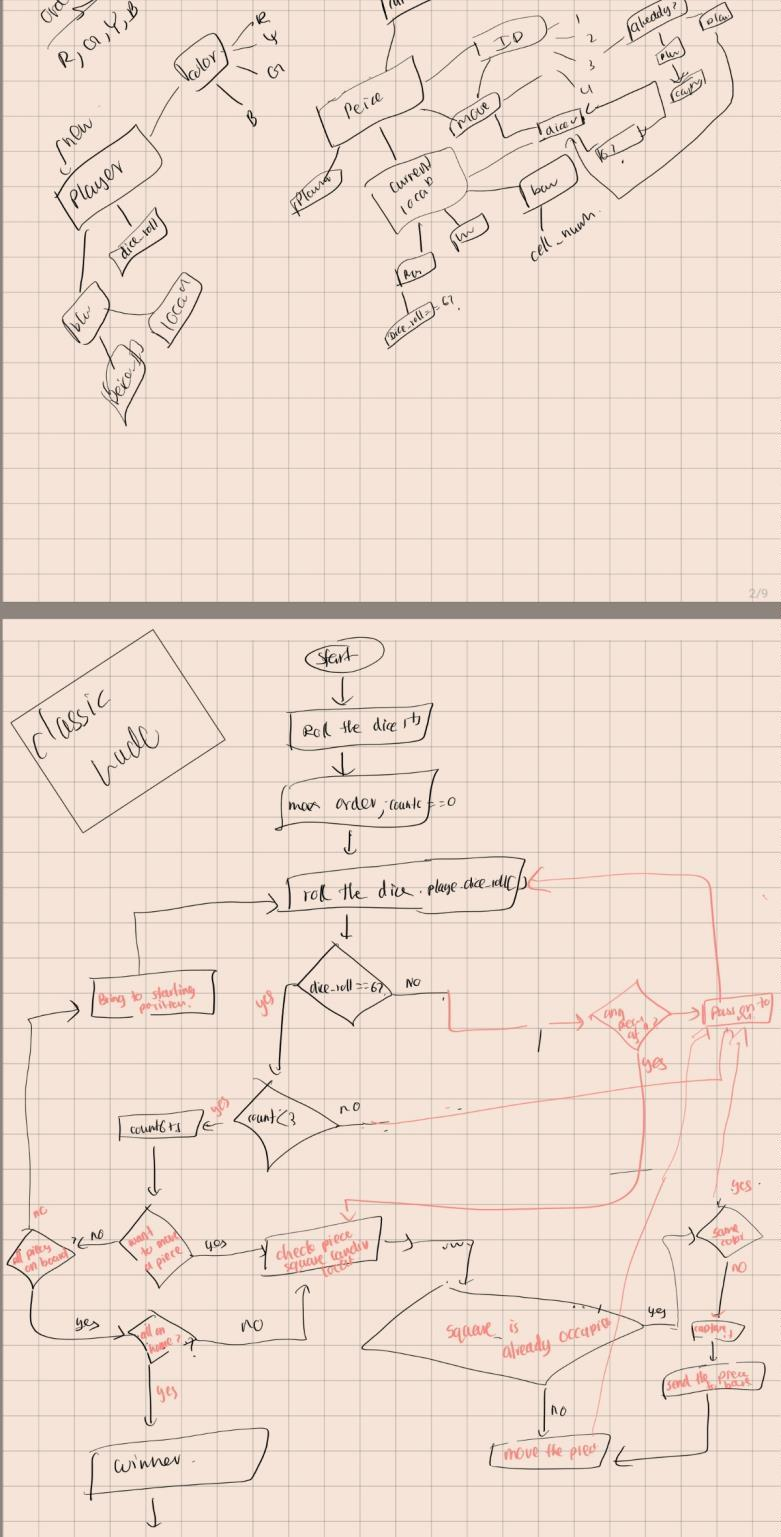
\includegraphics[width=281.4pt,height=553.6501pt]{latexImage_9029c54735fce5e87dc2f152105b4d6d.png}}
\end{picture}
\begin{tikzpicture}[overlay]
\path(0pt,0pt);
\filldraw[color_29791][even odd rule]
(9pt, -14.47998pt) -- (9.48pt, -14.47998pt)
 -- (9.48pt, -14.47998pt)
 -- (9.48pt, -14pt)
 -- (9.48pt, -14pt)
 -- (9pt, -14pt) -- cycle
;
\filldraw[color_29791][even odd rule]
(9pt, -14.47998pt) -- (9.48pt, -14.47998pt)
 -- (9.48pt, -14.47998pt)
 -- (9.48pt, -14pt)
 -- (9.48pt, -14pt)
 -- (9pt, -14pt) -- cycle
;
\filldraw[color_29791][even odd rule]
(9.48pt, -14.47998pt) -- (572.64pt, -14.47998pt)
 -- (572.64pt, -14.47998pt)
 -- (572.64pt, -14pt)
 -- (572.64pt, -14pt)
 -- (9.48pt, -14pt) -- cycle
;
\filldraw[color_29791][even odd rule]
(572.64pt, -14.47998pt) -- (573.12pt, -14.47998pt)
 -- (573.12pt, -14.47998pt)
 -- (573.12pt, -14pt)
 -- (573.12pt, -14pt)
 -- (572.64pt, -14pt) -- cycle
;
\filldraw[color_29791][even odd rule]
(572.64pt, -14.47998pt) -- (573.12pt, -14.47998pt)
 -- (573.12pt, -14.47998pt)
 -- (573.12pt, -14pt)
 -- (573.12pt, -14pt)
 -- (572.64pt, -14pt) -- cycle
;
\filldraw[color_29791][even odd rule]
(9pt, -757.64pt) -- (9.48pt, -757.64pt)
 -- (9.48pt, -757.64pt)
 -- (9.48pt, -14.48004pt)
 -- (9.48pt, -14.48004pt)
 -- (9pt, -14.48004pt) -- cycle
;
\filldraw[color_29791][even odd rule]
(572.64pt, -757.64pt) -- (573.12pt, -757.64pt)
 -- (573.12pt, -757.64pt)
 -- (573.12pt, -14.48004pt)
 -- (573.12pt, -14.48004pt)
 -- (572.64pt, -14.48004pt) -- cycle
;
\filldraw[color_29791][even odd rule]
(9pt, -758.12pt) -- (9.48pt, -758.12pt)
 -- (9.48pt, -758.12pt)
 -- (9.48pt, -757.64pt)
 -- (9.48pt, -757.64pt)
 -- (9pt, -757.64pt) -- cycle
;
\filldraw[color_29791][even odd rule]
(9pt, -758.12pt) -- (9.48pt, -758.12pt)
 -- (9.48pt, -758.12pt)
 -- (9.48pt, -757.64pt)
 -- (9.48pt, -757.64pt)
 -- (9pt, -757.64pt) -- cycle
;
\filldraw[color_29791][even odd rule]
(9.48pt, -758.12pt) -- (572.64pt, -758.12pt)
 -- (572.64pt, -758.12pt)
 -- (572.64pt, -757.64pt)
 -- (572.64pt, -757.64pt)
 -- (9.48pt, -757.64pt) -- cycle
;
\filldraw[color_29791][even odd rule]
(572.64pt, -758.12pt) -- (573.12pt, -758.12pt)
 -- (573.12pt, -758.12pt)
 -- (573.12pt, -757.64pt)
 -- (573.12pt, -757.64pt)
 -- (572.64pt, -757.64pt) -- cycle
;
\end{tikzpicture}
\newpage
\begin{tikzpicture}[overlay]
\path(0pt,0pt);
\filldraw[color_29791][even odd rule]
(572.64pt, -758.12pt) -- (573.12pt, -758.12pt)
 -- (573.12pt, -758.12pt)
 -- (573.12pt, -757.64pt)
 -- (573.12pt, -757.64pt)
 -- (572.64pt, -757.64pt) -- cycle
;
\begin{scope}
\clip
(57pt, -534.5pt) -- (445.8pt, -534.5pt)
 -- (445.8pt, -534.5pt)
 -- (445.8pt, -62pt)
 -- (445.8pt, -62pt)
 -- (57pt, -62pt) -- cycle
;
\end{scope}
\end{tikzpicture}
\begin{picture}(-5,0)(2.5,0)
\put(57,-534.5){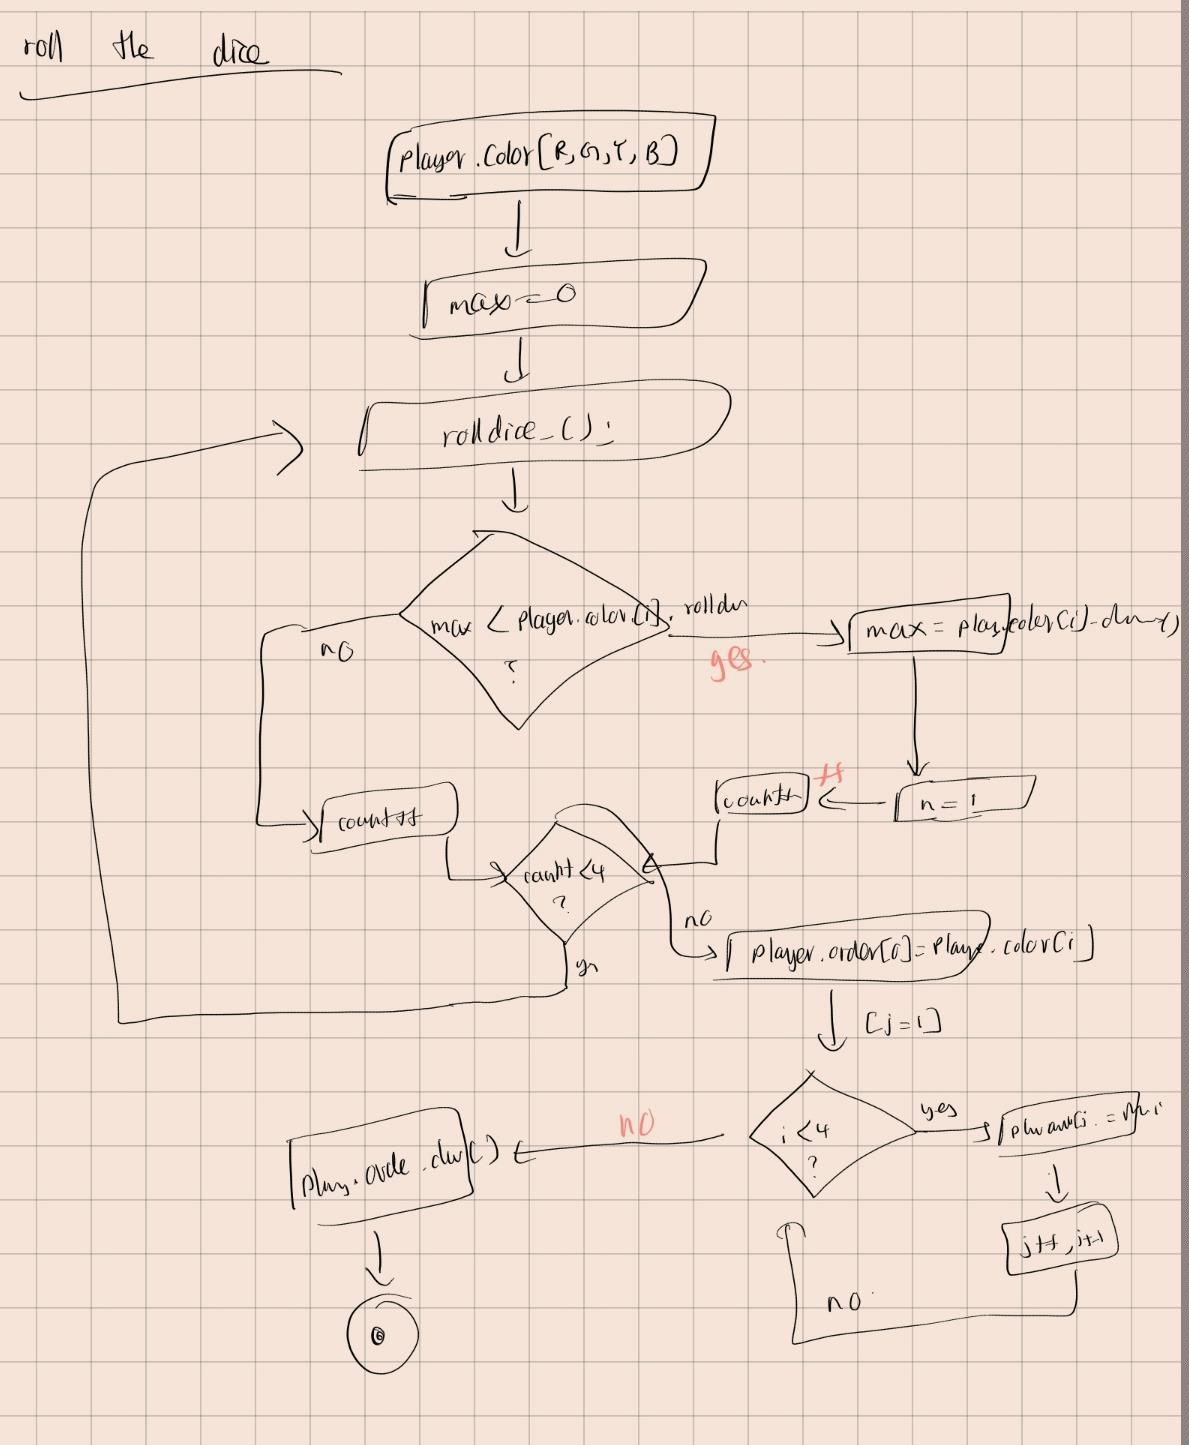
\includegraphics[width=388.8pt,height=472.5pt]{latexImage_b6e8e33860adec8c11f436acbe184ec8.png}}
\end{picture}
\begin{tikzpicture}[overlay]
\path(0pt,0pt);
\filldraw[color_29791][even odd rule]
(9pt, -14.47998pt) -- (9.48pt, -14.47998pt)
 -- (9.48pt, -14.47998pt)
 -- (9.48pt, -14pt)
 -- (9.48pt, -14pt)
 -- (9pt, -14pt) -- cycle
;
\filldraw[color_29791][even odd rule]
(9pt, -14.47998pt) -- (9.48pt, -14.47998pt)
 -- (9.48pt, -14.47998pt)
 -- (9.48pt, -14pt)
 -- (9.48pt, -14pt)
 -- (9pt, -14pt) -- cycle
;
\filldraw[color_29791][even odd rule]
(9.48pt, -14.47998pt) -- (572.64pt, -14.47998pt)
 -- (572.64pt, -14.47998pt)
 -- (572.64pt, -14pt)
 -- (572.64pt, -14pt)
 -- (9.48pt, -14pt) -- cycle
;
\filldraw[color_29791][even odd rule]
(572.64pt, -14.47998pt) -- (573.12pt, -14.47998pt)
 -- (573.12pt, -14.47998pt)
 -- (573.12pt, -14pt)
 -- (573.12pt, -14pt)
 -- (572.64pt, -14pt) -- cycle
;
\filldraw[color_29791][even odd rule]
(572.64pt, -14.47998pt) -- (573.12pt, -14.47998pt)
 -- (573.12pt, -14.47998pt)
 -- (573.12pt, -14pt)
 -- (573.12pt, -14pt)
 -- (572.64pt, -14pt) -- cycle
;
\filldraw[color_29791][even odd rule]
(9pt, -757.64pt) -- (9.48pt, -757.64pt)
 -- (9.48pt, -757.64pt)
 -- (9.48pt, -14.48004pt)
 -- (9.48pt, -14.48004pt)
 -- (9pt, -14.48004pt) -- cycle
;
\filldraw[color_29791][even odd rule]
(572.64pt, -757.64pt) -- (573.12pt, -757.64pt)
 -- (573.12pt, -757.64pt)
 -- (573.12pt, -14.48004pt)
 -- (573.12pt, -14.48004pt)
 -- (572.64pt, -14.48004pt) -- cycle
;
\filldraw[color_29791][even odd rule]
(9pt, -758.12pt) -- (9.48pt, -758.12pt)
 -- (9.48pt, -758.12pt)
 -- (9.48pt, -757.64pt)
 -- (9.48pt, -757.64pt)
 -- (9pt, -757.64pt) -- cycle
;
\filldraw[color_29791][even odd rule]
(9pt, -758.12pt) -- (9.48pt, -758.12pt)
 -- (9.48pt, -758.12pt)
 -- (9.48pt, -757.64pt)
 -- (9.48pt, -757.64pt)
 -- (9pt, -757.64pt) -- cycle
;
\filldraw[color_29791][even odd rule]
(9.48pt, -758.12pt) -- (572.64pt, -758.12pt)
 -- (572.64pt, -758.12pt)
 -- (572.64pt, -757.64pt)
 -- (572.64pt, -757.64pt)
 -- (9.48pt, -757.64pt) -- cycle
;
\filldraw[color_29791][even odd rule]
(572.64pt, -758.12pt) -- (573.12pt, -758.12pt)
 -- (573.12pt, -758.12pt)
 -- (573.12pt, -757.64pt)
 -- (573.12pt, -757.64pt)
 -- (572.64pt, -757.64pt) -- cycle
;
\end{tikzpicture}
\newpage
\begin{tikzpicture}[overlay]
\path(0pt,0pt);
\filldraw[color_29791][even odd rule]
(572.64pt, -758.12pt) -- (573.12pt, -758.12pt)
 -- (573.12pt, -758.12pt)
 -- (573.12pt, -757.64pt)
 -- (573.12pt, -757.64pt)
 -- (572.64pt, -757.64pt) -- cycle
;
\begin{scope}
\clip
(57pt, -379.65pt) -- (424.15pt, -379.65pt)
 -- (424.15pt, -379.65pt)
 -- (424.15pt, -62pt)
 -- (424.15pt, -62pt)
 -- (57pt, -62pt) -- cycle
;
\end{scope}
\end{tikzpicture}
\begin{picture}(-5,0)(2.5,0)
\put(57,-379.65){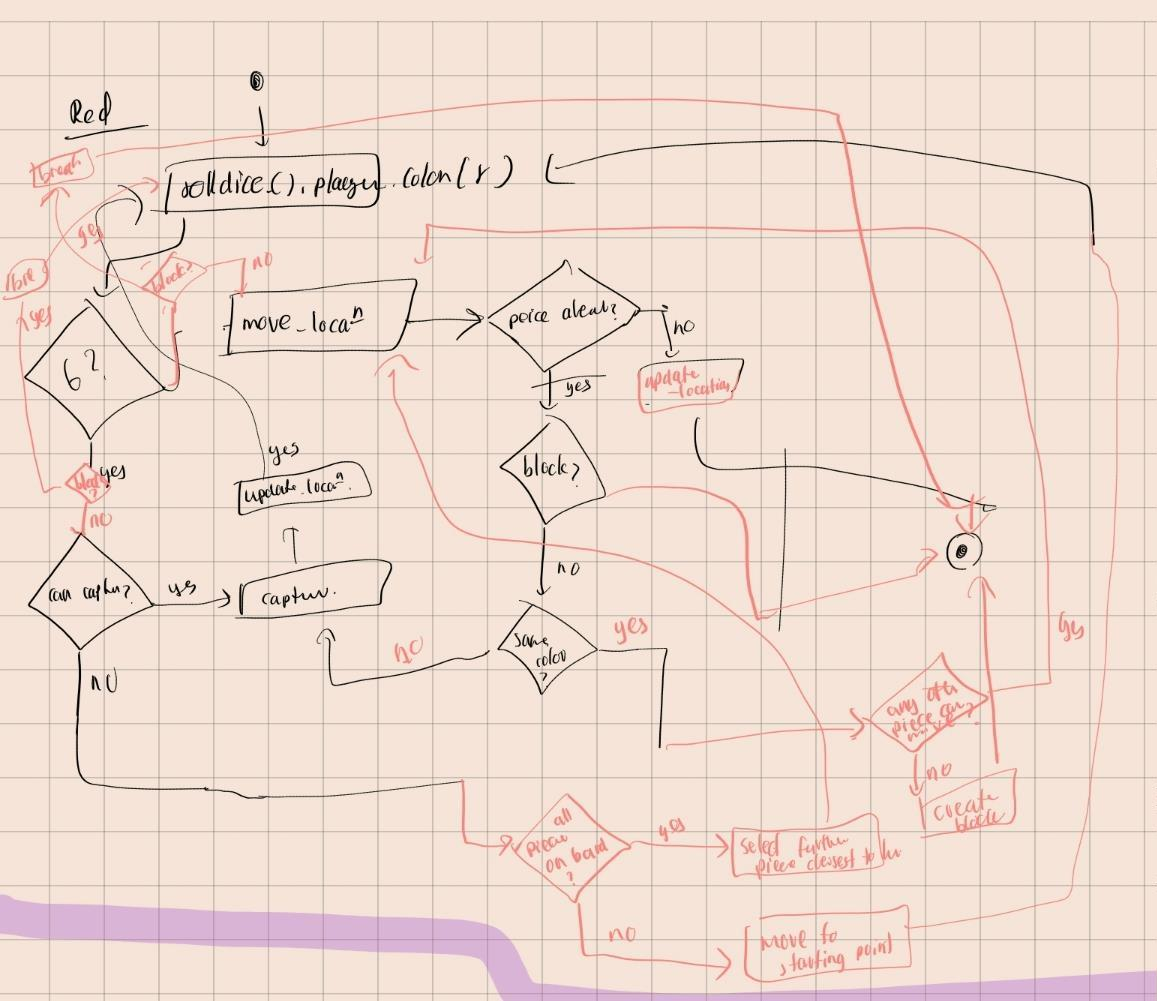
\includegraphics[width=367.15pt,height=317.65pt]{latexImage_8ca01c5c688601ed0c804a013643c432.png}}
\put(57,-685.9){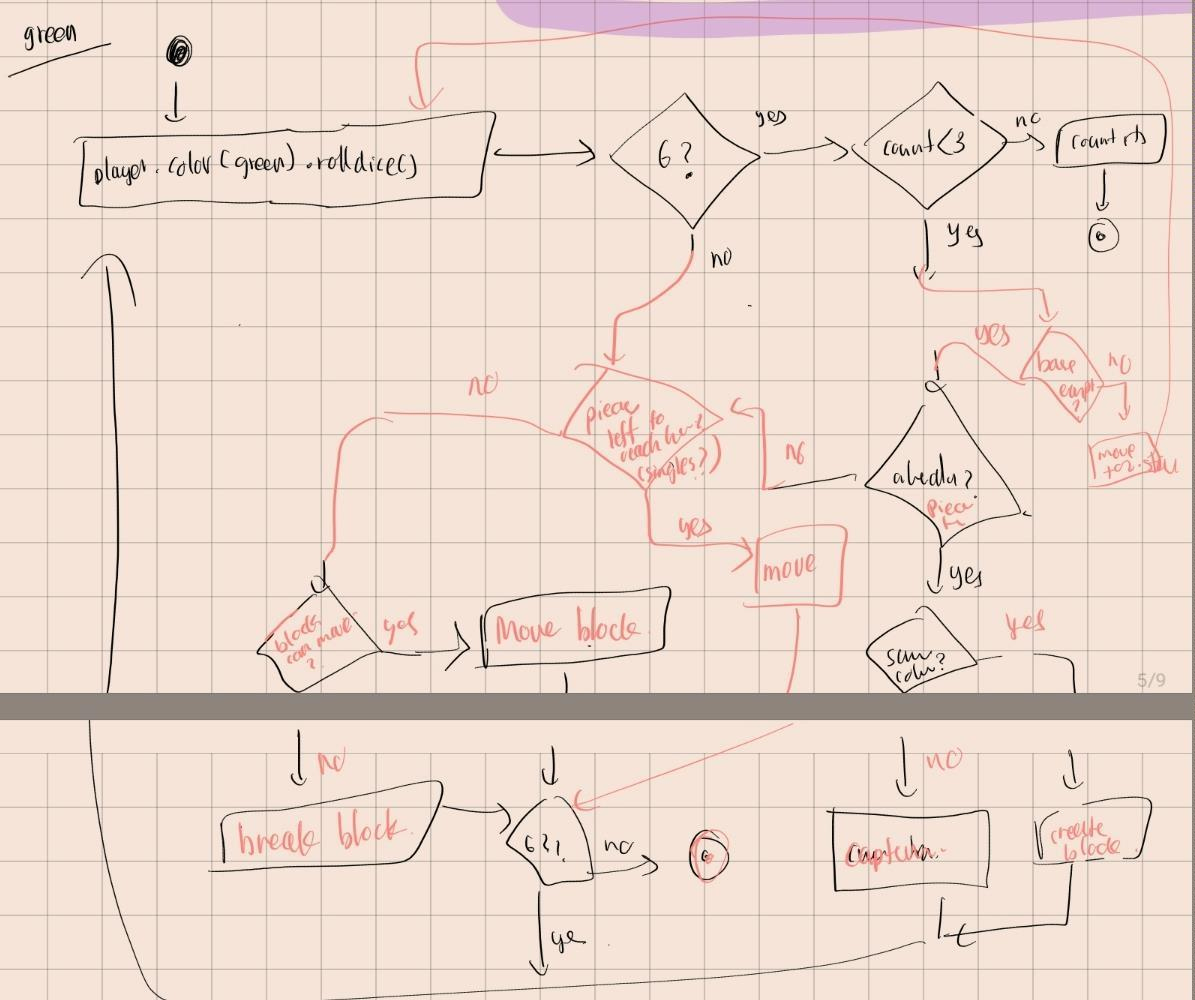
\includegraphics[width=365.95pt,height=306.25pt]{latexImage_69f00596dbee6cf7e6c11b7ef2c5fd16.png}}
\end{picture}
\begin{tikzpicture}[overlay]
\path(0pt,0pt);
\filldraw[color_29791][even odd rule]
(9pt, -14.47998pt) -- (9.48pt, -14.47998pt)
 -- (9.48pt, -14.47998pt)
 -- (9.48pt, -14pt)
 -- (9.48pt, -14pt)
 -- (9pt, -14pt) -- cycle
;
\filldraw[color_29791][even odd rule]
(9pt, -14.47998pt) -- (9.48pt, -14.47998pt)
 -- (9.48pt, -14.47998pt)
 -- (9.48pt, -14pt)
 -- (9.48pt, -14pt)
 -- (9pt, -14pt) -- cycle
;
\filldraw[color_29791][even odd rule]
(9.48pt, -14.47998pt) -- (572.64pt, -14.47998pt)
 -- (572.64pt, -14.47998pt)
 -- (572.64pt, -14pt)
 -- (572.64pt, -14pt)
 -- (9.48pt, -14pt) -- cycle
;
\filldraw[color_29791][even odd rule]
(572.64pt, -14.47998pt) -- (573.12pt, -14.47998pt)
 -- (573.12pt, -14.47998pt)
 -- (573.12pt, -14pt)
 -- (573.12pt, -14pt)
 -- (572.64pt, -14pt) -- cycle
;
\filldraw[color_29791][even odd rule]
(572.64pt, -14.47998pt) -- (573.12pt, -14.47998pt)
 -- (573.12pt, -14.47998pt)
 -- (573.12pt, -14pt)
 -- (573.12pt, -14pt)
 -- (572.64pt, -14pt) -- cycle
;
\filldraw[color_29791][even odd rule]
(9pt, -757.64pt) -- (9.48pt, -757.64pt)
 -- (9.48pt, -757.64pt)
 -- (9.48pt, -14.48004pt)
 -- (9.48pt, -14.48004pt)
 -- (9pt, -14.48004pt) -- cycle
;
\filldraw[color_29791][even odd rule]
(572.64pt, -757.64pt) -- (573.12pt, -757.64pt)
 -- (573.12pt, -757.64pt)
 -- (573.12pt, -14.48004pt)
 -- (573.12pt, -14.48004pt)
 -- (572.64pt, -14.48004pt) -- cycle
;
\filldraw[color_29791][even odd rule]
(9pt, -758.12pt) -- (9.48pt, -758.12pt)
 -- (9.48pt, -758.12pt)
 -- (9.48pt, -757.64pt)
 -- (9.48pt, -757.64pt)
 -- (9pt, -757.64pt) -- cycle
;
\filldraw[color_29791][even odd rule]
(9pt, -758.12pt) -- (9.48pt, -758.12pt)
 -- (9.48pt, -758.12pt)
 -- (9.48pt, -757.64pt)
 -- (9.48pt, -757.64pt)
 -- (9pt, -757.64pt) -- cycle
;
\filldraw[color_29791][even odd rule]
(9.48pt, -758.12pt) -- (572.64pt, -758.12pt)
 -- (572.64pt, -758.12pt)
 -- (572.64pt, -757.64pt)
 -- (572.64pt, -757.64pt)
 -- (9.48pt, -757.64pt) -- cycle
;
\filldraw[color_29791][even odd rule]
(572.64pt, -758.12pt) -- (573.12pt, -758.12pt)
 -- (573.12pt, -758.12pt)
 -- (573.12pt, -757.64pt)
 -- (573.12pt, -757.64pt)
 -- (572.64pt, -757.64pt) -- cycle
;
\end{tikzpicture}
\newpage
\begin{tikzpicture}[overlay]
\path(0pt,0pt);
\filldraw[color_29791][even odd rule]
(572.64pt, -758.12pt) -- (573.12pt, -758.12pt)
 -- (573.12pt, -758.12pt)
 -- (573.12pt, -757.64pt)
 -- (573.12pt, -757.64pt)
 -- (572.64pt, -757.64pt) -- cycle
;
\begin{scope}
\clip
(57pt, -608.6pt) -- (525pt, -608.6pt)
 -- (525pt, -608.6pt)
 -- (525pt, -62pt)
 -- (525pt, -62pt)
 -- (57pt, -62pt) -- cycle
;
\end{scope}
\end{tikzpicture}
\begin{picture}(-5,0)(2.5,0)
\put(57,-608.65){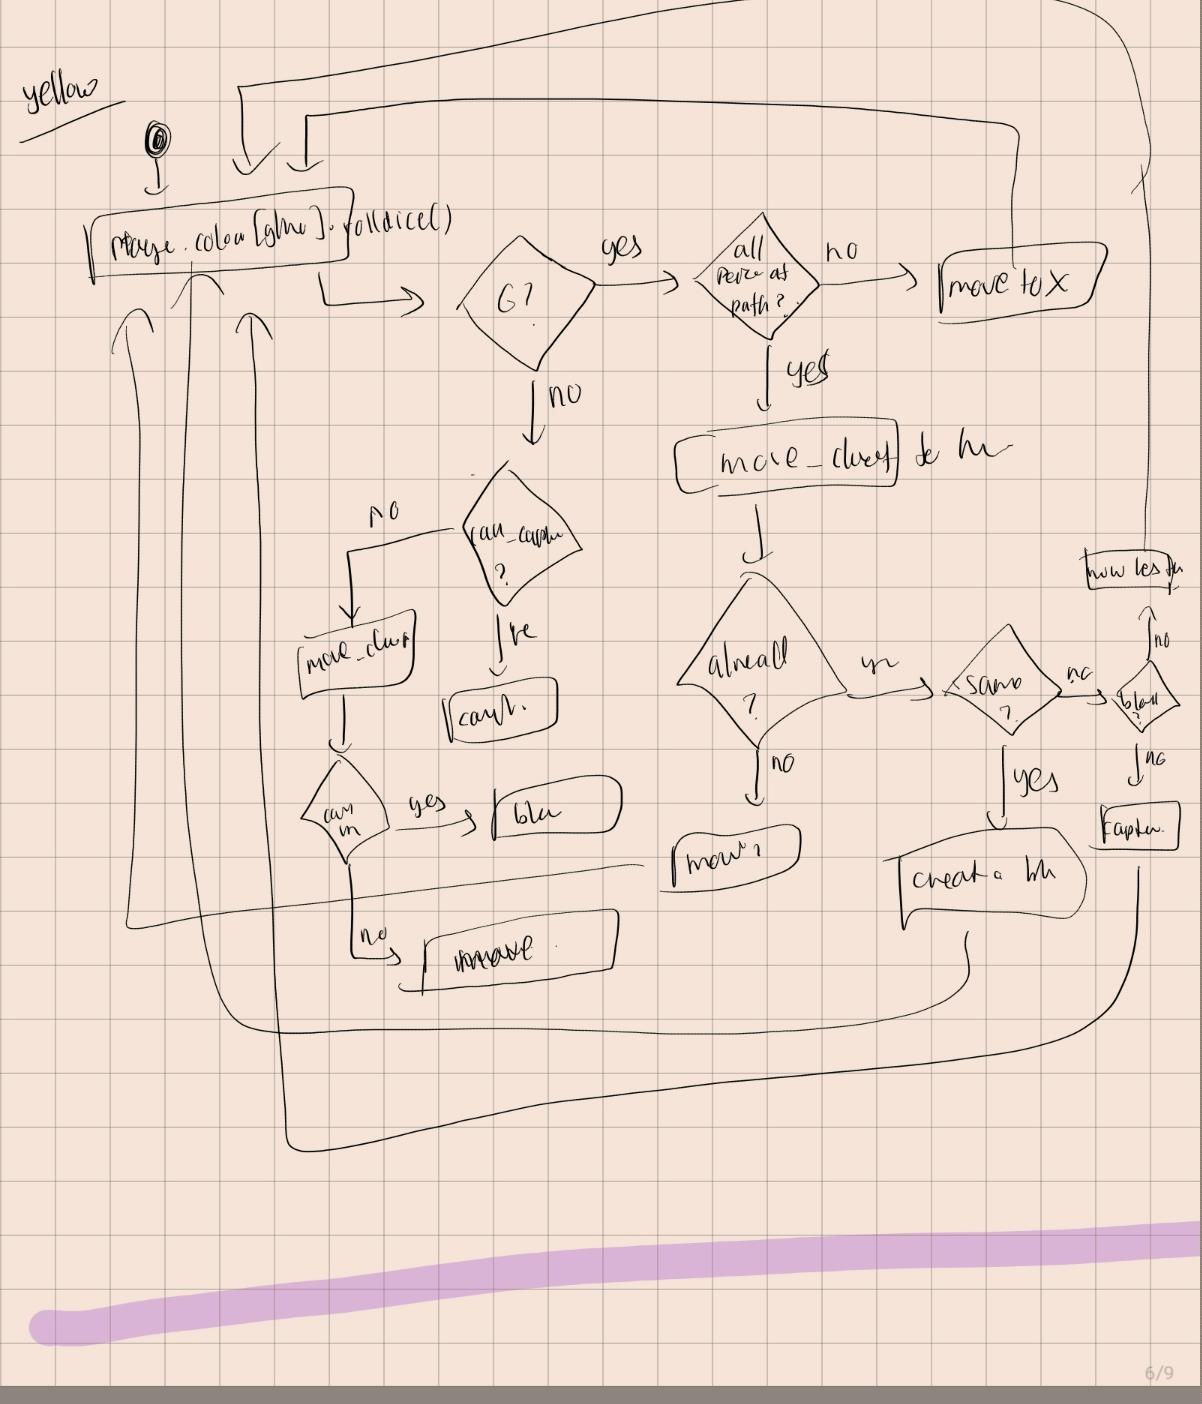
\includegraphics[width=468pt,height=546.65pt]{latexImage_c448ec5440c4cbd511ab0ba5599bd5e5.png}}
\end{picture}
\begin{tikzpicture}[overlay]
\path(0pt,0pt);
\filldraw[color_29791][even odd rule]
(9pt, -14.47998pt) -- (9.48pt, -14.47998pt)
 -- (9.48pt, -14.47998pt)
 -- (9.48pt, -14pt)
 -- (9.48pt, -14pt)
 -- (9pt, -14pt) -- cycle
;
\filldraw[color_29791][even odd rule]
(9pt, -14.47998pt) -- (9.48pt, -14.47998pt)
 -- (9.48pt, -14.47998pt)
 -- (9.48pt, -14pt)
 -- (9.48pt, -14pt)
 -- (9pt, -14pt) -- cycle
;
\filldraw[color_29791][even odd rule]
(9.48pt, -14.47998pt) -- (572.64pt, -14.47998pt)
 -- (572.64pt, -14.47998pt)
 -- (572.64pt, -14pt)
 -- (572.64pt, -14pt)
 -- (9.48pt, -14pt) -- cycle
;
\filldraw[color_29791][even odd rule]
(572.64pt, -14.47998pt) -- (573.12pt, -14.47998pt)
 -- (573.12pt, -14.47998pt)
 -- (573.12pt, -14pt)
 -- (573.12pt, -14pt)
 -- (572.64pt, -14pt) -- cycle
;
\filldraw[color_29791][even odd rule]
(572.64pt, -14.47998pt) -- (573.12pt, -14.47998pt)
 -- (573.12pt, -14.47998pt)
 -- (573.12pt, -14pt)
 -- (573.12pt, -14pt)
 -- (572.64pt, -14pt) -- cycle
;
\filldraw[color_29791][even odd rule]
(9pt, -757.64pt) -- (9.48pt, -757.64pt)
 -- (9.48pt, -757.64pt)
 -- (9.48pt, -14.48004pt)
 -- (9.48pt, -14.48004pt)
 -- (9pt, -14.48004pt) -- cycle
;
\filldraw[color_29791][even odd rule]
(572.64pt, -757.64pt) -- (573.12pt, -757.64pt)
 -- (573.12pt, -757.64pt)
 -- (573.12pt, -14.48004pt)
 -- (573.12pt, -14.48004pt)
 -- (572.64pt, -14.48004pt) -- cycle
;
\filldraw[color_29791][even odd rule]
(9pt, -758.12pt) -- (9.48pt, -758.12pt)
 -- (9.48pt, -758.12pt)
 -- (9.48pt, -757.64pt)
 -- (9.48pt, -757.64pt)
 -- (9pt, -757.64pt) -- cycle
;
\filldraw[color_29791][even odd rule]
(9pt, -758.12pt) -- (9.48pt, -758.12pt)
 -- (9.48pt, -758.12pt)
 -- (9.48pt, -757.64pt)
 -- (9.48pt, -757.64pt)
 -- (9pt, -757.64pt) -- cycle
;
\filldraw[color_29791][even odd rule]
(9.48pt, -758.12pt) -- (572.64pt, -758.12pt)
 -- (572.64pt, -758.12pt)
 -- (572.64pt, -757.64pt)
 -- (572.64pt, -757.64pt)
 -- (9.48pt, -757.64pt) -- cycle
;
\filldraw[color_29791][even odd rule]
(572.64pt, -758.12pt) -- (573.12pt, -758.12pt)
 -- (573.12pt, -758.12pt)
 -- (573.12pt, -757.64pt)
 -- (573.12pt, -757.64pt)
 -- (572.64pt, -757.64pt) -- cycle
;
\filldraw[color_29791][even odd rule]
(572.64pt, -758.12pt) -- (573.12pt, -758.12pt)
 -- (573.12pt, -758.12pt)
 -- (573.12pt, -757.64pt)
 -- (573.12pt, -757.64pt)
 -- (572.64pt, -757.64pt) -- cycle
;
\end{tikzpicture}
\newpage
\begin{tikzpicture}[overlay]\path(0pt,0pt);\end{tikzpicture}
\begin{picture}(-5,0)(2.5,0)
\put(525.1,-400.45){\fontsize{11.04}{1}\usefont{T1}{cmr}{m}{n}\selectfont\color{color_29791} }
\put(57,-400.4){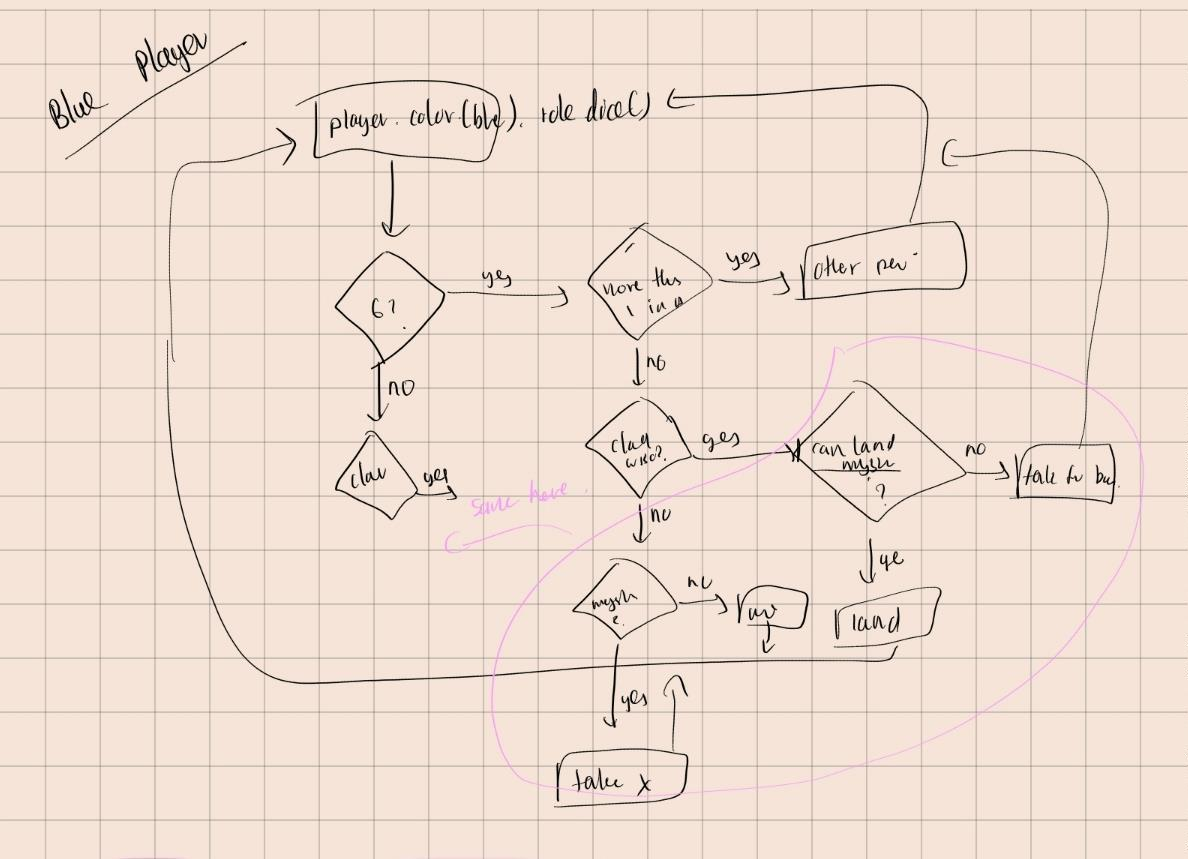
\includegraphics[width=468pt,height=338.4pt]{latexImage_490584c2458a4a6ce4234ef1478dc07d.png}}
\put(75.024,-437.43){\fontsize{11.04}{1}\usefont{T1}{cmr}{m}{n}\selectfont\color{color_29791}reference used for latex template : - openleaf.com}

\end{picture}
\begin{tikzpicture}[overlay]
\path(0pt,0pt);
\filldraw[color_29791][even odd rule]
(9pt, -14.47998pt) -- (9.48pt, -14.47998pt)
 -- (9.48pt, -14.47998pt)
 -- (9.48pt, -14pt)
 -- (9.48pt, -14pt)
 -- (9pt, -14pt) -- cycle
;
\filldraw[color_29791][even odd rule]
(9pt, -14.47998pt) -- (9.48pt, -14.47998pt)
 -- (9.48pt, -14.47998pt)
 -- (9.48pt, -14pt)
 -- (9.48pt, -14pt)
 -- (9pt, -14pt) -- cycle
;
\filldraw[color_29791][even odd rule]
(9.48pt, -14.47998pt) -- (572.64pt, -14.47998pt)
 -- (572.64pt, -14.47998pt)
 -- (572.64pt, -14pt)
 -- (572.64pt, -14pt)
 -- (9.48pt, -14pt) -- cycle
;
\filldraw[color_29791][even odd rule]
(572.64pt, -14.47998pt) -- (573.12pt, -14.47998pt)
 -- (573.12pt, -14.47998pt)
 -- (573.12pt, -14pt)
 -- (573.12pt, -14pt)
 -- (572.64pt, -14pt) -- cycle
;
\filldraw[color_29791][even odd rule]
(572.64pt, -14.47998pt) -- (573.12pt, -14.47998pt)
 -- (573.12pt, -14.47998pt)
 -- (573.12pt, -14pt)
 -- (573.12pt, -14pt)
 -- (572.64pt, -14pt) -- cycle
;
\filldraw[color_29791][even odd rule]
(9pt, -757.64pt) -- (9.48pt, -757.64pt)
 -- (9.48pt, -757.64pt)
 -- (9.48pt, -14.48004pt)
 -- (9.48pt, -14.48004pt)
 -- (9pt, -14.48004pt) -- cycle
;
\filldraw[color_29791][even odd rule]
(572.64pt, -757.64pt) -- (573.12pt, -757.64pt)
 -- (573.12pt, -757.64pt)
 -- (573.12pt, -14.48004pt)
 -- (573.12pt, -14.48004pt)
 -- (572.64pt, -14.48004pt) -- cycle
;
\filldraw[color_29791][even odd rule]
(9pt, -758.12pt) -- (9.48pt, -758.12pt)
 -- (9.48pt, -758.12pt)
 -- (9.48pt, -757.64pt)
 -- (9.48pt, -757.64pt)
 -- (9pt, -757.64pt) -- cycle
;
\filldraw[color_29791][even odd rule]
(9pt, -758.12pt) -- (9.48pt, -758.12pt)
 -- (9.48pt, -758.12pt)
 -- (9.48pt, -757.64pt)
 -- (9.48pt, -757.64pt)
 -- (9pt, -757.64pt) -- cycle
;
\filldraw[color_29791][even odd rule]
(9.48pt, -758.12pt) -- (572.64pt, -758.12pt)
 -- (572.64pt, -758.12pt)
 -- (572.64pt, -757.64pt)
 -- (572.64pt, -757.64pt)
 -- (9.48pt, -757.64pt) -- cycle
;
\filldraw[color_29791][even odd rule]
(572.64pt, -758.12pt) -- (573.12pt, -758.12pt)
 -- (573.12pt, -758.12pt)
 -- (573.12pt, -757.64pt)
 -- (573.12pt, -757.64pt)
 -- (572.64pt, -757.64pt) -- cycle
;
\filldraw[color_29791][even odd rule]
(572.64pt, -758.12pt) -- (573.12pt, -758.12pt)
 -- (573.12pt, -758.12pt)
 -- (573.12pt, -757.64pt)
 -- (573.12pt, -757.64pt)
 -- (572.64pt, -757.64pt) -- cycle
;
\end{tikzpicture}


\end{document}